% Esta plantilla ha sido diseñada por Daniel del Río Velilla, profesor en la Escuela de Aeronáutica y del Espacio, UPM.
% LA PLANTILLA ES DE USO LIBRE PERO ESTÁ SUJETA A DERECHOS DE PROPIEDAD INTELECTUAL, POR LO QUE SU COMERCIALIZACIÓN ES ILEGAL.

\documentclass[11pt,a4paper,titlepage,twoside]{report}

%   ---   DEFINICION DEL TRABAJO   ---   %

\newcommand{\Project}{Trabajo de Fin de Grado}
\newcommand{\ProjectTitle}{Desarrollo de una herramienta en Python para el postprocesado y comparación de múltiples casos transitorios pertenecientes a un modelo térmico diseñado en ESATAN-TMS}
\newcommand{\ProjectSubject}{ESPECIALIDAD: Propulsión Aeroespacial}
\newcommand{\ProjectAutor}{ Asier Fiel Mariblanca}
\newcommand{\ProjectTutor}{ David González Bárcena}
\newcommand{\ProjectLocation}{Madrid}
\newcommand{\ProjectDate}{septiembre 2026}

% Descomentar si se tiene un repositorio del trabajo
\newcommand{\ProjectGitHub}{https://github.com/asi1803/TFG/tree/main/TFG_Asier}



%   ---   INCLUIR ARCHIVOS DE CONFIGURACION   ---   %

\input{./Tex_Files/packages.tex}
\input{./Tex_Files/header_footer.tex}
\makeatletter

\newcommand{\clearemptydoublepage}{%
    \clearpage
    \if@twoside
        \ifodd\value{page}
            % The next page is already odd: no blank page is required.
        \else
            % Insert an empty even page so that the next page is odd.
            \thispagestyle{empty}%
            \null
            \newpage
        \fi
    \fi
}

\makeatother


\newcommand{\blankpage}{%
    \null
    \thispagestyle{empty}%
    \newpage
}
%FORMA DE QUE APAREZCAN LOS ACRÓNIMOS
% ACRONIMOS A INCLUIR
\newacronym{esa}{ESA}{European Space Agency}
%\acrshort{esa},\acrlong{esa}
\newacronym{esatan-tms}{ESATAN-TMS}{European Space Agency Thermal Analysis Tool}
\newacronym{tcs}{TCS}{Thermal Control System}
\newacronym{lpm}{LPM}{Lumped Parameter Method}
\newacronym{etsiae}{ETSIAE}{Escuela Técnica Superior de Ingeniería Aeronáutica y del Espacio}
\newacronym{idr}{IDR}{Instituto Universitario de Microgravedad "Ignacio Da Riva"}
\newacronym{fdm}{FDM}{Finite-Difference Method}
\newacronym{fem}{FEM}{Finite-Element Method}
\newacronym{fvm}{FVM}{Finite-Volume Method}
\newacronym{mli}{MLI}{Multi-Layer Insulation}
\newacronym{obc}{OBC}{On-Board Computer}
\newacronym{adcs}{ADCS}{Attitude Determination and Control System}
\newacronym{osr}{OSR}{Optical Solar Reflector}
\newacronym{ito}{ITO}{Indium Tin Oxide}
\newacronym{nasa}{NASA}{National Aeronautics and Space Administration}
\newacronym{thermica}{THERMICA}{THERMICA Suite} 
\newacronym{td}{TD}{Thermal Desktop} 
\newacronym{sinda-fluint}{SINDA/FLUINT}{Systems Improved Numerical Differencing Analyzer/Fluid Integrator} 
\newacronym{sst}{SST}{Simcenter 3D Space Systems Thermal} 
\newacronym{tasverter}{TASverter}{Thermal Analysis for Space converter} 
%Imprime los acrónimos sin titulo adicional
%\label{ch:acronyms}
%\printglossaries
%\printacronyms


% --- CREAR ESTILO PERSONALIZADO PARA ACRÓNIMOS ---
\newglossarystyle{estiloTFG}{
  \setglossarystyle{list} % Nos basamos en la lista base
  \renewcommand*{\glossentry}[2]{
    % ##1 es el acrónimo, ##2 es el número de página
    \item[] \noindent \glstarget{##1}{\glossentrydesc{##1} (\glossentryname{##1})} \dotfill ##2
  }
}

%   ---   AJUSTES PREVIOS  ---   %

\addto\captionsspanish{%
  \renewcommand{\bibname}{References}%
}
\addto\captionsspanish{%
  \renewcommand{\contentsname}{Contents} % O el nombre que prefieras
}

% Cambiar nombres de figuras, tablas y ecuaciones a inglés

% English names used throughout the document
\addto\captionsspanish{%
    \renewcommand{\chaptername}{Chapter}%
    \renewcommand{\figurename}{Figure}%
    \renewcommand{\tablename}{Table}%
}

% English names generated by \autoref
\addto\extrasspanish{%
    \renewcommand{\chapterautorefname}{Chapter}%
    \renewcommand{\sectionautorefname}{Section}%
    \renewcommand{\subsectionautorefname}{Section}%
    \renewcommand{\subsubsectionautorefname}{Section}%
    \renewcommand{\figureautorefname}{Figure}%
    \renewcommand{\tableautorefname}{Table}%
    \renewcommand{\equationautorefname}{Equation}%
}

%\addto\captionsspanish{%
%  \renewcommand{\figurename}{Figure}%
%  \renewcommand{\tablename}{Table}%
%}
% Para \autoref (hyperref)
%\addto\extrasenglish{%
%  \renewcommand{\figureautorefname}{Figure}%
%  \renewcommand{\tableautorefname}{Table}%
%  \renewcommand{\equationautorefname}{Equation}%
%}

%\addto\extrasspanish{%
%  \renewcommand{\figureautorefname}{Figure}%
%  \renewcommand{\tableautorefname}{Table}%
%  \renewcommand{\equationautorefname}{Equation}%
%}


% Formato de los capítulos: Número y título en la misma línea
\titleformat{\chapter}[hang]
  {\normalfont\huge\bfseries} % Estilo de la fuente
  {\thechapter.} % El número del capítulo seguido de un punto
  {1em} % Espacio horizontal entre el número y el título
  {} % Código antes del título

% Quitar el espacio gigante encima del título del capítulo
\titlespacing*{\chapter}{0pt}{-20pt}{30pt}

%   ---   COMIENZO DEL DOCUMENTO   ---   %

\begin{document}


%   ---   INCLUIR PORTADA   ---   %

\input{./Tex_Files/portada.tex}



%   ---   INDICE Y LISTAS   ---   %

% Indice
\pagenumbering{gobble}
\tableofcontents
\newpage

% Numeracion en romano
\pagenumbering{roman}
\raggedbottom

% Figuras   
\renewcommand{\listfigurename}{List of Figures} 
%\addcontentsline{toc}{section}{\listfigurename}
\listoffigures
\cleardoublepage

% Tablas
\renewcommand{\listtablename}{List of Tables}
%\addcontentsline{toc}{section}{\listtablename}
\listoftables
\cleardoublepage

% Acronyms 
%\chapter*{Acronyms}
%\addcontentsline{toc}{chapter}{Acronyms}
\setglossarystyle{estiloTFG}
\printglossary[type=\acronymtype, title=Acronyms]
\cleardoublepage

% Numeracion en arabico
\setcounter{page}{0}
\pagenumbering{arabic}



%   ---   ARCHIVOS DEL DOCUMENTO   ---   %
% Es recomendable escribir el trabajo en documentos separados y luego importarlos al main.
\chapter{Abstract} \label{ch:chapter_01}

This Bachelor's Thesis focuses on the development of a Python-based post-processing tool for the thermal 
analysis of space systems using results generated with \acrshort{esatan-tms}.

Building upon a previous study limited to the post-processing of steady-state radiative cases, 
this work extends the analysis to fully transient thermal simulations. In addition, the tool has been 
designed to handle and compare multiple simulation cases associated with the same thermal model, allowing a more 
complete assessment of the system response under different operating conditions and orbital scenarios.

Since \acrshort{esatan-tms} presents limitations regarding integrated data visualization and case-to-case 
comparison, this project implements custom post-processing routines in Python, using libraries such as 
NumPy, Pandas, and Matplotlib. These routines automate the extraction, organization, and visualization of 
nodal results, including temperature evolution curves, transient heat flows, and comparative plots between 
different cases.

The resulting methodology improves the interpretation of complex transient thermal results and provides a 
more flexible framework for evaluating the thermal performance of a system throughout realistic orbital 
thermal cycles. By enabling the simultaneous analysis of several cases belonging to the same 
model, the developed tool supports a more efficient and systematic validation of thermal behaviour 
in space applications.


\cleardoublepage

\chapter{Introduction}
\label{ch:introduction}

Thermal management is an essential part of spacecraft design, as the temperature
of each component must remain within allowable limits throughout the
mission. 

Since both the space environment and the operating conditions of the
spacecraft evolve across different mission phases, steady-state cases cannot fully represent the actual thermal response. 
Transient simulations are therefore needed to examine the evolution of temperatures and heat flows.

The design of a spacecraft thermal control system relies on numerical analysis
tools to predict system behaviour under different mission and operating
conditions. These tools are used to represent the spacecraft through a thermal
model and to calculate variables such as nodal temperatures and heat flows.
Some of the best-known tools include \acrshort{thermica}, \acrlong{td} together with \acrshort{sinda-fluint}, 
\acrfull{sst} and \acrshort{esatan-tms}, which provides a specialised 
environment for the development and solution of spacecraft thermal models.

The amount of information generated by these simulations can become
considerable, particularly when transient analyses or multiple cases of the
same model are considered. In such situations, the results must be organised
and represented in a way that allows their evolution to be examined and the
effects of the differences between cases to be identified. Dedicated
post-processing tools can therefore support the interpretation of the
simulation results.

This Bachelor’s Thesis builds on an existing Python-based post-processing tool
initially intended for steady-state analysis. The work combines the adaptation
of the tool to transient and multi-case analysis with the development of a
representative spacecraft thermal model in \acrshort{esatan-tms}. Selected
thermal results are also used to perform a simplified electrical power
analysis and provide the inputs for a separate battery model. The specific
objectives of the project are presented in the following section.

\section{Objectives}
\label{sec:objectives}

The main objective of the project is to enable the existing application to
process, analyse, and compare several transient cases associated with the same
\acrshort{esatan-tms} thermal model within a common environment.

Reaching this objective requires the coordinated development of the thermal
model and the post-processing tool. The \acrshort{esatan-tms} model provides
a consistent set of transient results, while the application is adapted to
manage and compare them. 

The thermal results are also used to estimate the electrical power generated
by the solar panels and to calculate the electrical power balance. These
calculations provide the inputs for a separate simplified battery model. 

Accordingly, the specific objectives of the project are:

\begin{itemize}
    \item Develop a representative spacecraft thermal model and define
    transient cases under different environmental and operating conditions.

    \item Adapt the existing application to load and manage several transient
    result files while retaining a common model hierarchy.

    \item Implement methods for representing and comparing temperatures,
    thermal loads, heat flows and exchanged thermal energy.

    \item Generate graphical outputs and summary tables, and allow the
    corresponding analyses and configurations to be saved, restored and
    exported.

    \item Estimate solar-panel electrical generation, calculate the electrical
    power balance and use the resulting power profiles as inputs to a separate
    simplified battery model.

    \item Apply the complete analysis process to the selected transient cases and compare
    the thermal responses obtained under different environmental and operating
    conditions.
\end{itemize}
\cleardoublepage

\chapter{State of the Art} 
\label{ch:state_of_the_art} 

Spacecraft thermal analyses are commonly performed using specialised software 
tools, including \acrshort{thermica}, \acrfull{td} coupled with 
\acrshort{sinda-fluint}, \acrshort{sst} and \acrshort{esatan-tms}
\cite{soriano2007thermica,wang2020shiiver,zarei2020simcenter}.
The result files generated by \acrshort{esatan-tms} contain a considerable amount of data 
that must be organised, examined, and interpreted to evaluate the thermal 
behaviour of the model. Two thermal regimes are considered in the
analysis. A steady-state analysis provides a time-independent thermal solution
for a predefined set of boundary conditions, whereas a transient analysis
describes the evolution of the calculated results throughout the simulated
period \cite{thermal_eng_man,esatan_user_man}.

An interactive Python-based post-processing tool facilitates the
interpretation of these results by extracting and organising the data generated
by \acrshort{esatan-tms} and presenting them through numerical and graphical
representations \cite{tfg_carol}. The initial implementation was tested
primarily with steady-state results from HELIOS, a thermal model developed in
\acrshort{esatan-tms}, and therefore focuses on a single steady-state case. The
extended application processes transient results and compares several cases
associated with the same thermal model.


\section{Post-Processing Capabilities in ESATAN-TMS} 
\label{sec:esatan_postprocessing} 

\acrshort{esatan-tms} supports the numerical solution of spacecraft thermal
models under both steady-state and transient conditions. For each analysis
case, the resulting dataset contains nodal temperatures, applied thermal loads, 
and conductive and radiative heat flows. The software provides numerical and 
graphical tools for examining these results 
\cite{esatan_user_man,esatan_training_man}.

The structure of the exported information depends on the selected outputs and
the type of analysis. Transient results associate each variable with successive
output times, and heat-flow data identify the nodes or surfaces involved in each
exchange. In every case, numerical identifiers must remain linked to the physical
elements they represent
\cite{esatan_user_man,esatan_training_man}.

These datasets provide the information required to evaluate the thermal
behaviour of the model. When transient analyses or several simulation cases
are considered, however, direct inspection can become less practical.
Relevant results must therefore be selected, organised, and compared
consistently.

The post-processing functions available in \acrshort{esatan-tms} may not cover
every requirement of a particular analysis. The Python implementation
complements these functions by reorganising the exported thermal data
according to an engineering hierarchy and providing additional methods for
selecting, grouping, and representing the results 
\cite{esatan_user_man}.

\section{Steady-State Thermal Model: HELIOS}  
\label{sec:helios_model}  

HELIOS is a thermal model developed in \acrshort{esatan-tms} with a single 
steady-state analysis case. The model supports the development and testing of the initial
Python-based tool. 
As a first approximation of a spacecraft thermal system, it
provides sufficient detail to generate a consistent set of thermal results.
The model contains the spacecraft structure, solar panels, batteries,
radiating surfaces, and multi-layer insulation. The different components are
connected through the conductive and radiative couplings that define the
thermal network of the model \cite{tfg_carol}.

The complete spacecraft configuration and a view of the internal components
are shown in Figure~\ref{fig:helios_geometry}.

\begin{figure}[H]
    \centering

    \begin{subfigure}[t]{0.8\textwidth}
        \centering
        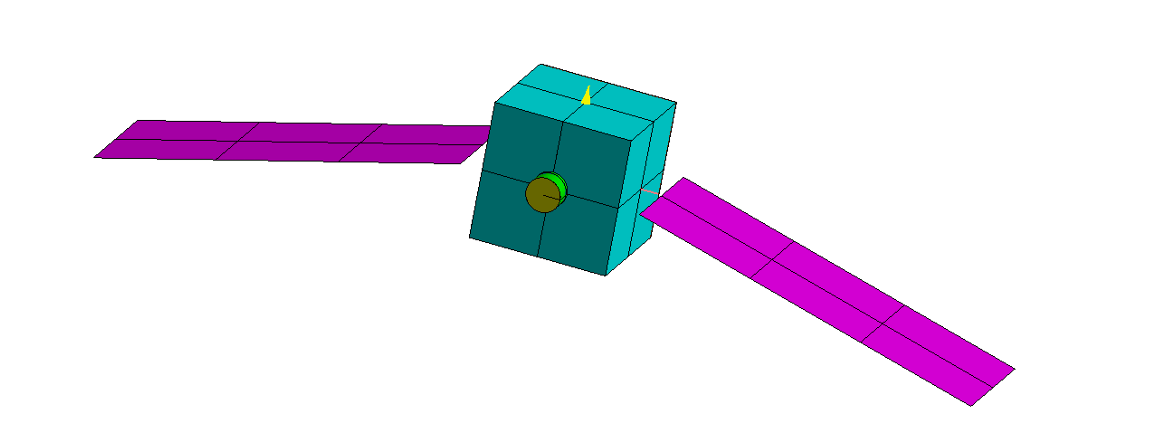
\includegraphics[width=\textwidth]{Figures/03/HELIOS.png}
        \caption{External view of the satellite model.}
        \label{fig:helios_external}
    \end{subfigure}

    \vspace{0.4cm}

    \begin{subfigure}[t]{0.9\textwidth}
        \centering
        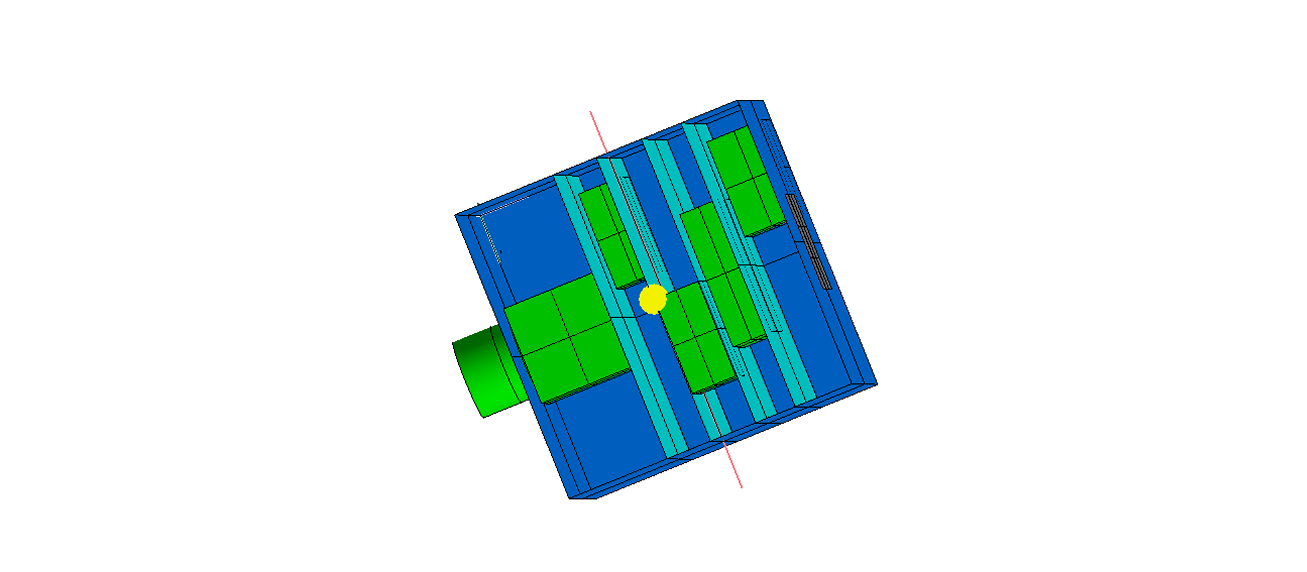
\includegraphics[width=\textwidth]{Figures/03/geom_HELIOS.png}
        \caption{Internal view of the satellite model.}
        \label{fig:helios_internal}
    \end{subfigure}

    \caption{External and internal views of the HELIOS thermal model. Taken
    from \cite{tfg_carol}.}
    \label{fig:helios_geometry}
\end{figure}

The steady-state solution of HELIOS contains the thermal data that are
extracted and organised by the initial Python code before being examined
through the graphical interface. The application developed for this thesis uses
a separate spacecraft thermal model with several cyclic transient analysis
cases.

\section{Python-Based Post-Processing of Steady-State Cases} 
\label{sec:previous_application} 

The initial Python-based implementation uses the steady-state results generated
for the HELIOS model in \acrshort{esatan-tms}~\cite{tfg_carol}. In this type
of analysis, a single temperature is calculated for each node under the
selected boundary conditions, while the corresponding thermal loads and heat
flows remain independent of time.

The imported results are linked to the hierarchy defined for the thermal
model, so that each node can be located within the corresponding component and
subsystem. Instead of working directly with the complete list of node
identifiers contained in the \acrshort{esatan-tms} files, the user can examine
the results through the spacecraft structure. This relationship between the
thermal data and the physical model helps identify the origin of each value and
interpret it in an engineering context.  

The main modules of this codebase and their connections are shown in
Figure~\ref{fig:helios_previous_architecture}.

\begin{figure}[H]
    \centering
    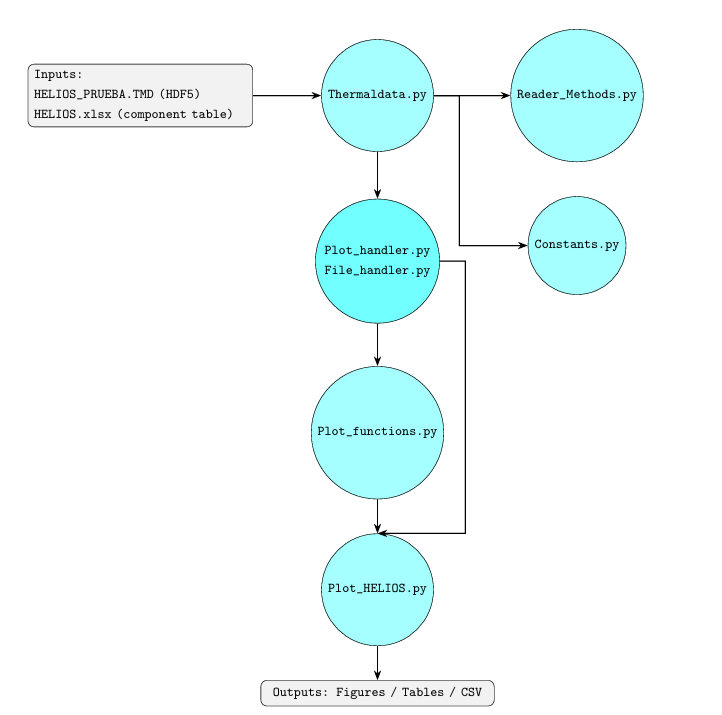
\includegraphics[width=0.78\textwidth]
    {Figures/03/arquitectura_HELIOS.png}
    \caption{Architecture of the initial post-processing implementation.
    Taken from \cite{tfg_carol}.}
    \label{fig:helios_previous_architecture}
\end{figure}

The architecture separates result reading, data organisation and 
representation. \texttt{Thermaldata.py} imports the HELIOS result file and 
the external component table, while the supporting modules handle data 
selection, file management and plotting. The interface is provided by 
\texttt{Plot\_HELIOS.py}, from which figures, tables and data files can be 
generated \cite{tfg_carol}.

This implementation is suitable for examining the thermal results of an individual
steady-state case. However, it does not provide complete post-processing of
transient results or allow several simulation cases to be loaded and compared
simultaneously. Extending the same structure to time-dependent results and
multiple cases requires changes to both data management and representation.

\section{Motivation for the Present Work}
\label{sec:project_motivation}

Transient simulations associate each calculated value with a specific
simulation time. The post-processing tools must preserve this correspondence
when results are selected, represented, and compared, particularly when
several components or interfaces are considered together.

During an orbital cycle, transitions between solar illumination and eclipse
and changes in internal dissipation produce variations in the thermal response
of the spacecraft. These variations must therefore be examined throughout the 
orbital cycle to determine when they occur and which elements are most affected.

Comparing simulation cases introduces an additional requirement. Spacecraft
thermal analyses may include several cases representing different
environmental and operating conditions. Processing them separately requires
equivalent elements to be selected again for every case and prevents their
direct comparison within the same representation. Managing cases associated
with the same thermal model together allows equivalent selections to be
applied and the differences between them to be calculated consistently.

For these reasons, the application is extended to process transient
results and manage several simulation cases associated with the same thermal
model. This allows equivalent components and interfaces to be compared
throughout the simulated period and the intervals in which the differences
between cases are most significant to be identified.
\cleardoublepage

\chapter{Theoretical Background} \label{ch:chapter_04}
\section{Thermal Control in Engineering}
In engineering applications, thermal control is decisive to optimize the 
performance of the system and its components, while keeping them within temperature limits. In some systems 
and elements, such as engines, electric components or aeroespace systems, the implementation of a \acrfull{tcs} 
is critical because thermal variations can produce a negative 
impact on their performance and structural safety \cite{th_handbook}.

Methods such as convection, conduction and radiation can be implemented on Earth's surface to study heat 
transfer phenomena. However, the lack of an atmosphere in space, limits heat transfer mechanisms to conduction 
in solids and thermal radiation into space \cite{spacethctrl}. 

The primary objective of a Spacecraft \acrshort{tcs} is to ensure that all onboard components operate within 
their specified temperature ranges during all mission 
phases, while minimizing resource consumption (mass and power)\cite{tcs_slides0}. 
This is achieved through a careful balance of internal heat dissipation and external environmental fluxes, utilizing 
both passive and active thermal control technologies \cite{th_handbook}.


Those aspects are critical because, unlike terrestrial applications, the space environment is characterized by extreme conditions, 
such as vacuum, a background temperature of 3K, and rapid, intense thermal cycling due to 
exposure to sunlight and Earth's shadow \cite{tcs_slides0,spacethctrl}.


Failure to comply with these thermal limits can lead to equipment malfunctions, accelerated material 
degradation, reduced reliability, structural damage from thermal cycling, or even catastrophic failure.

The objective of thermal control is to prevent those situations, ensuring operational reliability and 
enhancing the efficiency of the system \cite{hmt_f&a}. Some key requirements for 
the \acrshort{tcs} include \cite{tcs_slides1}:
\begin{itemize}[label={\scriptsize\raisebox{0.5ex}{\textbullet}}]
	\item Temperature Ranges: maintaining specific operational and survival temperature ranges 
	for components: electronics, batteries or infrared detectors
	\item Thermal Gradients and Stability: controlling temperature gradients and stability is essential 
	for high-precision systems such as cameras, optical benches, and CCD sensors to 
	avoid structural distortions and measurement errors
\end{itemize}
 
\section{Space Thermal Environment}

Spacecraft thermal control is a process of energy management in which environmental heating plays a major role 
and therefore, has a major impact in the spacecraft design. There is no convection in space due to the absence of an atmosphere,
being radiation the only possible method to dissipate heat in space. \newline
Nevertheless, heat conduction between the structure and the components of the spacecraft still occurs. \cite{th_handbook}

\section{Heat Transfer Mechanisms}

Heat can be defined as the form of energy that can be transferred from one system to another 
as a result of temperature difference. The science that deals with the determination of the rates of such 
energy transfers is heat transfer \cite{hmt_f&a}.
Conduction, convection and radiation are the fundamental mechanisms of heat transfer. However, as it is mentioned earlier,
there is no convection in space systems, leaving conduction and radiation as the predominant mechanisms. \cite{th_handbook}

% EJEMPLO DE COMO PONER UNA IMAGEN
%\begin{figure}[H]
%	\centering
%	
\includegraphics[width=100mm]{imag_07.png}
%	\caption{ Spectral distribution of the emissive power of a blackbody at different temperatures.
%The peak shifts to shorter wavelengths as temperature increases, according to Planck’s Law, \cite{heattransfer}} % Pie de imagen
%	\label{fig:001_01}
%\end{figure}

\subsection{Conduction Heat Transfer}

Heat transfer conduction is the mechanism by which thermal energy is transmitted 
through solids or between solids in contact due to the presence of a temperature gradient, without any 
macroscopic motion of the substance. This process is governed by microscopic interactions between 
particles and, in metallic materials, the transport of free electrons \cite{hmt_f&a}.

From a macroscopic perspective, heat conduction is described by Fourier’s law:
\begin{equation}
q = -k A \frac{dT}{dx}
\label{eq:Fourier}
\end{equation}

where: 
\begin{itemize}[label={\scriptsize\raisebox{0.5ex}{\textbullet}}]
	\item $q$ is the heat transfer rate (W) 
	\item $k$ is the thermal conductivity (W/mK) 
	\item $A$ is the cross-sectional area (m$^2$) 
	\item $\frac{dT}{dx}$ is the temperature gradient (K/m). 
\end{itemize}

The negative sign in the temperature gradient indicates that heat flows from regions of higher 
temperature to lower temperature \cite{hmt_f&a, spacethctrl}.

Under steady-state conditions and simple geometries, 
Fourier’s law can be integrated to obtain analytical expressions for heat transfer. 
For instance, in a plane wall with constant thermal conductivity, the heat flux is directly proportional to the temperature
difference between the boundaries and inversely proportional to the wall thickness \cite{hmt_f&a}. \newline
\autoref{fig:001_07} illustrates one-dimensional heat conduction through a flat wall, consistent with the
formulation of Fourier's law in \autoref{eq:Fourier}. 

\begin{figure}[H]
	\centering
	
\includegraphics[width=100mm]{imag_07.png}
	\caption{One-dimensional heat conduction accross the wall, with thickness $\Delta x$ ,whose surfaces are at 
temperatures  T1  and  T2  (T1  >  T2), respectively \cite{spacethctrl}} % Pie de imagen
	\label{fig:001_07}
\end{figure}

For more general cases involving spatial and temporal variations, the heat conduction process is 
governed by the heat diffusion equation, expressed in cartesian coordinates as:

\begin{equation}
\rho c_p \frac{\partial T}{\partial t} = \nabla \cdot (k \nabla T) + \dot{q}
\end{equation}

where $\rho$ is the density (kg/m$^3$), $c_p$ is the specific heat (J/kgK), 
and $\dot{q}$ represents internal heat generation per unit volume (W/m$^3$). 
This equation forms the basis for thermal modelling in both analytical and numerical approaches, 
including finite difference and nodal methods \cite{hmt_f&a, thermal_eng_man, ecss_man}.

An additional useful concept in conduction analysis is thermal resistance, which simplifies 
the study of heat transfer in complex systems. 
For a homogeneous layer, the conductive thermal resistance is defined as:

\begin{equation}
R_{cond} = \frac{L}{kA}
\end{equation}

where $L$ is the thickness of the material. \newline
In multilayer structures, individual resistances can be combined in series or parallel, allowing the overall 
heat transfer to be evaluated using an approach analogous to electrical circuits \cite{hmt_f&a}.

In the context of spacecraft thermal control, conduction plays a fundamental role in the 
internal redistribution of heat. Conductive paths are essential to transport heat generated 
by onboard components towards external radiative surfaces. Therefore, the design of conductive 
interfaces, material selection, and contact conductance are critical factors in ensuring proper 
thermal management \cite{spacethctrl, th_handbook, ecss_man}.

Furthermore, in thermal modelling tools such as ESATAN, conduction is 
typically represented through thermal conductances connecting discrete nodes within a network.
These conductances depend on material properties and geometry and are used to solve the energy balance 
equations governing the thermal behaviour of the system \cite{thermal_eng_man}.

\subsection{Radiation Heat Transfer}
%\begin{figure}[H]
%	\centering
%	
\includegraphics[width=100mm]{imag_07.png}
%	\caption{ Spectral distribution of the emissive power of a blackbody at different temperatures.
%The peak shifts to shorter wavelengths as temperature increases, according to Planck’s Law, \cite{heattransfer}} % Pie de imagen
%	\label{fig:001_01}
%\end{figure}
\section{Mathematical Modeling of Thermal Systems}

Mathematical modeling is essential to predict the thermal behavior of space systems and design
effective thermal control strategies. 

\subsection{Disadvantages of the Finite Element Method (FEM)}



\subsection{Lumped Parameter Method (LPM)}

The \acrfull{lpm} is a discretization technique that simplifies a continuous physical system 
into a finite number of discrete elements called nodes. 
The fundamental assumption is that each node is isothermal, meaning its temperature is uniform throughout its entire volume. 
This allows the system to be solved as a network of interconnected thermal resistances and 
capacitances, analogous to an electrical circuit, 
where temperature equates to voltage and heat flow to current flow. \cite{thermal_eng_man}

\autoref{fig:001_04} shows a simplified thermal system and its equivalent nodal network representation:

\begin{figure}[H]
	\centering
	
\includegraphics[width=130mm]{imag_04.png}
	\caption{Simplified heat transfer system and its corresponding thermal network \cite{lpm_elec}} % Pie de imagen
	\label{fig:001_04}
\end{figure}

The behaviour of the network can be described as a system of differential equations whose coefficients are grouped values of the nodes. The mathematical expression for the nodal energy balance equation is:

\begin{equation}
    C_i \frac{dT_i}{dt} = Q_i - \sum_{j=1}^{n} GL_{ij}(T_i - T_j) - \sum_{j=1}^{n} GR_{ij}(T_i^4 - T_j^4)
\end{equation}
where:

\begin{itemize}[label={\scriptsize\raisebox{0.5ex}{\textbullet}}]
	\item $C_i$ [J/K]: thermal capacitance of node $i$ ($m_i\ c_p,_i$); stores/releases heat as $T_i$ changes.  %El dolar se usa para ponerlo en formato formula

	\item $T_i$ [K]: temperature of node $i$.

	\item $t$ [s]: time.

	\item $GL_{ij}$ [W/K]: conductive conductance between nodes $i$ and $j$. The value is zero if there is not a conductive path.

	\item $GR_{ij}$ [$W/K^4$]: radiative coupling factor between $i$ and $j$ in the non-linear $T^4$ form; it embeds
$\sigma$, view factors and emissivities for diffuse–gray surfaces.

	\item $Q_i$ [W]: net heat source applied to node $i$ (internal dissipation, heaters, and absorbed external fluxes as modelled in the network).

	\item $\sum_{j=1}^n$: sum over all nodes $j$, which are thermally connected to $i$. The terms $GL_{ij}(T_i-T_j)$ and $GR_{ij}(T_i^4-T_j^4)$ contribute as inflow when the expression in parentheses is negative.
\end{itemize}


The discrete approximation simplifies the numerical solution of the thermal problem by reducing 
a continuous system, governed by differential equations, to a finite set of equations 
defined over a limited number of nodes. In steady-state conditions, this system becomes algebraic 
and can be solved using standard numerical techniques, whereas in transient analysis it remains a 
system of differential equations \cite{thermal_eng_man}.

Once the energy balance is defined for each node, the complete model is obtained by assembling 
all the equations into a coupled system. This system describes the temporal evolution of the nodal 
temperatures, taking into account both internal heat sources and the thermal interactions between nodes. \cite{thermal_eng_man}

In this framework, thermal systems are represented as networks of nodes connected through thermal 
conductances. These conductances account for the main heat transfer mechanisms, such as conduction 
through structural elements and radiation exchange between surfaces. Each node is characterised by 
its thermal capacitance and exchanges heat with the rest of the system, enabling the prediction of 
both steady-state and transient behaviour \cite{thermal_eng_man, spacethctrl}.

The accuracy of this method depends on the discretisation of the system. A reduced number of nodes 
may not capture the relevant temperature gradients, while an excessive number increases the 
computational cost without providing significant accuracy in the results. Therefore, the definition of 
the nodes represents a compromise between accuracy and efficiency. \cite{ecss_man}

Therefore, due to its balance between accuracy and computational cost, this method is widely used in spacecraft
thermal modelling and forms the basis of tools such as ESATAN-TMS. \cite{ecss_man}
%Therefore, this method has a wide range of applications in the aeroespace industry, such as the thermal modeling of satellites, 
%where a balance between accuracy and efficiency is required.

\section{Software and Advanced Methods for Thermal Simulation}

\section{Analytical Capabilities of ESATAN-TMS}




\cleardoublepage

\chapter[Thermal Model Development and Analysis Cases]
{Thermal Model Development in \\ ESATAN-TMS and Transient Analysis \\ Cases}
\label{ch:thermal_model}

The thermal model developed in \acrshort{esatan-tms} generates the results 
analysed throughout this work. It does not reproduce a particular flight 
design in full detail. Instead, it represents the main heat-transfer 
interactions with sufficient geometrical and physical detail to generate 
transient results and compare different cases. The same geometry, node 
hierarchy and thermal network are retained in every simulation, while the 
environmental and operating conditions are modified between cases.

The model contains the main body, two solar-panel wings, a camera, several 
internal electronic units, a battery, a radiator and \acrfull{mli}. Conductive 
and radiative couplings connect these elements, allowing temperatures and heat 
flows to be calculated throughout each simulation. The model follows the 
lumped-parameter formulation presented in 
\autoref{ch:theoretical_background} and implemented in 
\acrshort{esatan-tms} \cite{thermal_eng_man,esatan_user_man}.


\section{Model Development and Geometrical Configuration}
\label{sec:model_geometry}

The geometrical model is refined to represent the arrangement of the internal 
plates and equipment and the main conductive connections between them. This 
organisation also maintains a direct link between the physical elements and 
the node hierarchy used by the post-processing application.

The final internal configuration is shown from the $+Y$ and $-Y$ sides in 
Figure~\ref{fig:final_internal_model}. Both views show the 
distribution of the equipment across the structural plates and the different 
levels of the main body. The dissipative components represented in the model 
are the camera electronics, the battery, the \acrfull{obc}, the communications 
unit and the \acrfull{adcs}. Each unit is represented separately, allowing an 
individual internal heat load to be assigned and the corresponding temperature 
and heat exchanges to be analysed independently

The final external configuration is shown in
Figure~\ref{fig:final_external_model}. The main body presents a rectangular geometry 
and is divided into several surface nodes. Two solar-panel wings extend from 
opposite sides and are discretised independently. The camera assembly extends 
from the main body. Heat is rejected to space through the radiator, while the 
\acrshort{mli}-covered surfaces limit heat exchange with the external 
environment.

\begin{figure}[!htbp]
    \centering
    \phantomcaption

    \begin{subfigure}[c]{0.82\textwidth}
        \centering
        
\includegraphics[
            width=\linewidth,
            trim=0 45 0 45,
            clip
        ]{Image_02.png}
        \caption{Internal configuration viewed from the $+Y$ side.}
        \label{fig:internal_model_positive_y}
    \end{subfigure}
\end{figure}

\begin{figure}[!htbp]
    \ContinuedFloat
    \centering

    \begin{subfigure}[c]{0.72\textwidth}
        \centering
        
\includegraphics[
            width=\linewidth,
            trim=0 55 0 55,
            clip
        ]{Comp_disipativos.png}
        \caption{Internal configuration viewed from the $-Y$ side.}
        \label{fig:internal_model_negative_y}
    \end{subfigure}

    \caption{Internal configuration of the spacecraft thermal model viewed
    from opposite sides. The colours correspond to the geometry layer and do
    not represent temperatures.}
    \label{fig:final_internal_model}
\end{figure}

\begin{figure}[!htbp]
    \centering
    
\includegraphics[
        width=0.92\textwidth,
        trim=0 55 0 55,
        clip
    ]{Satelite.png}

    \caption{Final external configuration of the spacecraft thermal model in
    \acrshort{esatan-tms}. The colours correspond to the geometry layer and do
    not represent temperatures.}
    \label{fig:final_external_model}
\end{figure}

\FloatBarrier

\section{Thermal Model Hierarchy}
\label{sec:model_hierarchy}

The numerical nodes are grouped according to the physical elements they 
represent. This hierarchy consists of four levels:

\begin{itemize}
    \item \textbf{Level 0:} includes the complete \texttt{SAT\_AFM} model and 
    the \texttt{SPACE} boundary.

    \item \textbf{Level 1:} separates the main structure from the solar-panel 
    assembly.

    \item \textbf{Level 2:} divides the structure into the body, camera, 
    avionics and \acrshort{mli} groups.

    \item \textbf{Level 3:} contains the individual panels, structural plates, 
    camera elements and equipment units.
\end{itemize}

Each group is identified by a node range and a short label, giving a 
consistent naming system throughout the model. The \textit{Power} field 
indicates the equipment groups which have an internal heat load applied. 
The complete classification is given in 
\autoref{tab:subsystem-classification}.

% Uses packages already loaded in Tex_Files/packages.tex.

\begin{table}[H]
    \centering
    \caption{Thermal-model hierarchy and node identifiers.}
    \label{tab:subsystem-classification}

    \scriptsize
    \setlength{\tabcolsep}{2.5pt}
    \renewcommand{\arraystretch}{1.06}

    \begin{tabularx}{\textwidth}{
        |>{\raggedright\arraybackslash}X
        |c
        |>{\raggedright\arraybackslash}X
        |l
        |>{\raggedright\arraybackslash}X
        |c|
    }
        \hline
        \textbf{Group} &
        \textbf{Level} &
        \textbf{Parent} &
        \textbf{ID} &
        \textbf{Label} &
        \textbf{Power} \\
        \hline

        Space
        & 0 & None
        & \#99999
        & SPACE
        & False \\
        \hline

        SAT\_AFM
        & 0 & None
        & \#10000--75250
        & SAT\_AFM
        & False \\
        \hline

        STRUCTURE
        & 1 & SAT\_AFM
        & \#10000--51150
        & STR
        & False \\
        \hline

        SOLAR\_PANELS
        & 1 & SAT\_AFM
        & \#70000--75250
        & SP
        & False \\
        \hline

        BODY
        & 2 & STRUCTURE
        & \#10000--13650
        & STR\_BOD
        & False \\
        \hline

        CAMERA
        & 2 & STRUCTURE
        & \#40000--43750
        & STR\_CAM
        & False \\
        \hline

        AVIONICS
        & 2 & STRUCTURE
        & \#30000--35550
        & STR\_AV
        & False \\
        \hline

        MLI
        & 2 & STRUCTURE
        & \#50000--51150
        & STR\_MLI
        & False \\
        \hline

        SOLAR\_PANEL\_1
        & 3 & SOLAR\_PANELS
        & \#70000--72550
        & SP\_1
        & False \\
        \hline

        SOLAR\_PANEL\_2
        & 3 & SOLAR\_PANELS
        & \#73000--75250
        & SP\_2
        & False \\
        \hline

        BODY\_PANEL
        & 3 & BODY
        & \#10000--11150
        & STR\_BOD\_P
        & False \\
        \hline

        BODY\_PLATE\_INF
        & 3 & BODY
        & \#12000--12550
        & STR\_BOD\_PLI
        & False \\
        \hline

        BODY\_PLATE\_MED
        & 3 & BODY
        & \#12600--13050
        & STR\_BOD\_PLM
        & False \\
        \hline

        BODY\_PLATE\_SUP
        & 3 & BODY
        & \#13100--13650
        & STR\_BOD\_PLS
        & False \\
        \hline

        CAMERA\_BASE
        & 3 & CAMERA
        & \#40000--40450
        & STR\_CAM\_BASE
        & False \\
        \hline

        CAMERA\_ELEC
        & 3 & CAMERA
        & \#40500--41050
        & STR\_CAM\_ELEC
        & True \\
        \hline

        CAMERA\_LENS
        & 3 & CAMERA
        & \#41500--42150
        & STR\_CAM\_LENS
        & False \\
        \hline

        CAMERA\_CYL
        & 3 & CAMERA
        & \#42500--43550
        & STR\_CAM\_CYL
        & False \\
        \hline

        BATTERY
        & 3 & AVIONICS
        & \#30000--30550
        & STR\_AV\_BAT
        & True \\
        \hline

        OBC\_BOX
        & 3 & AVIONICS
        & \#31000--31550
        & STR\_AV\_OBC
        & True \\
        \hline

        COMMS\_BOX
        & 3 & AVIONICS
        & \#32000--32550
        & STR\_AV\_COM
        & True \\
        \hline

        ADCS\_UNIT
        & 3 & AVIONICS
        & \#33000--33550
        & STR\_AV\_ADCS
        & True \\
        \hline

        RADIATOR
        & 3 & AVIONICS
        & \#34000--35550
        & STR\_AV\_RAD
        & False \\
        \hline

        MLI\_PANELS
        & 3 & MLI
        & \#50000--51150
        & STR\_MLI\_P
        & False \\
        \hline
    \end{tabularx}
\end{table}

\begin{figure}[H]
    \centering
    \phantomcaption

    \begin{subfigure}[c]{0.78\textwidth}
        \centering
        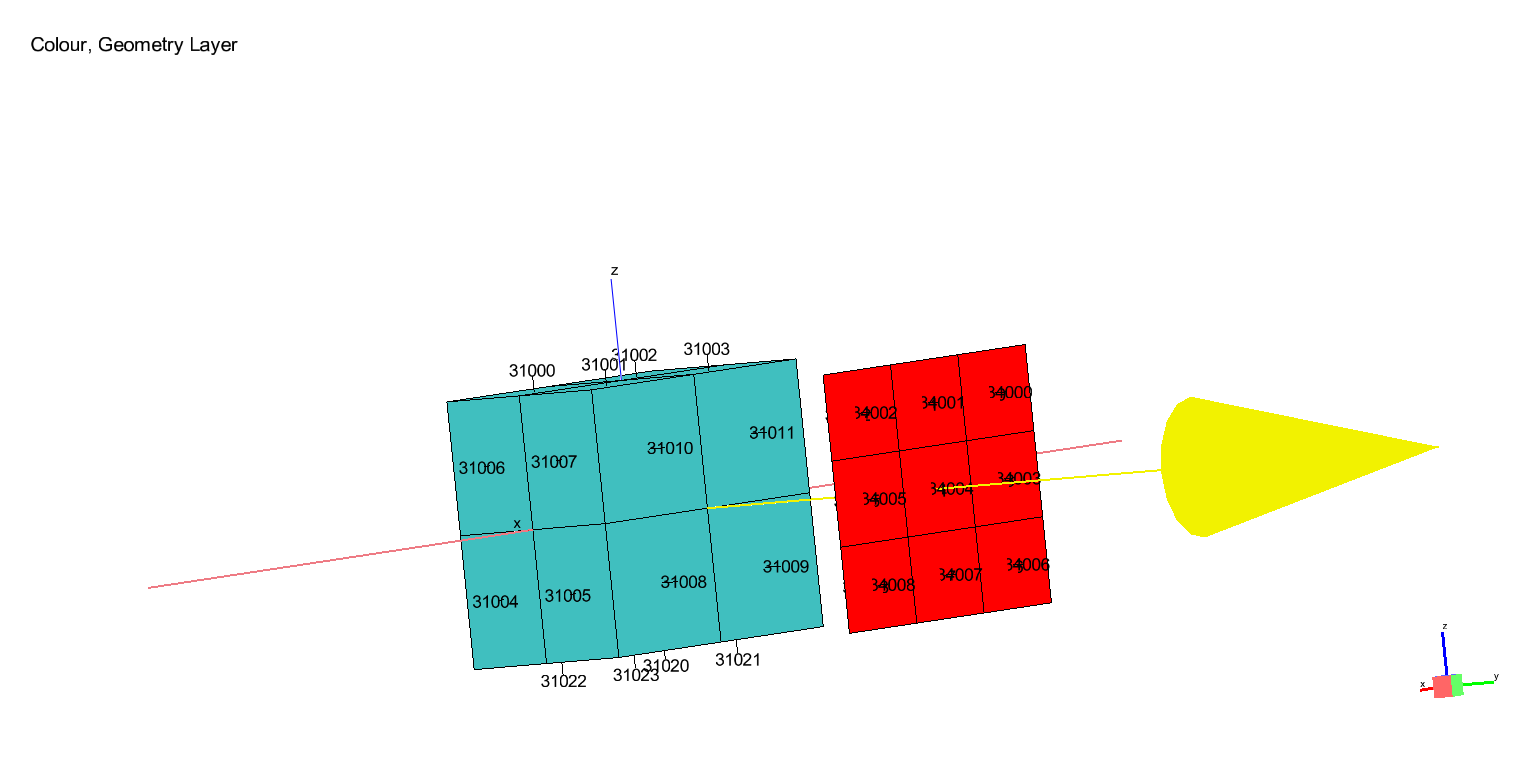
\includegraphics[width=\linewidth]
        {Figures/05/OBC_Rad_nodes.png}
        \caption{First view of the OBC and radiator nodal numbering.}
        \label{fig:obc_radiator_nodes_a}
    \end{subfigure}
\end{figure}

\begin{figure}[H]
    \ContinuedFloat
    \centering

    \begin{subfigure}[c]{0.78\textwidth}
        \centering
        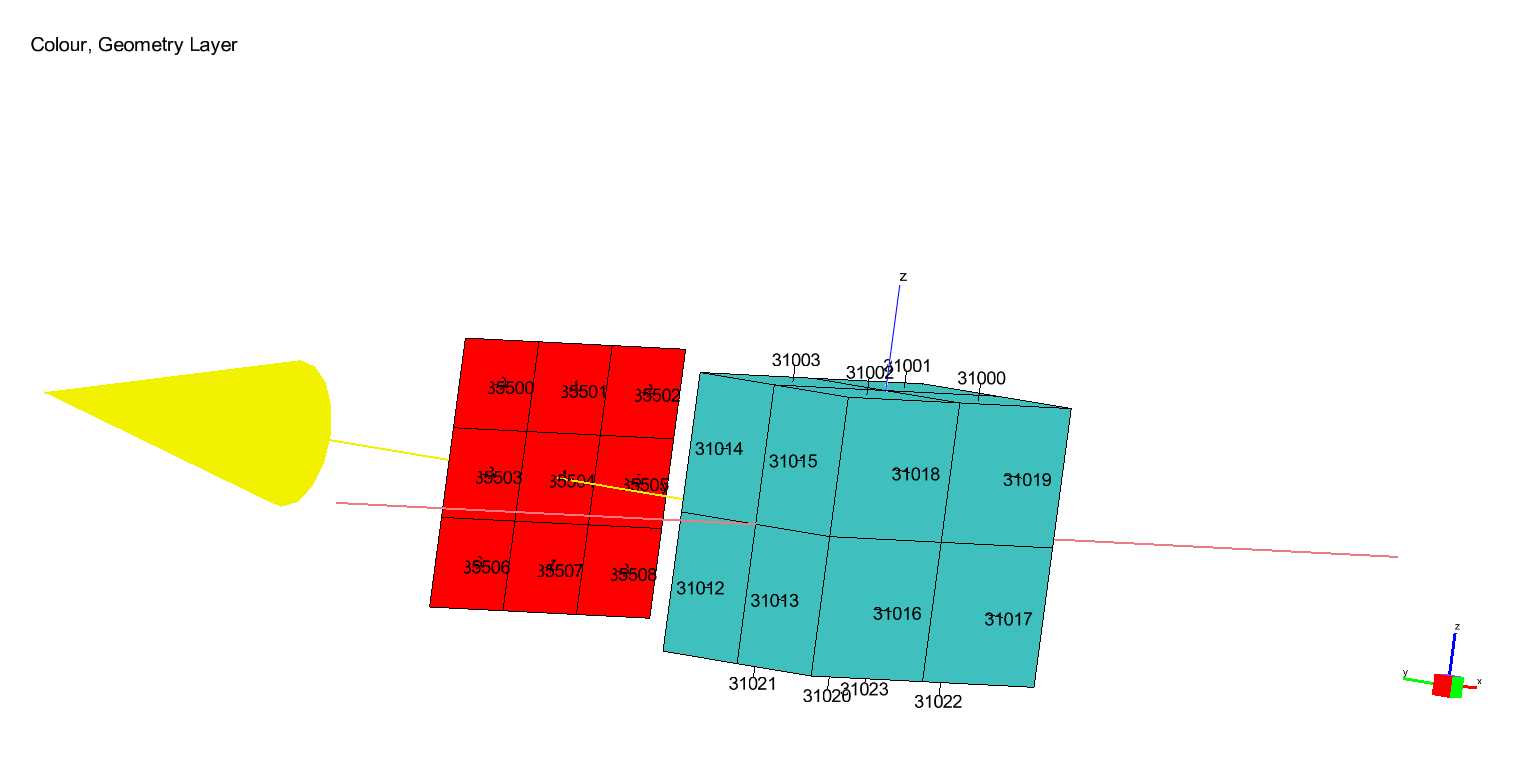
\includegraphics[width=\linewidth]
        {Figures/05/OBC_Rad_nodes2.png}
        \caption{Opposite view of the OBC and radiator nodal numbering.}
        \label{fig:obc_radiator_nodes_b}
    \end{subfigure}

    \caption{Example of nodal numbering for the OBC and adjacent radiator
    surfaces, shown from opposite sides. The figure illustrates the node
    ranges listed in Table~\ref{tab:subsystem-classification}.}
    \label{fig:obc_radiator_nodes}
\end{figure}

\section{Material and Surface Properties}
\label{sec:model_properties}

The temperature response of each geometrical element depends on the 
assigned bulk material and the thermo-optical properties of the surfaces. 
Thermal conductivity, density and specific heat capacity determine 
heat conduction and energy storage, while the surface properties govern the 
interaction with solar and infrared radiation. The same definitions are used 
in all analysis cases. Consequently, changes in the calculated results are 
associated with the environmental and operating inputs rather than with 
modifications to the model.


\subsection{Bulk Properties}
\label{subsec:bulk_properties}

The geometrical elements use four material definitions. Aluminium 6061 is 
assigned to the main structural panels, internal plates and equipment 
housings. Gallium arsenide represents the solar-cell elements, while a 
separate optical material is used for the camera lens. The 
\acrshort{mli} foil has an independent definition whose conductivity is set 
to zero. This prevents the geometrical shell from introducing a 
solid-conduction connection, while the intended couplings are defined 
explicitly in the thermal network.

The conductivity, specific heat capacity and density assigned to each material 
are listed in \autoref{tab:material-properties}. 
Figure~\ref{fig:conductivity_distribution} shows only the conductivity 
distribution, using two opposite views to cover the complete geometry. This 
allows the assignments to the structure, solar cells, camera and 
\acrshort{mli} surfaces to be checked.

% Uses packages already loaded in Tex_Files/packages.tex.

\begin{table}[H]
    \centering
    \caption{Material properties used in the thermal model.}
    \label{tab:material-properties}
    
    \small
    \setlength{\tabcolsep}{6pt}
    \renewcommand{\arraystretch}{1.12}
    \resizebox{0.7\textwidth}{!}{%
        \begin{tabular}{|l|c|c|c|}
            \hline
            \textbf{Name} &
            \(\boldsymbol{k}\,[\mathrm{W\,m^{-1}\,K^{-1}}]\) &
            \(\boldsymbol{c_p}\,[\mathrm{J\,kg^{-1}\,K^{-1}}]\) &
            \(\boldsymbol{\rho}\,[\mathrm{kg\,m^{-3}}]\) \\
            \hline

            Al\_6061 & 160 & 900 & 2700 \\
            \hline

            GaAs & 55 & 1000 & 5300 \\
            \hline

            Glass & 59 & 310 & 5330 \\
            \hline

            MLI\_foil & 0 & 900 & 300 \\
            \hline
        \end{tabular}
    }
\end{table}

\par\addvspace{32mm}

\begin{figure}[H]
    \centering
    \phantomcaption

        \begin{subfigure}[c]{0.8\textwidth}
        \centering
        
\includegraphics[
            width=\linewidth,
            trim=0 8 0 120,
            clip
        ]{thermal_conductivity2.png}
        \caption{View from the side $+Y$.}
        \label{fig:conductivity_distribution_opposite}
    \end{subfigure}
\end{figure}

\begin{figure}[H]
    \ContinuedFloat
    \centering

    \begin{subfigure}[c]{0.7\textwidth}
        \centering
        
\includegraphics[
            width=\linewidth,
            trim=0 8 0 120,
            clip
        ]{thermal_conductivity.png}
        \caption{View from side $-Y$.}
        \label{fig:conductivity_distribution_view_a}
    \end{subfigure}

    \caption{Thermal conductivity distribution over the final spacecraft
    model, viewed from opposite sides.}
    \label{fig:conductivity_distribution}
\end{figure}

\FloatBarrier


\subsection{Thermo-optical Properties}
\label{subsec:thermo_optical_properties}

The surface definitions are assigned according to the function of each 
element. Anodised aluminium is used on selected structural surfaces, while 
black paint is applied to the internal equipment. An \acrfull{osr} defines the 
radiator surface, and the solar cells use a separate coating definition. The 
external \acrshort{mli} is represented by Kapton coated with 
\acrfull{ito}, while independent properties are assigned to the internal 
\acrshort{mli} and the infrared lens.

The solar and infrared bands are defined separately. For each surface, the 
model specifies absorptivity or emissivity, transmissivity and the specular 
and diffuse components of reflectivity. Within each band, these coefficients 
are defined so that the corresponding energy fractions sum to unity.

The adopted solar absorptivity and infrared emissivity values are consistent 
with representative measurements compiled for black coatings, anodised 
aluminium, solar cells, optical solar reflectors and Kapton films 
\cite{kauder2005coatings}. These data are used as 
reference values, since a single nominal definition 
is assigned to each surface in the model. The complete set of properties is summarised in
\autoref{tab:thermo-optical-properties}.
% Source locations: printed pages 40, 43, 46 and 48;
% PDF pages 46, 49, 52 and 54.

% Uses packages already loaded in Tex_Files/packages.tex.

\begin{table}[H]
    \centering
    \caption{Thermo-optical coating properties used in the thermal model.}
    \label{tab:thermo-optical-properties}

    \setlength{\tabcolsep}{3pt}
    \renewcommand{\arraystretch}{1.15}
    
    \resizebox{0.6\textwidth}{!}{%
        \begin{tabular}{|l|*{8}{c|}}
            \hline
            \multirow{2}{*}{\textbf{Name}} &
            \multicolumn{4}{c|}{\textbf{Infrared}} &
            \multicolumn{4}{c|}{\textbf{Solar}} \\
            \cline{2-9}

            &
            \(\boldsymbol{\varepsilon}\) &
            \(\boldsymbol{\tau}\) &
            \(\boldsymbol{\rho_{\mathrm{spec}}}\) &
            \(\boldsymbol{\rho_{\mathrm{diff}}}\) &
            \(\boldsymbol{\alpha}\) &
            \(\boldsymbol{\tau}\) &
            \(\boldsymbol{\rho_{\mathrm{spec}}}\) &
            \(\boldsymbol{\rho_{\mathrm{diff}}}\) \\
            \hline

            Al anodized
            & 0.6 & 0 & 0 & 0.4
            & 0.2 & 0 & 0 & 0.8 \\
            \hline

            Black paint
            & 0.9 & 0 & 0 & 0.1
            & 0.9 & 0 & 0 & 0.1 \\
            \hline

            OSR
            & 0.8 & 0 & 0.2 & 0
            & 0.08 & 0 & 0.92 & 0 \\
            \hline

            Solar cells
            & 0.75 & 0 & 0 & 0.25
            & 0.75 & 0 & 0 & 0.25 \\
            \hline

            IR lens
            & 0.1 & 0.9 & 0 & 0
            & 0.5 & 0 & 0 & 0.5 \\
            \hline

            Kapton ITO
            & 0.8 & 0 & 0 & 0.2
            & 0.5 & 0 & 0 & 0.5 \\
            \hline

            MLI\_int
            & 0.2 & 0 & 0 & 0.8
            & 0.2 & 0 & 0 & 0.8 \\
            \hline
        \end{tabular}
    }   
\end{table}

The solar absorptivity and reflectivity distributions are presented in
Figures~\ref{fig:solar_absorptivity_distribution}
and~\ref{fig:solar_reflectivity_distribution}. Higher absorptivity is assigned 
to the solar cells and black-painted surfaces, whereas the radiator 
\acrshort{osr} has the lowest value. The reflectivity maps show the 
corresponding distribution of reflected solar energy. Two opposite views are 
included for each property so that the assignments can be checked over the 
complete geometry.

\begin{figure}[!htbp]
    \centering
    \phantomcaption

    \begin{subfigure}[c]{1.0\textwidth}
        \centering
        
\includegraphics[width=\linewidth]
        {solar_absorptivity.png}
        \caption{View from one side.}
        \label{fig:solar_absorptivity_distribution_view_a}
    \end{subfigure}
\end{figure}

\begin{figure}[!htbp]
    \ContinuedFloat
    \centering

    \begin{subfigure}[c]{1.0\textwidth}
        \centering
        
\includegraphics[width=\linewidth]
        {solar_absorptivity2.png}
        \caption{View from the opposite side.}
        \label{fig:solar_absorptivity_distribution_opposite}
    \end{subfigure}

    \caption{Solar absorptivity distribution over the final spacecraft
    model, viewed from opposite sides.}
    \label{fig:solar_absorptivity_distribution}
\end{figure}

\begin{figure}[!htbp]
    \centering
    \phantomcaption

    \begin{subfigure}[c]{1.0\textwidth}
        \centering
        
\includegraphics[width=\linewidth]
        {solar_reflectivity.png}
        \caption{View from one side.}
        \label{fig:solar_reflectivity_distribution_view_a}
    \end{subfigure}
\end{figure}

\begin{figure}[!htbp]
    \ContinuedFloat
    \centering

    \begin{subfigure}[c]{1.0\textwidth}
        \centering
        
\includegraphics[width=\linewidth]
        {solar_reflectivity2.png}
        \caption{View from the opposite side.}
        \label{fig:solar_reflectivity_distribution_opposite}
    \end{subfigure}

    \caption{Solar reflectivity distribution over the final spacecraft
    model, viewed from opposite sides.}
    \label{fig:solar_reflectivity_distribution}
\end{figure}

\FloatBarrier

The infrared emissivity and reflectivity distributions are shown in
Figures~\ref{fig:infrared_emissivity_distribution}
and~\ref{fig:infrared_reflectivity_distribution}. High emissivity is assigned 
to the black-painted surfaces and the radiator, promoting radiative heat 
exchange. Lower values are used for the internal \acrshort{mli} and the camera 
lens, which also includes infrared transmissivity. These assignments determine 
the radiative exchange between internal elements and the rejection of heat 
from the external surfaces.

\begin{figure}[!htbp]
    \centering
    \phantomcaption

    \begin{subfigure}[c]{1.0\textwidth}
        \centering
        
\includegraphics[width=\linewidth]
        {infrarred_emmisivity.png}
        \caption{View from one side.}
        \label{fig:infrared_emissivity_distribution_view_a}
    \end{subfigure}
\end{figure}

\begin{figure}[!htbp]
    \ContinuedFloat
    \centering

    \begin{subfigure}[c]{1.0\textwidth}
        \centering
        
\includegraphics[width=\linewidth]
        {infrarred_emmisivity2.png}
        \caption{View from the opposite side.}
        \label{fig:infrared_emissivity_distribution_opposite}
    \end{subfigure}

    \caption{Infrared emissivity distribution over the final spacecraft
    model, viewed from opposite sides.}
    \label{fig:infrared_emissivity_distribution}
\end{figure}

\begin{figure}[!htbp]
    \centering
    \phantomcaption

    \begin{subfigure}[c]{1.0\textwidth}
        \centering
        
\includegraphics[width=\linewidth]
        {infrarred_reflectivity.png}
        \caption{View from one side.}
        \label{fig:infrared_reflectivity_distribution_view_a}
    \end{subfigure}
\end{figure}

\begin{figure}[!htbp]
    \ContinuedFloat
    \centering

    \begin{subfigure}[c]{1.0\textwidth}
        \centering
        
\includegraphics[width=\linewidth]
        {infrarred_reflectivity2.png}
        \caption{View from the opposite side.}
        \label{fig:infrared_reflectivity_distribution_opposite}
    \end{subfigure}

    \caption{Infrared reflectivity distribution over the final spacecraft
    model, viewed from opposite sides.}
    \label{fig:infrared_reflectivity_distribution}
\end{figure}

\FloatBarrier


\section{Nodal Discretisation and Thermal Network Definition}
\label{sec:thermal_network_definition}

The geometrical model is divided into nodes according to the spatial 
resolution required for the analysis. Large external elements, including the 
body panels and solar-panel wings, are represented by several nodes to capture 
local temperature differences and variations in the absorbed environmental loads. 
Internal plates and equipment units are also discretised separately to 
reproduce the main heat-transfer paths through the structure.

Each capacitive node is assigned a material, mass and specific heat capacity.
Following this nodal division, the conductive network represents 
heat transfer through the structure and between the internal equipment 
and supporting plates. Most conductive 
paths correspond to physical contacts included in the geometry. When a physical 
connection is not represented geometrically, an additional conductor is defined. 
This is the case for the thermal link between the \acrshort{obc} and the radiator, 
which is included without adding unnecessary geometrical detail.

The radiative network represents exchange between the relevant surfaces and with the 
deep-space boundary.

Internal heat loads are applied to the nodes representing the dissipative equipment. 
The values assigned in each transient case are summarised in 
Table~\ref{tab:internal_heat_loads}. The battery load is defined separately
for eclipse and non-eclipse intervals.

\begin{table}[htbp]
    \centering
    \caption{Internal heat loads applied in the selected transient cases.}
    \label{tab:internal_heat_loads}

    \small
    \setlength{\tabcolsep}{5pt}
    \renewcommand{\arraystretch}{1.15}

    \begin{tabularx}{\textwidth}{
        |>{\raggedright\arraybackslash}X
        |*{3}{>{\centering\arraybackslash}p{0.19\textwidth}|}
    }
        \hline
        \multirow{2}{*}{\textbf{Component}} &
        \multicolumn{3}{c|}{\textbf{Applied power (W)}} \\
        \cline{2-4}

        &
        \textbf{Nominal} &
        \textbf{Hot} &
        \textbf{Cold} \\
        \hline

        Camera electronics
        & 2.00
        & 3.50
        & 0.00 \\
        \hline

        Battery, outside eclipse
        & 1.50
        & 2.06
        & 0.375 \\
        \hline

        Battery, during eclipse
        & 10.00
        & 13.75
        & 2.50 \\
        \hline

        \acrshort{obc}
        & 4.00
        & 5.00
        & 2.00 \\
        \hline

        Communications unit
        & 3.00
        & 4.50
        & 0.50 \\
        \hline

        \acrshort{adcs}
        & 2.00
        & 3.50
        & 0.50 \\
        \hline
    \end{tabularx}
\end{table}

The node definitions and conductive and radiative couplings remain unchanged in all 
transient cases. Only the environmental conditions and internal heat loads 
are modified as requires for each case. Consequently, each node and thermal coupling 
represents the same physical element in every exported result file, allowing direct 
comparison between cases.


\section{Orbital Environment and Radiative Cases}
\label{sec:radiative_cases}

The orbital environment defines the external radiative conditions applied to
the model. Direct solar radiation, planetary albedo and planetary infrared
emission are included as external heat inputs \cite{ecss_st_10_04c}. Energy
emitted by the external surfaces towards deep space is also considered. These
exchanges are represented through the orbital and radiative models of
\acrshort{esatan-tms} and provide the boundary conditions used in the
transient simulations \cite{thermal_eng_man}.

Three radiative cases are selected: \texttt{rad\_nominal},
\texttt{rad\_hot\_operational} and
\texttt{rad\_cold\_operational}. The same geometry and surface properties are
retained in all three cases, while the environmental parameters and eclipse
duration differ between them. For the radiative calculation, each orbital
revolution is divided into 24 positions separated by \(15^{\circ}\). This
common angular sampling allows the incident loads to be evaluated consistently
throughout the orbit and included in the transient solution.

Figure~\ref{fig:nominal_orbit_positions} shows the orbital configuration of
the nominal case. The spacecraft positions illustrate the discretisation used
for the radiative calculation. The green segment represents the portion
outside eclipse, whereas the red segment identifies the eclipse interval.

\begin{figure}[H]
    \centering
    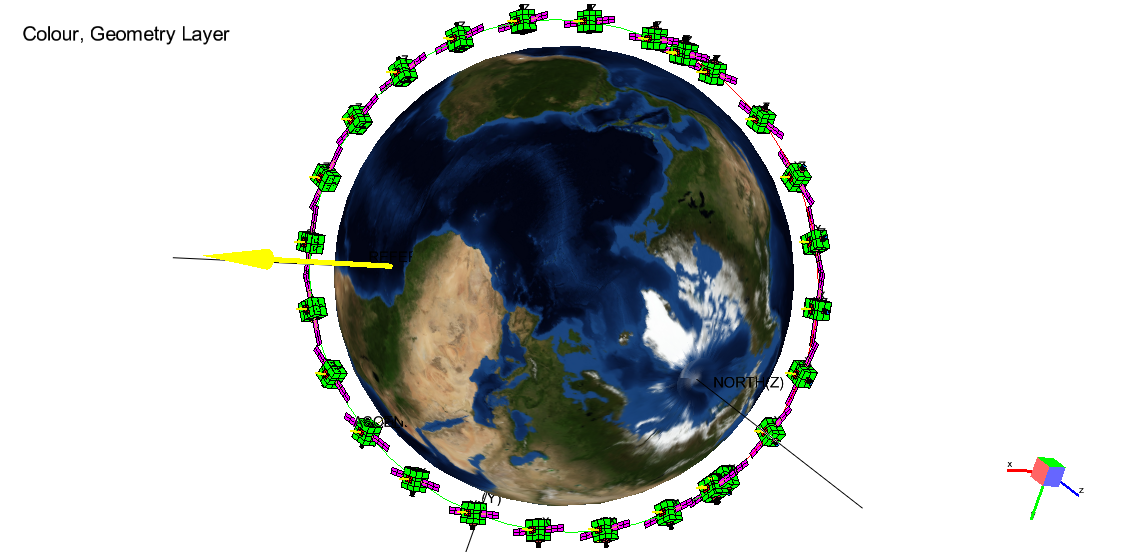
\includegraphics[width=1.0\textwidth]
    {Figures/05/nominal_orbit_positions.png}
    \caption{Nominal orbital configuration and the 24 positions used for the
    radiative calculation. The green segment represents the portion outside
    eclipse, while the red segment indicates the eclipse interval.}
    \label{fig:nominal_orbit_positions}
\end{figure}

The \texttt{rad\_nominal} case provides the reference environment.
\texttt{rad\_hot\_operational} combines a higher external heat input with a
shorter eclipse, whereas \texttt{rad\_cold\_operational} combines a lower
input with a longer eclipse.

These environments provide clearly differentiated conditions for comparing
the hot and cold responses with the nominal case without modifying the
physical model. They are selected for the analyses performed in this work and
do not cover every condition expected during a flight mission.

\section{Transient Analysis Cases}
\label{sec:transient_cases}

\subsection{Definition of Analysis Cases}
\label{subsec:analysis_case_definition}

Three transient simulations are selected for the final analysis: nominal, hot
and cold. The nominal case provides the reference response, while the hot and
cold cases represent higher and lower external heat inputs, respectively.
Different equipment loads are also assigned according to the operating
conditions defined for each simulation. Their purpose is summarised in
Table~\ref{tab:transient_cases}.

\begin{table}[htbp]
    \centering
    \caption{Transient cases selected from the common thermal model.}
    \label{tab:transient_cases}

    \small
    \setlength{\tabcolsep}{6pt}
    \renewcommand{\arraystretch}{1.15}

    \begin{tabularx}{\textwidth}{
        |>{\raggedright\arraybackslash}p{0.17\textwidth}
        |>{\raggedright\arraybackslash}p{0.27\textwidth}
        |>{\raggedright\arraybackslash}X|
    }
        \hline
        \textbf{Case} &
        \textbf{Radiative case} &
        \textbf{Purpose} \\
        \hline

        Nominal &
        \texttt{rad\_nominal} &
        Reference response used for comparison with the hot and cold cases. \\
        \hline

        Hot &
        \texttt{rad\_hot\_operational} &
        Response under higher external heat input and a shorter eclipse. \\
        \hline

        Cold &
        \texttt{rad\_cold\_operational} &
        Response under lower external heat input and a longer eclipse. \\
        \hline
    \end{tabularx}
\end{table}

The same geometry, materials, surface properties, node labels, hierarchy and
thermal couplings are retained in all three simulations. Only the radiative
environment and internal heat loads change between cases. Equivalent nodes and
variables therefore retain the same physical meaning, allowing the hot and
cold results to be compared directly with the nominal case.


\subsection{Solver Configuration and Temporal Sampling}
\label{subsec:solver_sampling}

The \textit{Solution Control} configuration applied to the three analysis
cases is shown in Figure~\ref{fig:solver_execution_block}.

\begin{figure}[htbp]
    \centering
    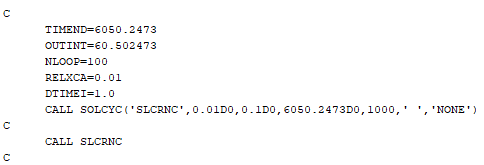
\includegraphics[width=0.9\textwidth]
    {Figures/05/solver_execution_block.png}
    \caption{\textit{Solution Control} execution block used to obtain cyclic
    convergence and calculate the final transient orbital period in
    \acrshort{esatan-tms}.}
    \label{fig:solver_execution_block}
\end{figure}

\begin{samepage}

The same numerical settings are used in all three simulations. The transient
solution is calculated using the Crank--Nicolson method. Before the final
results are exported, \texttt{SOLCYC} repeats the orbital period until the
maximum difference between the initial and final nodal temperatures is below
\(0.01\,^{\circ}\mathrm{C}\). A maximum of 1000 cycles is allowed. The
converged temperature field is then used as the initial condition for the
orbital period retained for analysis.

Each exported simulation covers \(6050.247\,\mathrm{s}\) and contains 101
output instants separated by approximately \(60.50\,\mathrm{s}\). This common
time basis records the main changes in the applied loads and allows values
from different cases to be compared at equivalent points of the orbit.

\end{samepage}


\section{Thermal Model Verification}
\label{sec:thermal_model_verification}

Verification is performed throughout model development using visual and
numerical checks. The material and surface-property maps are inspected to
identify missing or incorrectly assigned faces. The node hierarchy is 
compared with the physical arrangement to confirm that the external panels,
internal plates and equipment units belong to the correct model groups.

The conductive and radiative networks are reviewed to identify isolated nodes,
missing links and unintended heat-transfer paths. Nodal energy balances are
examined to detect inconsistent loads or exchanges. Finally, the exported
results are checked to confirm that every selected case satisfies the required
cyclic-convergence criterion.

These checks confirm the internal consistency of the model but do not validate it
against experimental data. No corresponding flight hardware or thermal-vacuum
test data are available for comparison. The conclusions are therefore limited
to the behaviour predicted by the model under the defined environmental and
operating conditions.


\section{Simulation Results Export in TMD Format}
\label{sec:tmd_export}

After each simulation is completed, the result set obtained for each case is exported from
\acrshort{esatan-tms} as a separate \texttt{.TMD} file. Each file stores the
time vector and the nodal quantities selected for post-processing, including
temperatures, applied loads, absorbed environmental loads, and conductive and
radiative heat flows. Node numbers and labels are preserved during export,
allowing each variable to be associated with the corresponding group in the
external hierarchy spreadsheet.

The structural and temporal dimensions shared by the three result files are
summarised in Table~\ref{tab:tmd_summary}. The nominal, hot and cold files
retain the same node and conductor structure and cover a common time
interval.

Together, the three files form the dataset used for the transient and
multi-case analyses. Their common structure allows equivalent variables to
be represented at the same orbital instants and compared directly with
respect to the nominal case.

\begin{table}[H]
    \centering
    \caption{Structural and temporal characteristics of the exported
        \texttt{.TMD} files.}
    \label{tab:tmd_summary}
    \small
    \setlength{\tabcolsep}{8pt}
    \renewcommand{\arraystretch}{1.15}

    \begin{tabularx}{0.76\textwidth}{|X|c|}
        \hline
        Total thermal nodes per file
        & 284 \\
        \hline

        Capacitive nodes
        & 282 \\
        \hline

        Boundary nodes
        & 1 \\
        \hline

        Inactive nodes
        & 1 \\
        \hline

        Linear conductors, \(G^{L}\)
        & 597 \\
        \hline

        Radiative conductors, \(G^{R}\)
        & 3292 \\
        \hline

        Time interval
        & \(6050.247\,\mathrm{s}\) \\
        \hline

        Output instants per file
        & 101 \\
        \hline

        Approximate output time step
        & \(60.502\,\mathrm{s}\) \\
        \hline
    \end{tabularx}
\end{table}

The 101 output instants correspond to the temporal sampling of the transient
solution and should not be confused with the 24 orbital positions used in the
radiative calculation. For each nodal variable, one file therefore contains
\(284 \times 101 = 28\,684\) values before the conductor results and remaining
nodal quantities are considered.

The absorbed solar loads calculated for the solar panels are also retained in
the exported data. These values are used as inputs for the
electrical-generation and battery calculations. This processing is
performed independently and does not modify the \acrshort{esatan-tms}
solution.

The three \texttt{.TMD} files and the hierarchy spreadsheet form the input
dataset used by the Python application to read, organise and compare the
results.
\cleardoublepage

\chapter[Multi-Case Post-Processing Tool]
{Development of the Multi-Case\\Post-Processing Tool}
\label{ch:multicase_tool}

\section{Starting Point and Development Scope}
\label{sec:development_scope}

\section{Application Architecture and Data Flow}
\label{sec:application_architecture}

\section{Multi-Case Loading and Data Management}
\label{sec:multicase_loading}

\section{Model Hierarchy, Selection and Case Comparison}
\label{sec:hierarchy_case_comparison}


\section{Model Inspection and Instantaneous Flow Visualisation}
\label{sec:model_inspection_visualisation}

\section{Saving, Restoring and Exporting Analyses}
\label{sec:analysis_management}
\cleardoublepage

\chapter[Transient Thermal Analysis]
{Transient Thermal Analysis\\and Multi-Case Comparison}
\label{ch:transient_analysis}

\section{Transient Data Processing}
\label{sec:transient_data_processing}

\section{Temperature and Thermal-Load Evolution}
\label{sec:thermal_histories}

\section{Interface Temperature-Difference Analysis}
\label{sec:interface_temperature_analysis}

\subsection{Interfaces between Model Components}
\label{subsec:component_interfaces}

\subsection{Variation over Selected Time Intervals}
\label{subsec:temperature_time_intervals}

\section{Thermal Summary Tables}
\label{sec:thermal_summary_tables}

\section[Heat-Flow Evolution]
{Conductive and Radiative Heat-Flow Evolution}
\label{sec:heat_flow_evolution}

\section{Thermal Energy and Summary Tables}
\label{sec:thermal_energy_summary}
\cleardoublepage

\chapter[Electrical Power Balance and Battery Model]
{Electrical Power Balance\\and Battery Model}
\label{ch:electrical_battery_analysis}

The \texttt{Energy balance} tab extends the thermal post-processing workflow
with a separate electrical calculation. The module first uses the solar load
exported by \acrshort{esatan-tms} to estimate the power generated by the solar
cells. It then obtains the electrical demand from the internal dissipations of
the selected equipment and applies the resulting power surplus or deficit to a
configurable lithium-ion battery model.

All operations take place after the thermal solution. The application reads
$Q_S$, $Q_I$ and the required temperature histories from the imported
\texttt{.TMD} file, but it does not modify those data or return any electrical
quantity to \acrshort{esatan-tms}. The thermal and electrical calculations
therefore remain one-way coupled: the solved thermal case supplies the inputs,
and the Python module derives solar generation, electrical demand, battery
state and operating limits.

The workflow contains two consecutive stages. The first converts the selected
solar-panel result into $Q_{S,\mathrm{elec}}$ and builds
$Q_{\mathrm{load}}$. The second uses both histories, together with the
battery temperature and the configurable cell parameters, to calculate stored
energy, state of charge, terminal voltage, charge and discharge currents,
losses and operating phases.


\section{Solar-to-Electrical Power Conversion}
\label{sec:solar_electrical_conversion}

\subsection{Conversion Method}
\label{subsec:solar_conversion_method}

The selected solar-panel group provides the absorbed solar load $Q_S(t)$. In
the adopted thermo-electrical formulation, the incident solar power
$Q_{S,i}(t)$ divides into a thermal fraction and an electrical fraction. The
solar absorptivity $\alpha$ describes the total fraction retained by the solar
cells, while the electrical conversion efficiency $\eta(t)$ defines the part
converted into electrical power. The effective thermal absorptivity becomes

\begin{equation}
    \alpha_{\mathrm{th}}(t)
    =
    \alpha-\eta(t).
    \label{eq:solar_effective_absorptivity}
\end{equation}

The thermal load exported for the selected group follows

\begin{equation}
    Q_S(t)
    =
    \left[\alpha-\eta(t)\right]Q_{S,i}(t).
    \label{eq:solar_thermal_load_conversion}
\end{equation}

The application therefore reconstructs the incident power from

\begin{equation}
    Q_{S,i}(t)
    =
    \frac{Q_S(t)}{\alpha-\eta(t)},
    \label{eq:solar_incident_power_reconstruction}
\end{equation}

and calculates the electrical contribution as

\begin{equation}
    Q_{S,\mathrm{elec}}(t)
    =
    \eta(t)Q_{S,i}(t)
    =
    \frac{\eta(t)}{\alpha-\eta(t)}Q_S(t).
    \label{eq:solar_electrical_power}
\end{equation}

The calculation requires
$0<\eta(t)<\alpha\leq 1$ throughout the simulated interval. The user may
introduce $\eta$ as a constant or as a function of the mean temperature of the
selected solar-panel element. A temperature-dependent expression therefore
has the general form

\begin{equation}
    \eta(t)
    =
    f_{\eta}\!\left[T_{\mathrm{SP,mean}}(t)\right].
    \label{eq:solar_efficiency_temperature_function}
\end{equation}

This option allows the conversion efficiency to follow the thermal result
without requiring a complete current--voltage or maximum-power-point model.
When the user enters a constant, the same value applies to every output
instant.

The electrical demand comes from the internal dissipations of the selected
consumer groups. For the set of load elements $\mathcal{G}_{\mathrm{load}}$,
the application calculates

\begin{equation}
    Q_{\mathrm{load}}(t)
    =
    \sum_{g\in\mathcal{G}_{\mathrm{load}}}
    \max\!\left[Q_{I,g}(t),0\right].
    \label{eq:electrical_load_from_qi_ch8}
\end{equation}

This approximation treats the positive internal load of each selected unit as
its electrical consumption. It suits the electronic equipment represented in
the model, for which most of the consumed power finally appears as heat. The
method does not separately account for exported mechanical work,
radio-frequency power or conversion losses outside the battery model.

The difference between generation and demand defines the power available
before battery operation:

\begin{equation}
    P_{\mathrm{net}}(t)
    =
    Q_{S,\mathrm{elec}}(t)-Q_{\mathrm{load}}(t).
    \label{eq:electrical_net_power_ch8}
\end{equation}

Positive values provide solar surplus for charging, whereas negative values
require battery discharge. The corresponding non-negative magnitudes are

\begin{align}
    P_{\mathrm{sur}}(t)
    &=
    \max\!\left[P_{\mathrm{net}}(t),0\right],
    \label{eq:solar_surplus_ch8}
    \\
    P_{\mathrm{def}}(t)
    &=
    \max\!\left[-P_{\mathrm{net}}(t),0\right].
    \label{eq:load_deficit_ch8}
\end{align}

Solar generation always supplies the load first. The battery only receives the
remaining surplus or covers the remaining deficit.


\subsection{Input Selection and Electrical-Balance Display}
\label{subsec:solar_balance_configuration}

The upper area of the tab gathers the inputs required by the previous
relations. The user first selects a transient case and defines the efficiency
through the \emph{$\eta$ equation or constant} field. When the expression
contains $T$, the application evaluates it with the mean temperature of the
selected solar-panel element in degrees Celsius. The solar conversion does not
use terminal voltage as an efficiency variable.

The \emph{Elements} selector lists the hierarchy groups with a non-zero
$Q_S$ history. The chosen group identifies the solar-panel nodes whose load
enters Equation~\eqref{eq:solar_incident_power_reconstruction}. The
\emph{$Q_{\mathrm{load}}$ elements} selector then lists the groups with a
non-zero $Q_I$ contribution. The application sums every selected group, so the
user must avoid choosing a parent group together with one of its descendants
when both contain the same nodes. Such a selection would count the same
internal dissipation twice.

The thermo-optical selector retrieves the solar absorptivity from the property
sets contained in the imported results. When the required set is unavailable
or the user needs another value, the interface accepts manual values of
$\alpha$ and $\varepsilon$. The current conversion uses $\alpha$;
$\varepsilon$ remains stored with the analysis to preserve the selected
thermo-optical definition.

Figure~\ref{fig:solar_electrical_configuration} shows the configuration area.
The layout follows the calculation sequence: efficiency, solar element,
electrical-load elements, thermo-optical properties and output curves.

\begin{figure}[H]
    \centering
    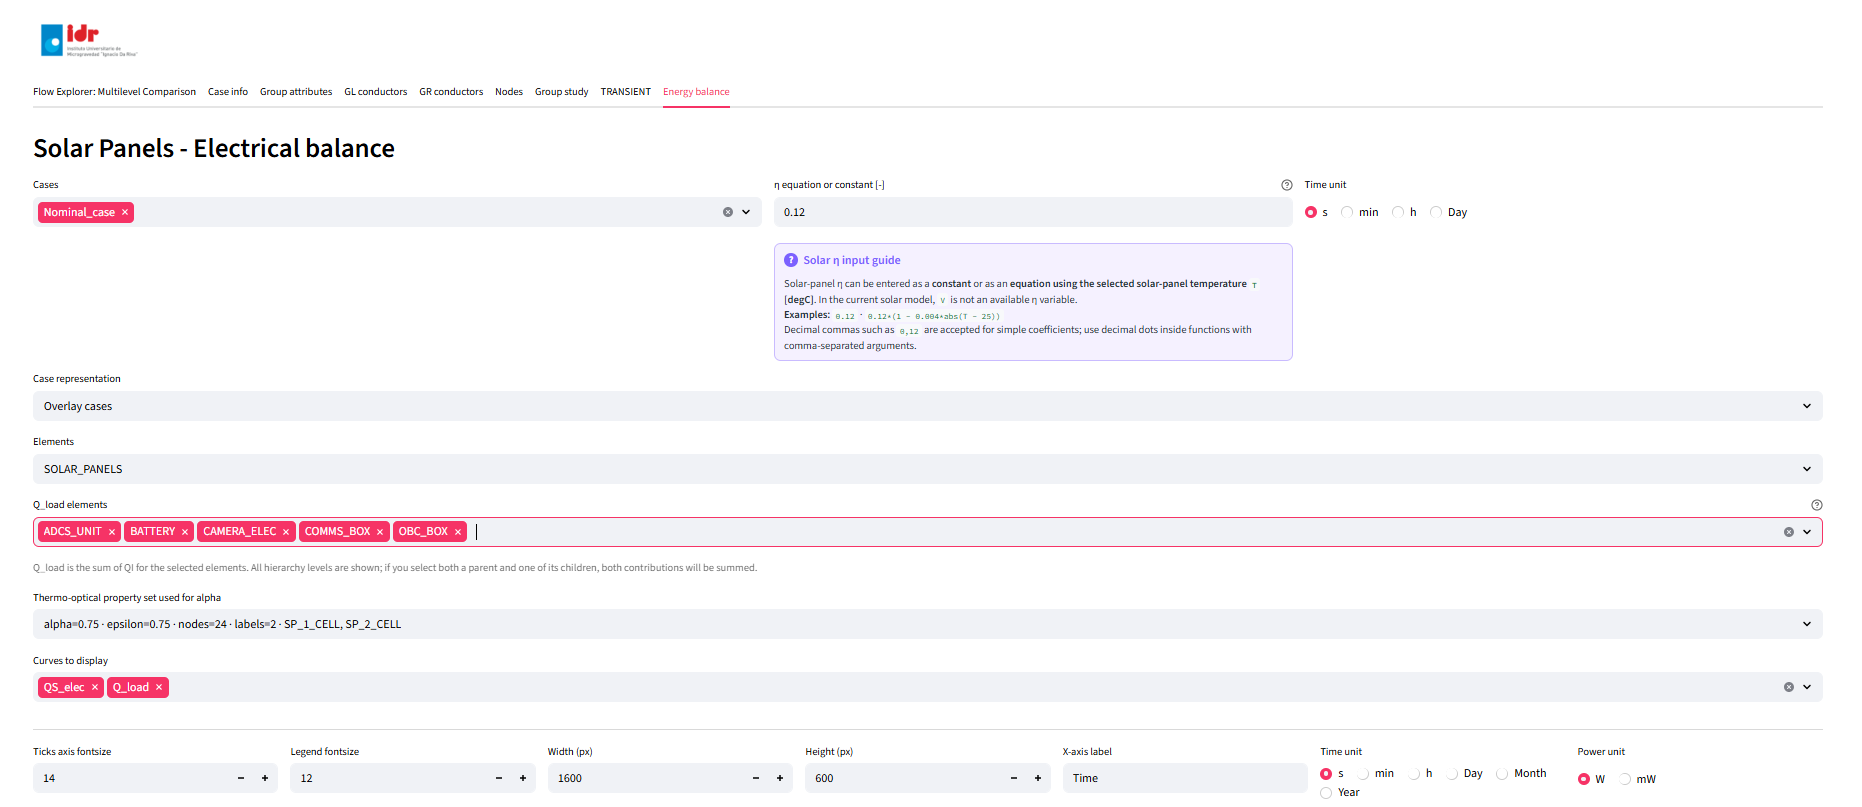
\includegraphics[
        width=0.98\textwidth,
        keepaspectratio
    ]{Figures/08/elec00.png}
    \caption{Configuration of the solar-to-electrical conversion and the
    electrical-load selection.}
    \label{fig:solar_electrical_configuration}
\end{figure}

The graph can display $Q_S$, $Q_{S,\mathrm{elec}}$ and
$Q_{\mathrm{load}}$ on the same time axis. The default selection compares the
available electrical generation with the estimated demand, which directly
reveals the charging and discharging intervals later used by the battery
model. Figure~\ref{fig:solar_electrical_balance_plot} illustrates this output.
Its numerical values only demonstrate the representation available in the tab;
the final case results belong to the subsequent results analysis.

\begin{figure}[H]
    \centering
    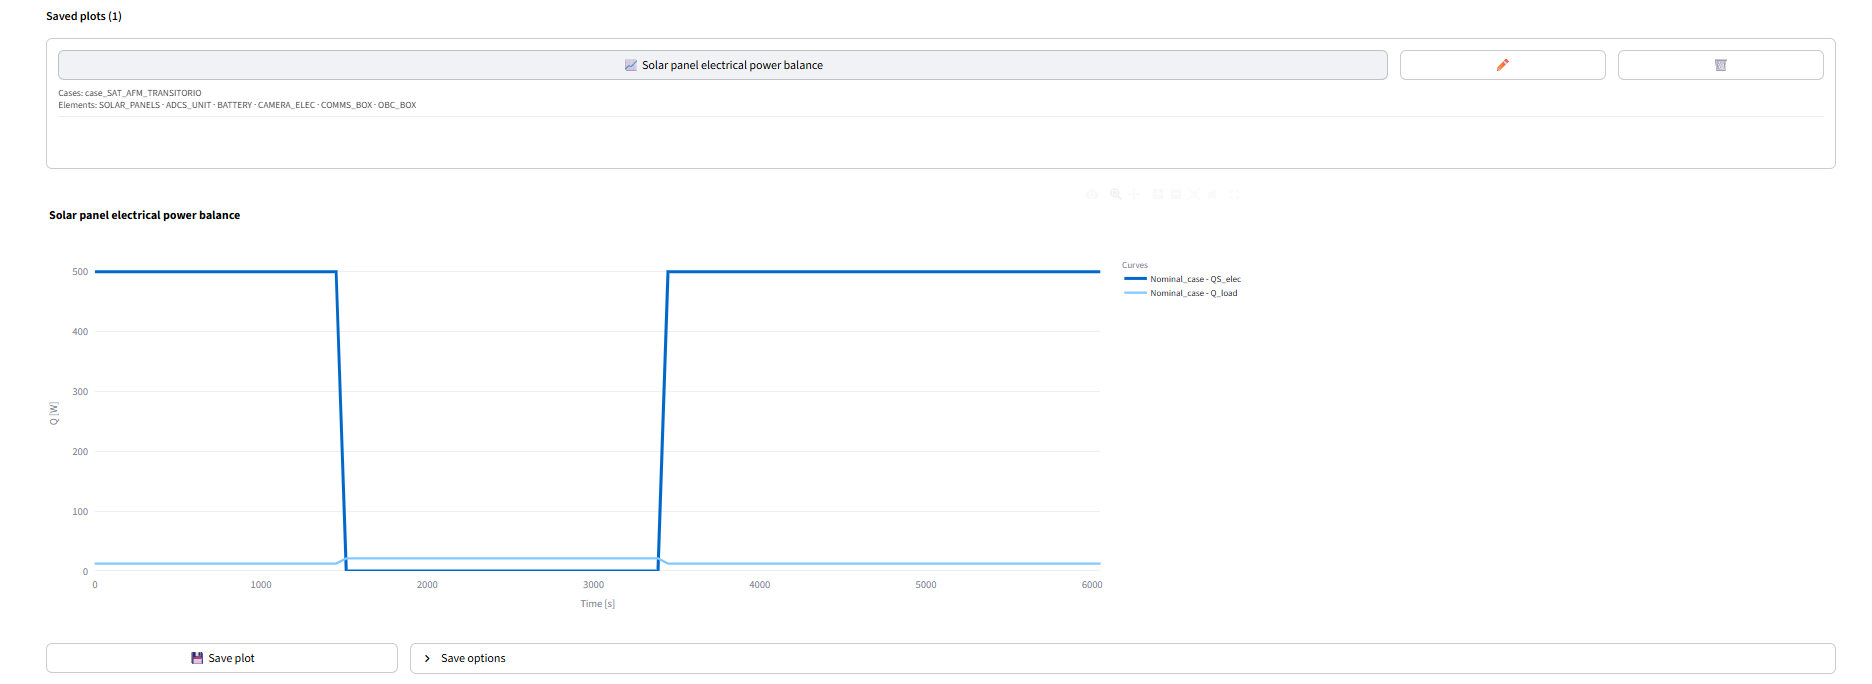
\includegraphics[
        width=0.97\textwidth,
        keepaspectratio
    ]{Figures/08/elec02.png}
    \caption{Illustrative solar-panel electrical balance containing
    $Q_{S,\mathrm{elec}}$ and $Q_{\mathrm{load}}$.}
    \label{fig:solar_electrical_balance_plot}
\end{figure}

An optional calculation table retains the values used at every output instant.
Its columns include $Q_S$, $Q_{S,i}$, $Q_{S,\mathrm{elec}}$,
$Q_{\mathrm{load}}$, $\alpha$, $\alpha_{\mathrm{th}}$ and $\eta$. When the
efficiency depends on temperature, the table also includes the temperature
history supplied to the efficiency expression. This output allows the user to
check the complete conversion before applying the result to the battery.


\section{Battery Model}
\label{sec:battery_model}

The battery calculation starts from the histories generated in the first part
of the tab. At each time interval, solar power first covers the selected load.
The model sends any remaining surplus to the battery and requests discharge
when generation cannot meet the demand. Battery temperature, conversion
efficiencies, voltage limits, internal resistance and charge-control settings
then determine the accepted power and the evolution of the stored energy.

The application recalculates the battery whenever the user changes the solar
element, the $Q_{\mathrm{load}}$ groups, the thermo-optical property, $\alpha$
or the solar-efficiency equation. Consequently, two identical battery
configurations can produce different responses when their upstream
$Q_{S,\mathrm{elec}}$ or $Q_{\mathrm{load}}$ histories differ.


\subsection{Energy-Discharge-Level Basis}
\label{subsec:battery_theoretical_basis}

The battery formulation takes the energy-discharge-level approach proposed by
Porras-Hermoso, Pindado and Cubas as its theoretical basis
\cite{porras2018battery}. Their equivalent-circuit model uses discharged
energy $\phi$ as the main state variable instead of relying only on discharged
ampere-hours. This choice relates the state directly to the exchanged power
and reduces the dependence of the capacity description on a single current
rate.

For a discharge process, the original formulation defines

\begin{equation}
    \phi(t)
    =
    \phi_0
    +
    \int_{t_0}^{t}
    \left[
        V I_d+R_d I_d^2
    \right]\mathrm{d}t,
    \label{eq:porras_discharge_energy_ch8}
\end{equation}

whereas charging decreases the discharged-energy level according to

\begin{equation}
    \phi(t)
    =
    \phi_0
    -
    \int_{t_0}^{t}
    \left[
        V I_c-R_c I_c^2
    \right]\mathrm{d}t.
    \label{eq:porras_charge_energy_ch8}
\end{equation}

Here, $I_d$ and $I_c$ denote the non-negative discharge and charge current
magnitudes, while $R_d$ and $R_c$ represent the corresponding internal
resistances. The terminal voltage follows

\begin{align}
    V_d(\phi,I_d)
    &=
    E_d(\phi)-R_d I_d,
    \label{eq:porras_discharge_voltage_ch8}
    \\
    V_c(\phi,I_c)
    &=
    E_c(\phi)+R_c I_c.
    \label{eq:porras_charge_voltage_ch8}
\end{align}

Porras-Hermoso et al. identify $E_d(\phi)$ and $E_c(\phi)$ from experimental
charge and discharge curves and extend the static equivalent circuit with
additional resistor--capacitor branches for dynamic operation
\cite{porras2018battery}.

The implementation developed for this project retains the energy state, the
separate charge and discharge resistances, and the terminal-voltage relations.
It does not reproduce the experimentally fitted voltage functions or the
dynamic resistor--capacitor branches. Instead, it constructs a generic
piecewise-linear internal-voltage curve $E(\phi)$ from the cell discharge
cut-off, nominal and charge-limit voltages. This reduction keeps the model
configurable when no calibration data exist for a particular flight battery.

Let $C_{\mathrm{pack,Wh}}$ denote the nominal energy capacity and
$E_{\mathrm{st}}(t)$ the stored energy. The implemented discharged-energy
state becomes

\begin{equation}
    \phi(t)
    =
    C_{\mathrm{pack,Wh}}-E_{\mathrm{st}}(t),
    \label{eq:implemented_battery_phi}
\end{equation}

and the reported state of charge follows

\begin{equation}
    \mathrm{SOC}(t)
    =
    100
    \frac{E_{\mathrm{st}}(t)}{C_{\mathrm{pack,Wh}}}.
    \label{eq:implemented_battery_soc}
\end{equation}

The module solves the corresponding relation $P=VI$ to obtain current from the
power requested at each step. It also adds conversion efficiencies, charge and
discharge power limits, temperature-dependent charge derating and a simplified
CC--CV strategy. The resulting curves provide engineering estimates for the
selected configuration rather than an experimentally calibrated prediction of
a specific battery.


\subsection{Thermal Derating and Battery-Pack Configuration}
\label{subsec:battery_configuration}

The first parameter block links the battery calculation with the thermal
solution and defines the physical pack. The \emph{Battery TMD element}
selector identifies the group whose mean temperature represents the battery.
The model uses this history in the charge-derating calculation and in any
charge or discharge efficiency expression that contains $T$.

The lower and upper derating limits define the temperature interval in which
the battery accepts charge. A common ramp margin $m_T$ softens both
transitions. For non-overlapping lower and upper ramps, the implemented factor
can be written as

\begin{equation}
    f_T(T)
    =
    \begin{cases}
        0,
        & T\leq T_{\mathrm{low}},
        \\[0.35em]
        \dfrac{T-T_{\mathrm{low}}}{m_T},
        & T_{\mathrm{low}}<T<T_{\mathrm{low}}+m_T,
        \\[0.9em]
        1,
        & T_{\mathrm{low}}+m_T
          \leq T\leq
          T_{\mathrm{high}}-m_T,
        \\[0.35em]
        \dfrac{T_{\mathrm{high}}-T}{m_T},
        & T_{\mathrm{high}}-m_T<T<T_{\mathrm{high}},
        \\[0.9em]
        0,
        & T\geq T_{\mathrm{high}}.
    \end{cases}
    \label{eq:battery_charge_derating_ch8}
\end{equation}

The factor multiplies the maximum charge current and charge power. A value of
one allows normal charging, a value of zero blocks it, and intermediate values
reduce the accepted surplus linearly. The derating does not limit discharge in
the current implementation.

The cell configuration uses $N_s$ cells in series and $N_p$ parallel strings.
The application obtains the equivalent pack voltages from

\begin{equation}
    V_{x,\mathrm{pack}}
    =
    N_sV_{x,\mathrm{cell}},
    \qquad
    x\in\{\mathrm{cut},\mathrm{nom},\mathrm{chg}\},
    \label{eq:battery_pack_voltages}
\end{equation}

while the charge and nominal energy capacities become

\begin{align}
    C_{\mathrm{pack,Ah}}
    &=
    N_p C_{\mathrm{cell,Ah}},
    \label{eq:battery_pack_ah}
    \\
    C_{\mathrm{pack,Wh}}
    &=
    V_{\mathrm{nom,pack}}C_{\mathrm{pack,Ah}}.
    \label{eq:battery_pack_wh}
\end{align}

The initial SOC fixes the energy available at the first output instant:

\begin{equation}
    E_{\mathrm{st},0}
    =
    \frac{\mathrm{SOC}_0}{100}C_{\mathrm{pack,Wh}}.
    \label{eq:battery_initial_energy}
\end{equation}

Table~\ref{tab:battery_thermal_pack_inputs} summarises every field in this
first parameter block.

\begin{table}[H]
    \centering
    \caption{Battery thermal and pack-configuration inputs.}
    \label{tab:battery_thermal_pack_inputs}
    \small
    \setlength{\tabcolsep}{4pt}
    \renewcommand{\arraystretch}{1.15}
    \begin{tabularx}{\textwidth}{@{}p{0.35\textwidth}X@{}}
        \toprule
        \textbf{Interface field} & \textbf{Role in the calculation} \\
        \midrule

        Battery TMD element &
        Supplies the mean battery temperature used by charge derating and
        temperature-dependent efficiency expressions. \\

        Charge derating lower limit &
        Blocks charging below the selected lower temperature. \\

        Charge derating upper limit &
        Blocks charging above the selected upper temperature. \\

        Charge derating ramp margin &
        Defines the linear transition band beside both charging limits. \\

        Series cells $N_s$ &
        Scales the pack cut-off, nominal and charge-limit voltages. \\

        Parallel strings $N_p$ &
        Scales pack charge capacity and reduces equivalent resistance. \\

        Cell charge capacity &
        Defines the ampere-hour capacity of one cell and, together with $N_p$,
        the pack charge capacity. \\

        Cell discharge cut-off voltage &
        Defines the minimum admissible cell voltage during discharge. \\

        Cell nominal/reference voltage &
        Defines the nominal pack voltage and the conversion from Ah to Wh. \\

        Cell charge voltage limit &
        Defines the upper terminal-voltage limit used during charging. \\

        Initial SOC &
        Sets the stored energy at the start of the transient calculation. \\

        \bottomrule
    \end{tabularx}
\end{table}

Figure~\ref{fig:battery_thermal_pack_configuration} shows the corresponding
controls in the application.

\begin{figure}[H]
    \centering
    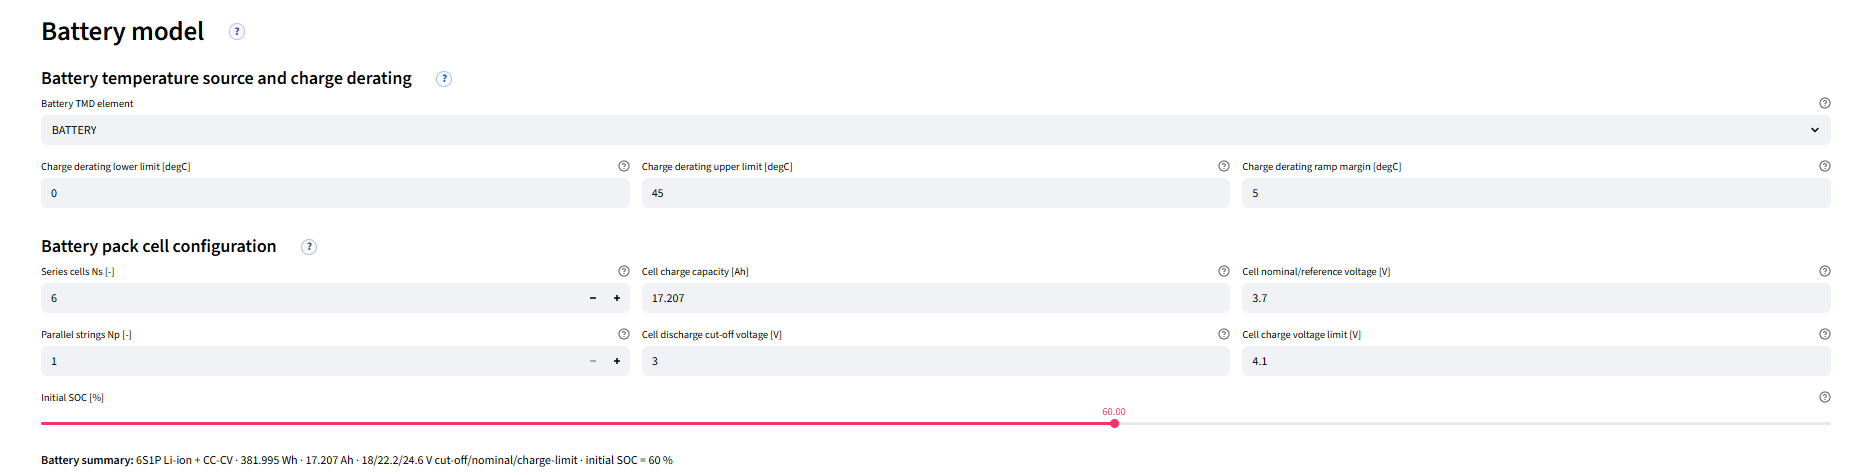
\includegraphics[
        width=0.98\textwidth,
        keepaspectratio
    ]{Figures/08/bat00.png}
    \caption{Battery-temperature reference, charge derating and cell-pack
    configuration.}
    \label{fig:battery_thermal_pack_configuration}
\end{figure}


\subsection{Electrical Parameters and CC--CV Charge Control}
\label{subsec:battery_electrical_parameters}

The second parameter block defines the power-transfer behaviour of the pack.
Charge and discharge efficiencies may use constants or expressions of battery
temperature $T$ and terminal voltage $V$:

\begin{equation}
    \eta_c(t)=f_c\!\left[T_{\mathrm{batt}}(t),V(t)\right],
    \qquad
    \eta_d(t)=f_d\!\left[T_{\mathrm{batt}}(t),V(t)\right].
    \label{eq:battery_efficiency_functions}
\end{equation}

The application requires $0<\eta_c\leq1$ and $0<\eta_d\leq1$. Constants form
the simplest valid expressions. During charge, $\eta_c$ reduces the solar
surplus that reaches the battery terminals. During discharge, $\eta_d$ reduces
the terminal power delivered to the electrical load. The model reports the
remaining difference as conversion loss.

Separate cell resistances retain the charge--discharge asymmetry of the
energy-based equivalent circuit. Their pack values follow

\begin{equation}
    R_{x,\mathrm{pack}}
    =
    R_{x,\mathrm{cell}}
    \frac{N_s}{N_p},
    \qquad
    x\in\{d,c\}.
    \label{eq:battery_pack_resistance_ch8}
\end{equation}

The resistance lowers the discharge terminal voltage and raises the charge
terminal voltage. It also produces the internal loss

\begin{equation}
    P_{\mathrm{loss,int}}(t)
    =
    R I^2(t).
    \label{eq:battery_internal_loss_ch8}
\end{equation}

Maximum charge and discharge powers establish independent caps for both
operating directions. During charging, the CC current ceiling follows the
selected C-rate:

\begin{equation}
    I_{\mathrm{CC,max}}
    =
    C_{\mathrm{rate}}C_{\mathrm{pack,Ah}}.
    \label{eq:battery_cc_current_ch8}
\end{equation}

The temperature factor from Equation~\eqref{eq:battery_charge_derating_ch8}
reduces this ceiling and the maximum charge power. The voltage constraint also
requires

\begin{equation}
    E(\phi)+R_cI_c
    \leq
    V_{\mathrm{chg,pack}}.
    \label{eq:battery_cv_voltage_limit}
\end{equation}

Above the selected SOC threshold $\mathrm{SOC}_{\mathrm{CV}}$, an additional
factor progressively reduces the current:

\begin{equation}
    f_{\mathrm{CV}}(\mathrm{SOC})
    =
    \left[
        \frac{100-\mathrm{SOC}}
        {100-\mathrm{SOC}_{\mathrm{CV}}}
    \right]^{\gamma},
    \qquad
    \mathrm{SOC}\geq\mathrm{SOC}_{\mathrm{CV}},
    \label{eq:battery_cv_taper_ch8}
\end{equation}

where $\gamma$ controls the shape of the reduction. The current remains
subject to the CC limit below this threshold, provided that the solar surplus
and charge-power cap allow it. The model declares practical full charge when
the tapered or voltage-limited current falls below the selected current
threshold; any additional surplus then appears as curtailed solar power.

During discharge, the model limits current through the available stored
energy, the maximum discharge power and the cell discharge cut-off voltage.
Any demand that remains after these restrictions appears as unserved load.

Table~\ref{tab:battery_electrical_inputs} collects every field in this second
parameter block.

\begin{table}[H]
    \centering
    \caption{Battery electrical and CC--CV control inputs.}
    \label{tab:battery_electrical_inputs}
    \small
    \setlength{\tabcolsep}{4pt}
    \renewcommand{\arraystretch}{1.15}
    \begin{tabularx}{\textwidth}{@{}p{0.39\textwidth}X@{}}
        \toprule
        \textbf{Interface field} & \textbf{Role in the calculation} \\
        \midrule

        Charge efficiency equation &
        Defines the fraction of solar surplus transferred towards battery
        charging; it may depend on $T$ and $V$. \\

        Discharge efficiency equation &
        Defines the fraction of terminal discharge power delivered to the
        selected electrical load; it may depend on $T$ and $V$. \\

        Maximum charge power &
        Caps the terminal power accepted from the solar surplus. \\

        Maximum discharge power &
        Caps the terminal power extracted when generation does not cover the
        demand. \\

        Maximum constant-current charge rate &
        Sets the CC current ceiling as a multiple of pack capacity in Ah. \\

        SOC where current reduction towards CV begins &
        Defines the SOC threshold above which the taper factor acts. \\

        Current-reduction shape factor &
        Controls how sharply charge current decreases near full charge. \\

        Charge-complete current threshold &
        Stops charging when the reduced current falls below the selected
        practical limit in the CV region. \\

        Cell discharge internal resistance &
        Determines pack voltage drop and $I^2R$ loss during discharge. \\

        Cell charge internal resistance &
        Determines pack voltage rise and $I^2R$ loss during charge. \\

        \bottomrule
    \end{tabularx}
\end{table}

Figure~\ref{fig:battery_electrical_configuration} shows these controls. The
summary box below the inputs reports the resulting voltage limits, equivalent
pack resistances and an efficiency preview for the current configuration.

\begin{figure}[H]
    \centering
    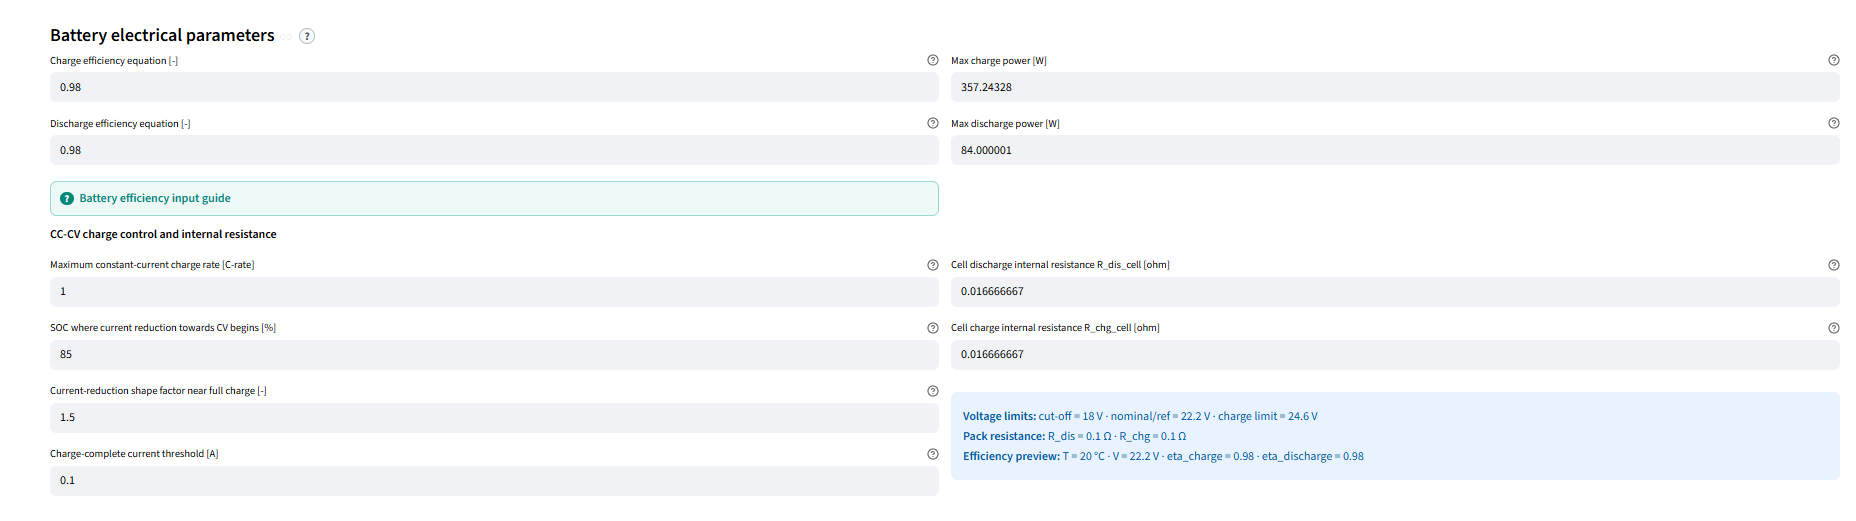
\includegraphics[
        width=0.98\textwidth,
        keepaspectratio
    ]{Figures/08/bat01.png}
    \caption{Battery efficiencies, power limits, internal resistances and
    simplified CC--CV control parameters.}
    \label{fig:battery_electrical_configuration}
\end{figure}


\subsection{Battery Output Curves and Summary Results}
\label{subsec:battery_outputs}

The tab places the graphical outputs immediately after the parameter blocks so
that the user can inspect the effect of each change without leaving the
battery workflow. The first graph shows state of charge throughout the
simulation. Rising segments indicate net storage, falling segments indicate
battery support of the load, and horizontal segments identify intervals in
which the stored energy remains unchanged or reaches an operating limit.

\begin{figure}[H]
    \centering
    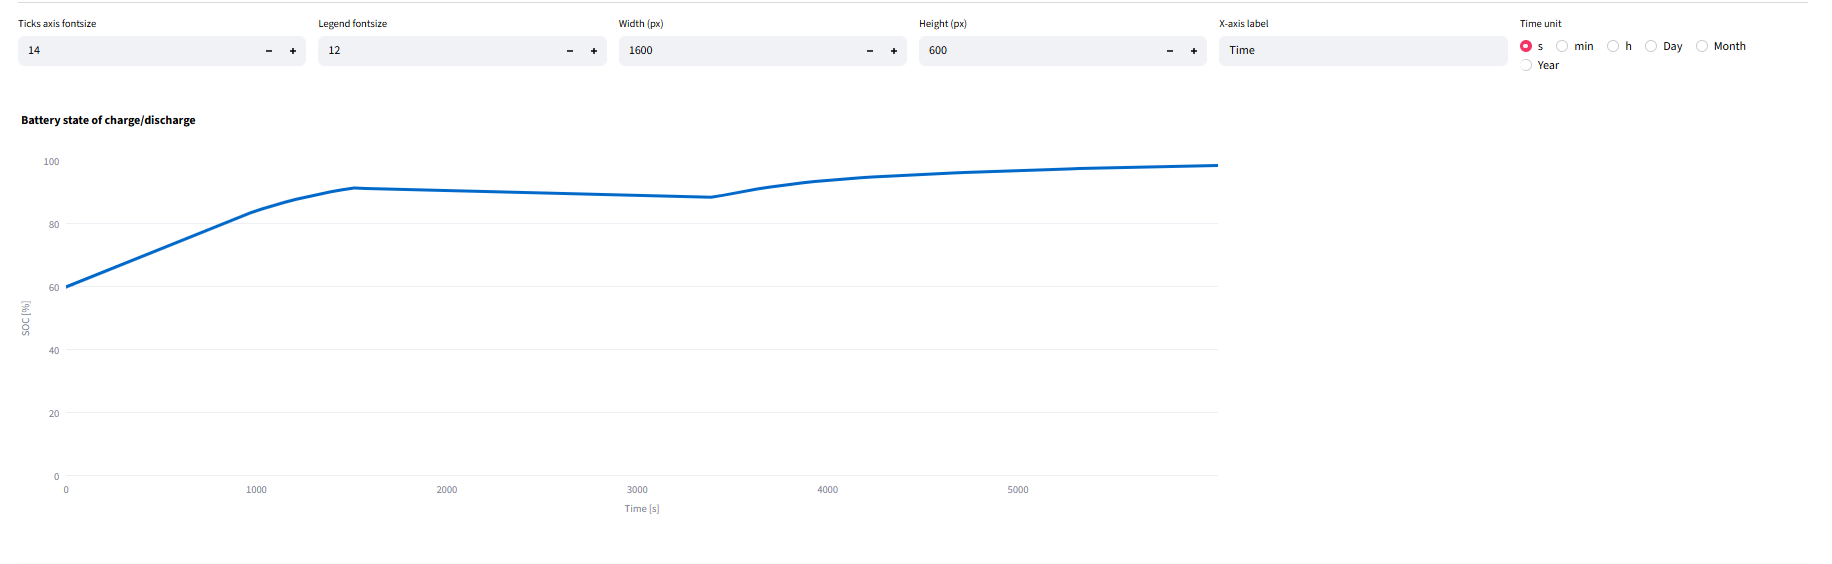
\includegraphics[
        width=0.97\textwidth,
        keepaspectratio
    ]{Figures/08/bat02.png}
    \caption{Illustrative battery state-of-charge history.}
    \label{fig:battery_soc_output}
\end{figure}

The second graph combines terminal voltage with separate non-negative charge
and discharge currents. The left axis represents voltage, while the right axis
represents current. The separation of both current directions avoids relying
on a sign convention in the graphical interpretation, although the detailed
calculation table also retains a signed battery current that is positive in
discharge and negative in charge.

\begin{figure}[H]
    \centering
    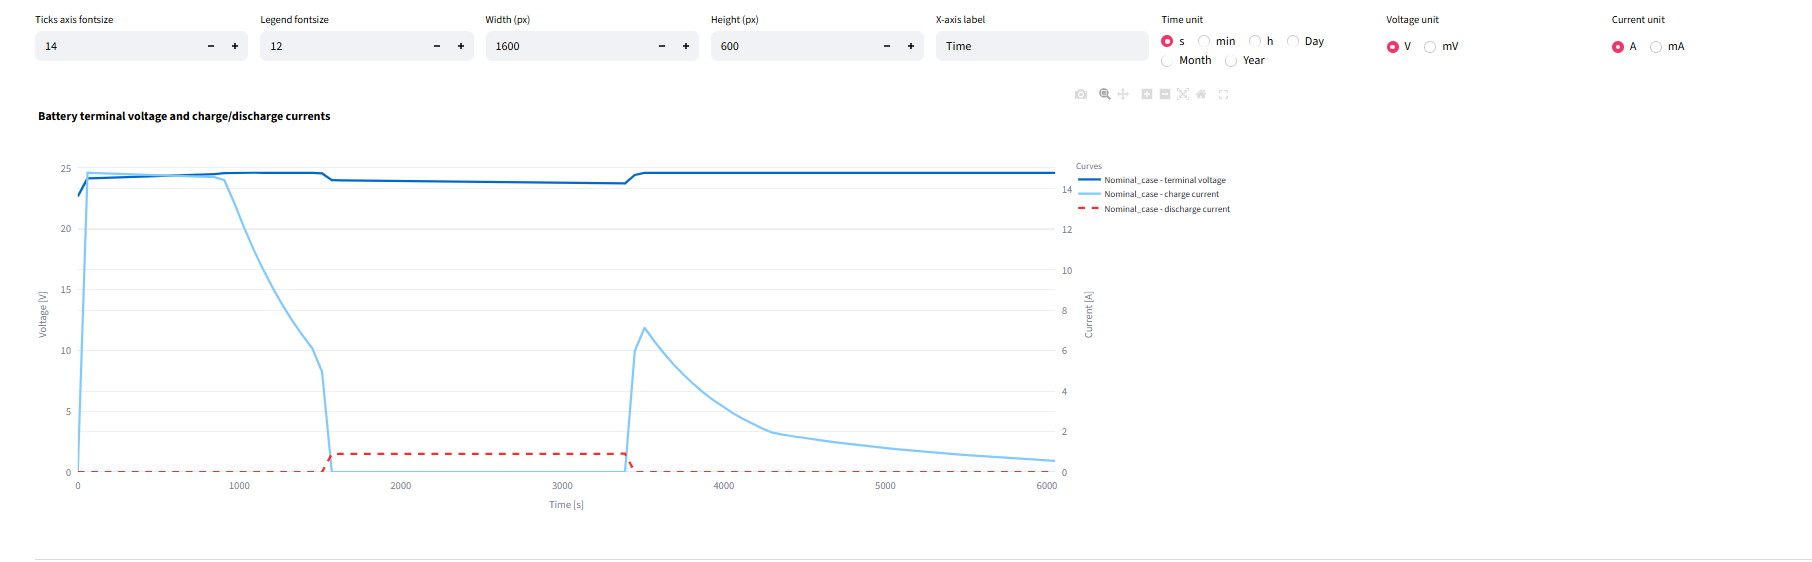
\includegraphics[
        width=0.97\textwidth,
        keepaspectratio
    ]{Figures/08/bat03.png}
    \caption{Illustrative terminal-voltage and charge/discharge-current
    histories.}
    \label{fig:battery_voltage_current_output}
\end{figure}

The third graph connects the thermal result with the battery restrictions. It
places the mean battery temperature on the left axis and the charge-derating,
charge-efficiency and discharge-efficiency factors on the right. This output
shows whether a change in battery behaviour comes from the available power,
the selected efficiency expressions or a temperature-dependent charging
restriction.

\begin{figure}[H]
    \centering
    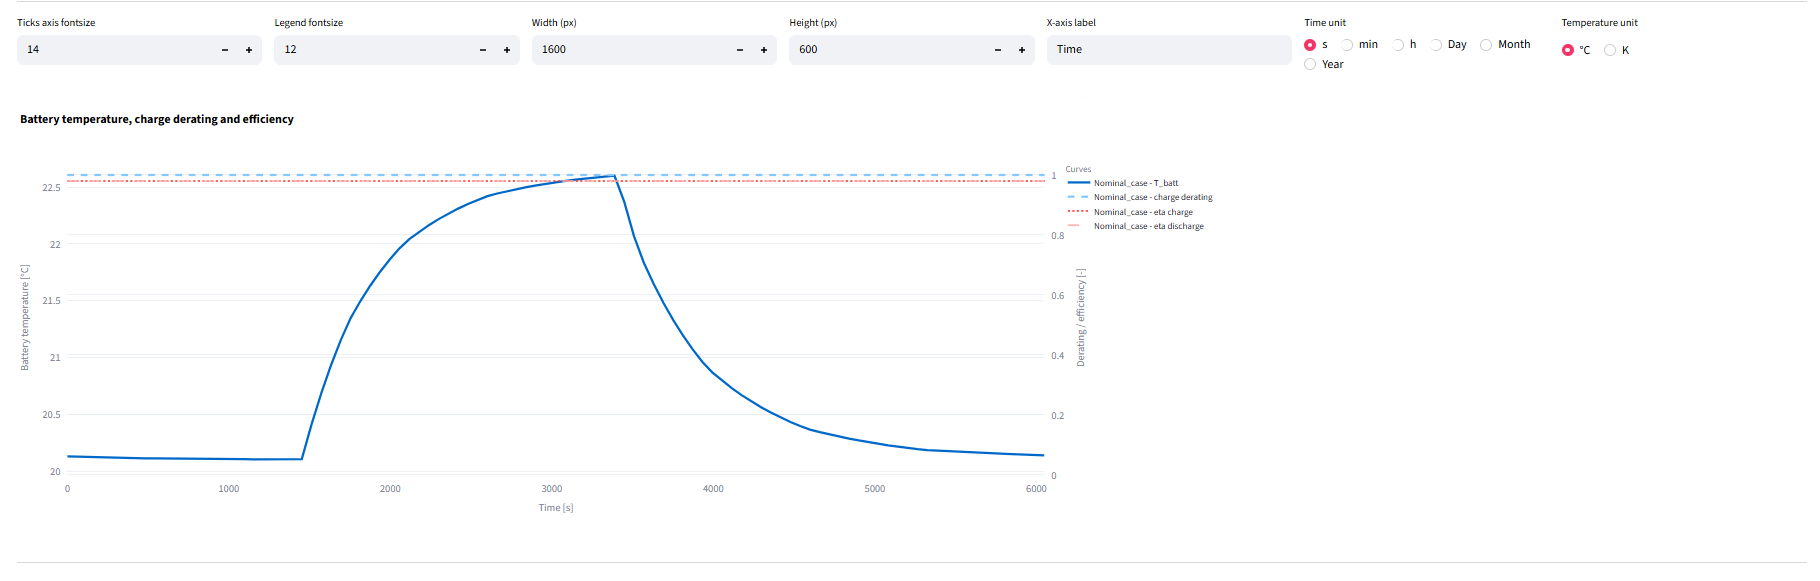
\includegraphics[
        width=0.97\textwidth,
        keepaspectratio
    ]{Figures/08/bat_04.png}
    \caption{Illustrative battery temperature, charge-derating and efficiency
    histories.}
    \label{fig:battery_thermal_output}
\end{figure}

The figures in this subsection demonstrate the form of the available outputs;
they do not yet support conclusions about the final nominal, hot or cold
cases. Their numerical interpretation requires the validated input parameters
and belongs to the results stage of the project.

After the graphs, the battery summary table condenses the complete simulation.
It reports final, minimum and maximum SOC; maximum charge and discharge power;
curtailed solar energy; unserved-load energy; time spent in CC, CV,
solar-limited charge, discharge and voltage-limited discharge; minimum and
maximum battery temperature; minimum derating factor; total derated time; and
the ranges of charge and discharge efficiency.

A second, optional calculation table retains the values at every output
instant. Its principal columns include
$Q_{S,\mathrm{elec}}$, $Q_{\mathrm{load}}$, direct solar supply, surplus,
deficit, charge and discharge powers, terminal and internal voltages, charge
and discharge currents, SOC, $\phi$, stored energy, efficiencies, curtailed
solar power, unserved load, internal and conversion losses, battery
temperature, derating factor and operating phase. Together, the graphs and
tables connect the selected thermal case with the complete electrical and
battery post-processing sequence.

\cleardoublepage

\chapter[Multi-Case Results and Discussion]
{Multi-Case Results\\and Discussion}
\label{ch:results_discussion}

The nominal, hot and cold transient solutions are compared using the common
thermal model defined in Chapter~\ref{ch:thermal_model}. Geometry, nodal
hierarchy, materials and thermal couplings remain unchanged, while the
radiative environment and internal dissipations vary between cases. The
common output-time vector permits a direct comparison throughout the complete
simulated interval.

Absolute curves preserve the temperature, power, heat-flow and energy levels
of each solution. The \textit{Case difference} representation is added when a
direct subtraction provides a clearer measure of the separation from the
nominal case. The electrical conversion and battery model retain the inputs
defined in Chapter~\ref{ch:electrical_battery_analysis}; consequently, their
variations originate from the imported thermal results and the case-dependent
load profiles.


\section{Cases and Comparison Criteria}
\label{sec:comparison_criteria}

The three simulations correspond to the cases listed in
Table~\ref{tab:transient_cases}. The hot case combines greater external heat
input, higher internal dissipations and a shorter eclipse. The cold case
applies lower external input, reduced dissipations and a longer eclipse. No
heater operation is included. The same groups, attributes, source--target
ordering and units are retained whenever the cases are superposed.

For a result $x(t)$, the difference between the nominal case $N$ and a
comparison case $j$ is defined as
\begin{equation}
    \Delta x_{N-j}(t)
    =
    x_N(t)-x_j(t),
    \qquad
    j\in\{H,C\},
    \label{eq:results_case_difference}
\end{equation}
where $H$ and $C$ denote the hot and cold cases. A negative value of
$\Delta x_{N-H}$ therefore indicates that the hot-case result exceeds the
nominal value. This convention is retained in every plot and table generated
with \textit{Case difference}. Absolute curves are preferred when the
operating level is relevant, whereas differences are used to quantify the
separation between solutions or to expose changes hidden by overlapping
curves.


\section{Thermal Response}
\label{sec:thermal_results_comparison}

Applied loads establish the heating and cooling intervals, while the resulting
temperatures determine spatial differences, interface gradients and heat
exchanges.


\subsection{Applied Loads and Temperatures}
\label{subsec:loads_temperature_comparison}

Figure~\ref{fig:solar_panel_load_temperature_comparison} combines the
direct-solar load and mean temperature of \texttt{SOLAR\_PANEL\_1}. The hot
case receives the largest solar input and remains illuminated until the late
part of the simulation. Its eclipse covers only approximately the interval
from $84$ to $96\,\mathrm{min}$. The nominal eclipse extends from about $25$
to $56\,\mathrm{min}$, while the cold case remains without direct solar input
from approximately $42$ to $77\,\mathrm{min}$.

\begin{figure}[H]
    \centering
    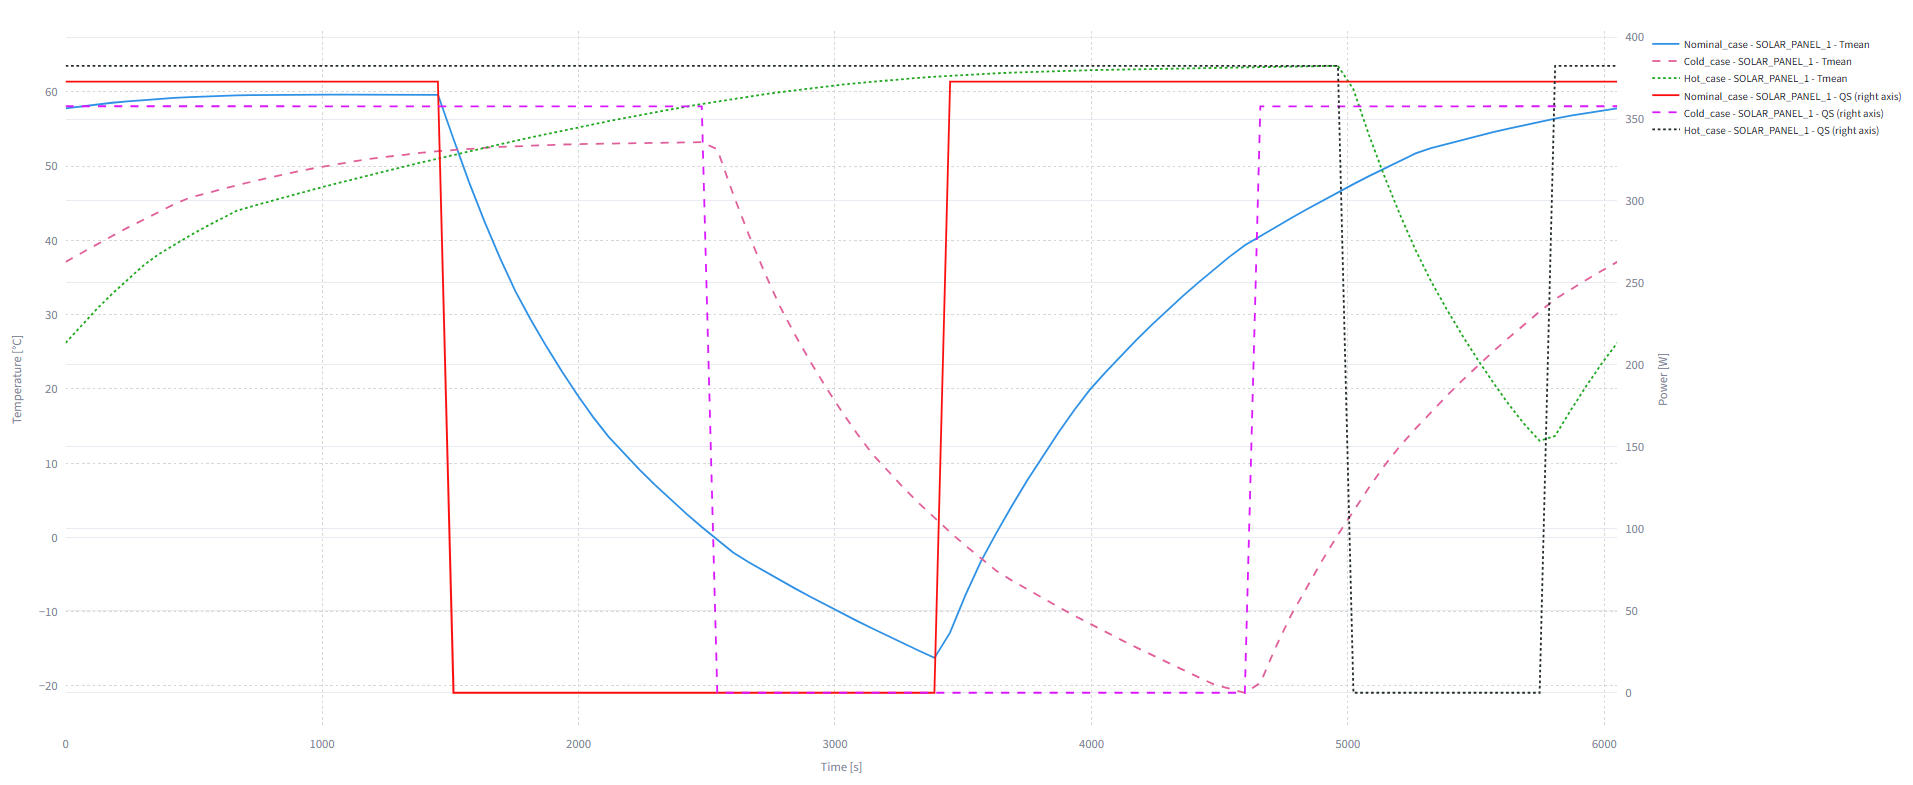
\includegraphics[
        width=1.0\textwidth,
        keepaspectratio
    ]{Figures/09/solar_panel_load_temperature_comparison.png}
    \caption{Direct-solar thermal load and mean temperature of
    \texttt{SOLAR\_PANEL\_1} in the nominal, hot and cold cases.}
    \label{fig:solar_panel_load_temperature_comparison}
\end{figure}

The panel temperature follows the illumination sequence with a delayed
response during each transition. The hot case reaches the highest nodal
temperature, $65.42\,^{\circ}\mathrm{C}$, and remains above
$12.15\,^{\circ}\mathrm{C}$ because of its short eclipse. The nominal and
cold cases cool to $-17.25\,^{\circ}\mathrm{C}$ and
$-21.31\,^{\circ}\mathrm{C}$, respectively. The maximum spatial range inside
\texttt{SOLAR\_PANEL\_1} increases from $5.78\,^{\circ}\mathrm{C}$ in the
hot case to $8.52\,^{\circ}\mathrm{C}$ in the nominal case and
$10.14\,^{\circ}\mathrm{C}$ in the cold case. The lower overall temperature
of the cold solution is therefore accompanied by the largest internal
non-uniformity of the selected panel group.

The internal battery dissipation and mean temperature are compared in
Figure~\ref{fig:battery_load_temperature_comparison}. The prescribed load is
largest in the hot case and smallest in the cold case, both inside and outside
eclipse. The temperature response preserves the same ordering throughout the
simulation: the hot battery remains near $36$--$38\,^{\circ}\mathrm{C}$, the
nominal battery near $18$--$21\,^{\circ}\mathrm{C}$ and the cold battery near
$4\,^{\circ}\mathrm{C}$.

\begin{figure}[H]
    \centering
    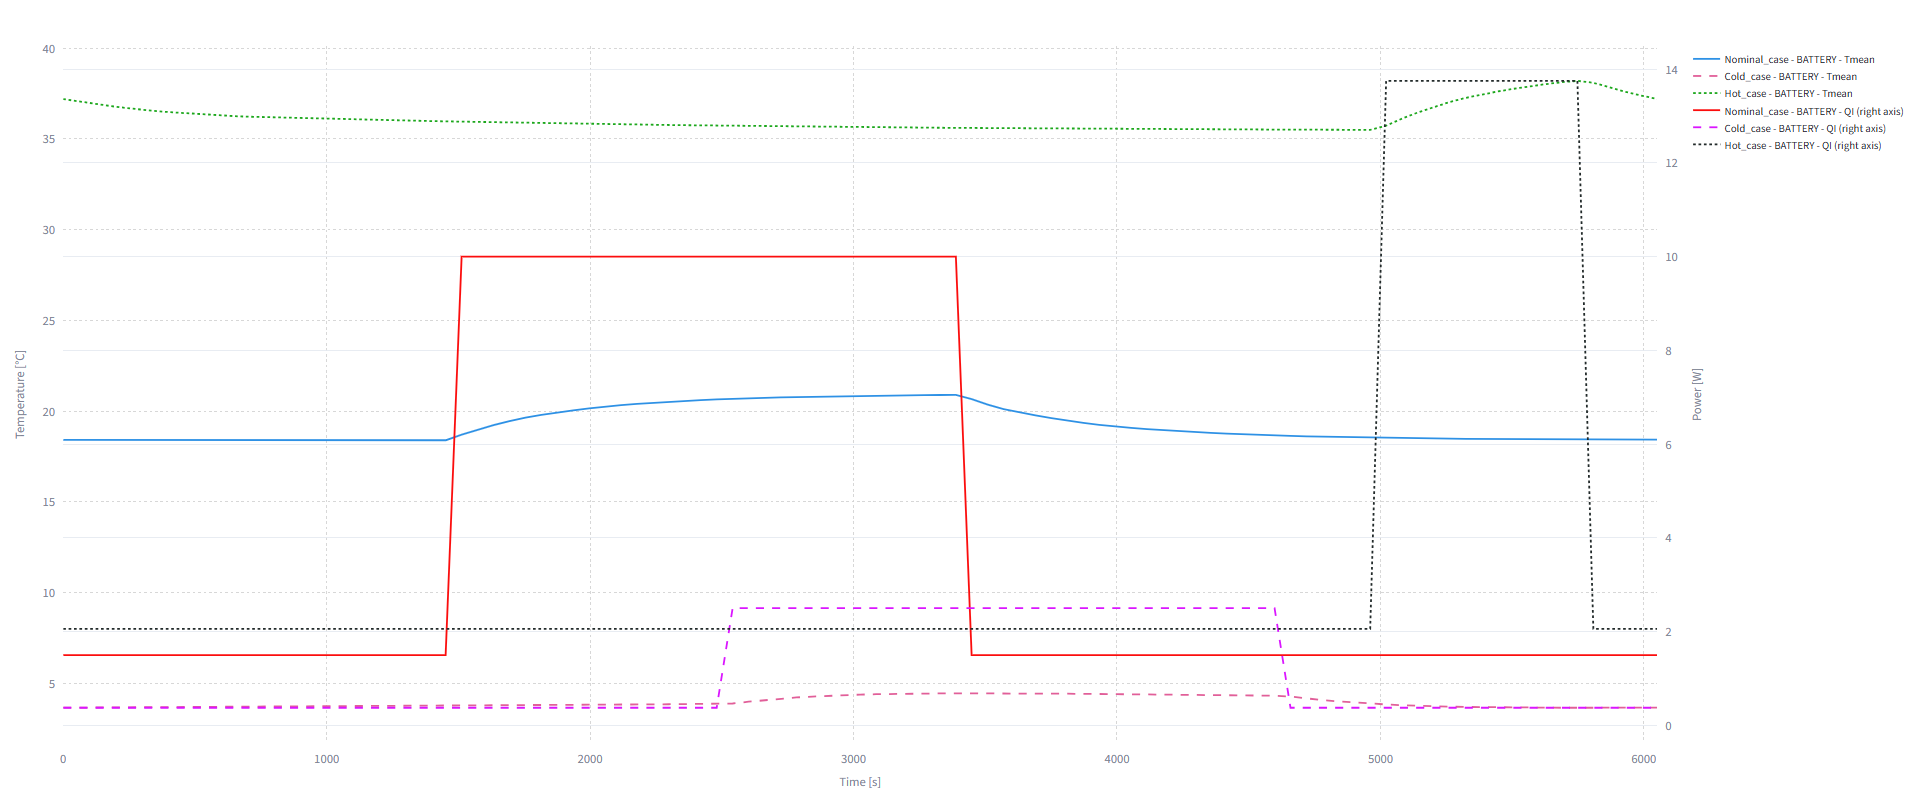
\includegraphics[
        width=0.9\textwidth,
        keepaspectratio
    ]{Figures/09/battery_load_temperature_comparison.png}
    \caption{Internal heat load and mean temperature of \texttt{BATTERY} in
    the three transient cases.}
    \label{fig:battery_load_temperature_comparison}
\end{figure}

The nodal extrema in Table~\ref{tab:multicase_thermal_summary} confirm the
general displacement of the thermal response. The hot case produces the
highest temperatures for all selected elements, whereas the cold case
produces the lowest. The shift is particularly clear in the battery, OBC and
radiator. Battery temperatures range from $35.43$ to
$38.97\,^{\circ}\mathrm{C}$ in the hot case, from $18.25$ to
$21.77\,^{\circ}\mathrm{C}$ in the nominal case and from $3.50$ to
$4.60\,^{\circ}\mathrm{C}$ in the cold case. The radiator follows the same
trend but remains substantially colder, reaching minima of
$5.56\,^{\circ}\mathrm{C}$, $-7.37\,^{\circ}\mathrm{C}$ and
$-17.26\,^{\circ}\mathrm{C}$, respectively.

% File: Tables/table_multicase_thermal_summary.tex
% Usage: \MultiCaseThermalSummaryTable[0.82\textwidth]
% Values obtained from the thermal-summary exports for the nominal, hot and
% cold transient cases.

\newcommand{\MultiCaseThermalSummaryTable}[1][0.82\textwidth]{%
\begin{table}[H]
    \centering
    \caption{Temperature extrema and maximum spatial temperature ranges of
    the selected elements in the nominal, hot and cold transient cases.}
    \label{tab:multicase_thermal_summary}
    \footnotesize
    \renewcommand{\arraystretch}{1.16}
    \setlength{\tabcolsep}{5.0pt}
    \resizebox{#1}{!}{%
    \begin{tabular}{|l|l|c|c|c|}
        \hline
        \textbf{Element} &
        \textbf{Case} &
        \textbf{$T_{\max}$ [$^\circ$C]} &
        \textbf{$T_{\min}$ [$^\circ$C]} &
        \textbf{$\Delta T_{\max}^{\mathrm{sp}}$ [$^\circ$C]} \\ \hline

        \texttt{SOLAR\_PANEL\_1} & Nominal & 62.45 & -17.25 & 8.52 \\ \cline{2-5}
        & Hot  & 65.42 & 12.15  & 5.78 \\ \cline{2-5}
        & Cold & 56.63 & -21.31 & 10.14 \\ \hline

        \texttt{BODY\_PANEL} & Nominal & 18.87 & 5.05  & 13.63 \\ \cline{2-5}
        & Hot  & 35.76 & 20.90 & 14.72 \\ \cline{2-5}
        & Cold & 5.63  & -5.55 & 10.99 \\ \hline

        \texttt{OBC\_BOX} & Nominal & 13.74 & 11.30 & 2.36 \\ \cline{2-5}
        & Hot  & 30.43 & 27.83 & 2.59 \\ \cline{2-5}
        & Cold & 0.85  & -1.28 & 2.05 \\ \hline

        \texttt{RADIATOR} & Nominal & 0.05   & -7.37  & 5.66 \\ \cline{2-5}
        & Hot  & 14.49  & 5.56   & 6.68 \\ \cline{2-5}
        & Cold & -10.85 & -17.26 & 4.88 \\ \hline

        \texttt{BATTERY} & Nominal & 21.77 & 18.25 & 2.98 \\ \cline{2-5}
        & Hot  & 38.97 & 35.43 & 2.90 \\ \cline{2-5}
        & Cold & 4.60  & 3.50  & 0.84 \\ \hline
    \end{tabular}%
    }
\end{table}%
}

\MultiCaseThermalSummaryTable[0.62\textwidth]

The absolute temperature levels do not determine the spatial ranges by
themselves. The hot \texttt{BODY\_PANEL} reaches the largest internal range,
$14.72\,^{\circ}\mathrm{C}$, but the cold battery presents the smallest
battery range, only $0.84\,^{\circ}\mathrm{C}$. The common network therefore
transfers the environmental shift differently according to the geometry,
connections and local dissipations of each group.

The separation of the mean battery temperatures is isolated in
Figure~\ref{fig:battery_temperature_difference}. The nominal-minus-cold curve
remains positive, between approximately $14$ and $17\,^{\circ}\mathrm{C}$,
whereas the nominal-minus-hot curve remains negative and reaches
$-19.75\,^{\circ}\mathrm{C}$ at $95.80\,\mathrm{min}$. The signs agree with
the reference-minus-comparison convention and make the thermal displacement
more visible than the superposed absolute curves.

\begin{figure}[H]
    \centering
    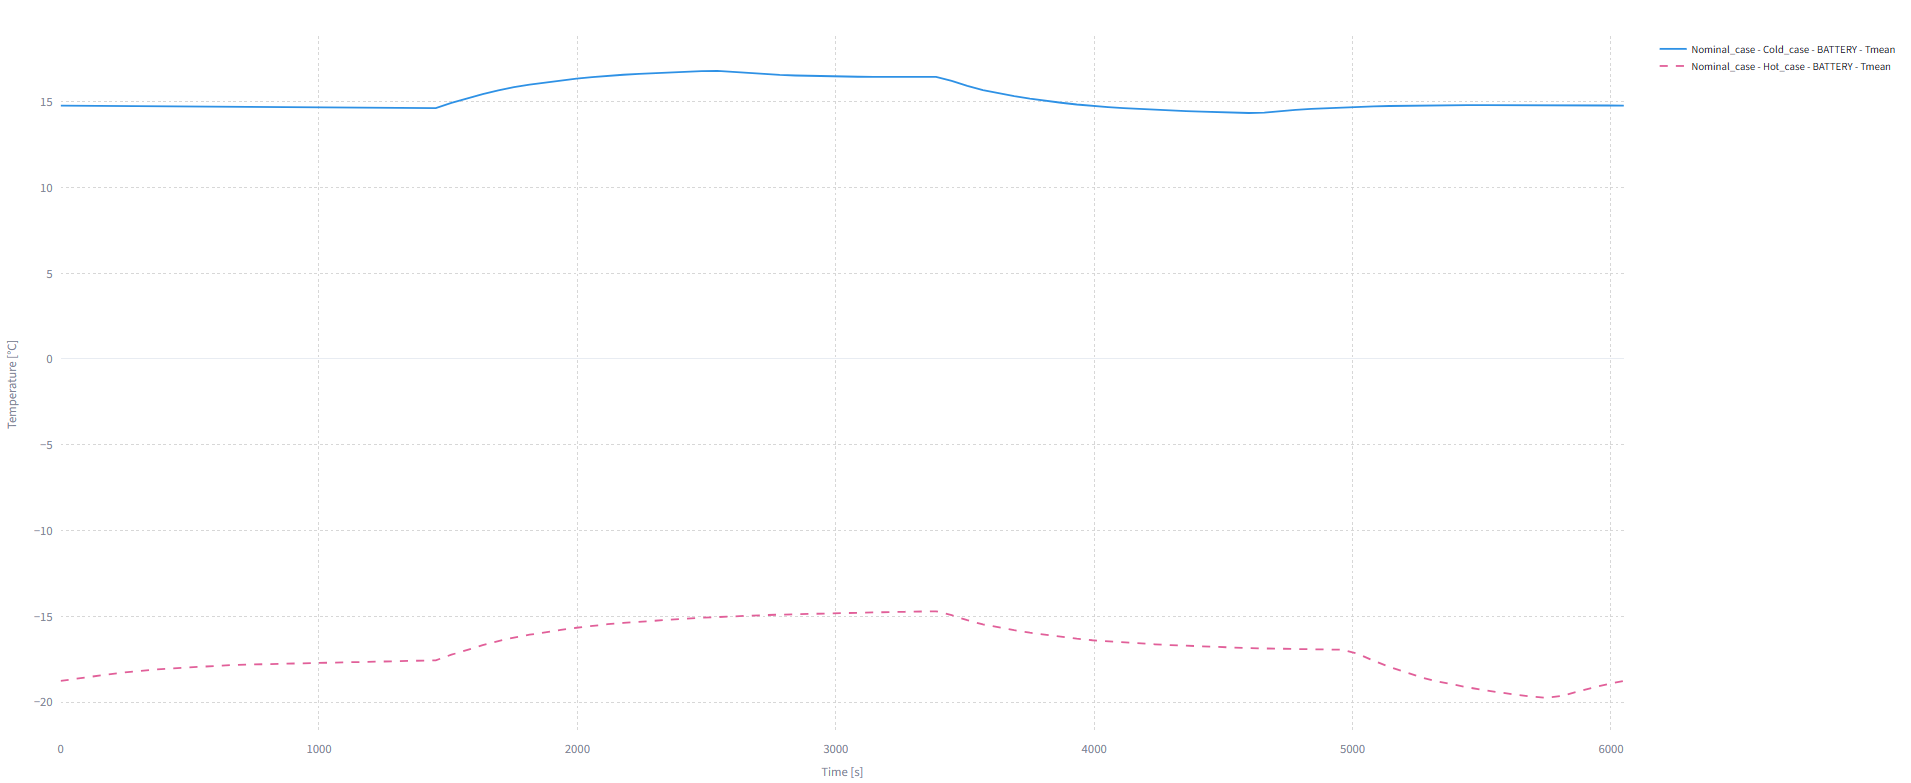
\includegraphics[
        width=1.0\textwidth,
        keepaspectratio
    ]{Figures/09/battery_temperature_difference.png}
    \caption{Nominal-minus-hot and nominal-minus-cold differences in mean
    battery temperature.}
    \label{fig:battery_temperature_difference}
\end{figure}

Table~\ref{tab:case_difference_snapshot} extends the same representation to
several groups and results at $95.80\,\mathrm{min}$. At this instant, the
nominal battery is $19.75\,^{\circ}\mathrm{C}$ colder than the hot battery
and $14.79\,^{\circ}\mathrm{C}$ warmer than the cold battery. The large
$42.96\,^{\circ}\mathrm{C}$ nominal-minus-hot difference in
\texttt{SOLAR\_PANEL\_1} occurs because the nominal panel is illuminated while
the hot case is still in eclipse. The table also separates this orbital-phase
effect from the prescribed internal dissipations: the battery load difference
is $-12.25\,\mathrm{W}$ for nominal minus hot and $1.13\,\mathrm{W}$ for
nominal minus cold.

% File: Tables/table_case_difference_snapshot.tex
% Usage: \CaseDifferenceSnapshotTable[0.98\textwidth]
% The values correspond to the selected output instant t = 95.80 min.

\newcommand{\CaseDifferenceSnapshotTable}[1][0.98\textwidth]{%
\begin{table}[H]
    \centering
    \caption{Case differences at \(t=95.80\) min, corresponding to the
    maximum absolute nominal--hot difference in mean battery temperature.}
    \label{tab:case_difference_snapshot}
    \footnotesize
    \renewcommand{\arraystretch}{1.18}
    \setlength{\tabcolsep}{3.4pt}
    \resizebox{#1}{!}{%
    \begin{tabular}{|l|c|c|c|c|c|c|}
        \hline
        & \multicolumn{3}{c|}{\textbf{Nominal -- Hot}} &
          \multicolumn{3}{c|}{\textbf{Nominal -- Cold}} \\ \cline{2-7}
        \textbf{Group} &
        \textbf{$\Delta T_{\mathrm{mean}}$ [$^\circ$C]} &
        \textbf{$\Delta Q_S$ [W]} &
        \textbf{$\Delta Q_I$ [W]} &
        \textbf{$\Delta T_{\mathrm{mean}}$ [$^\circ$C]} &
        \textbf{$\Delta Q_S$ [W]} &
        \textbf{$\Delta Q_I$ [W]} \\ \hline
        \texttt{SOLAR\_PANEL\_1} & 42.96  & 372.87 & 0.00   & 25.57 & 15.07  & 0.00  \\ \hline
        \texttt{OBC\_BOX}        & -16.33 & 4.54   & -1.00  & 12.89 & 0.18   & 2.00  \\ \hline
        \texttt{RADIATOR}         & -11.98 & 12.65  & 0.00   & 9.54  & 0.51   & 0.00  \\ \hline
        \texttt{BATTERY}          & -19.75 & 0.002  & -12.25 & 14.79 & $<0.001$ & 1.13 \\ \hline
    \end{tabular}%
    }
    \par\vspace{0.3em}
    \begin{minipage}{#1}
        \footnotesize
        \textit{Note:} Differences follow the reference-minus-comparison
        convention defined in Equation~\eqref{eq:results_case_difference}.
    \end{minipage}
\end{table}%
}

\CaseDifferenceSnapshotTable[0.8\textwidth]


\subsection{Temperature Variations and Interface Differences}
\label{subsec:temperature_interface_comparison}

The temperature-change envelopes of \texttt{BODY\_PANEL} over a nominal
$30\,\mathrm{min}$ interval are represented in
Figure~\ref{fig:body_panel_deltaT_comparison}. The effective interval obtained
from the output-time vector is $30.25\,\mathrm{min}$. Negative values identify
cooling over the selected window and positive values identify heating.

\begin{figure}[H]
    \centering
    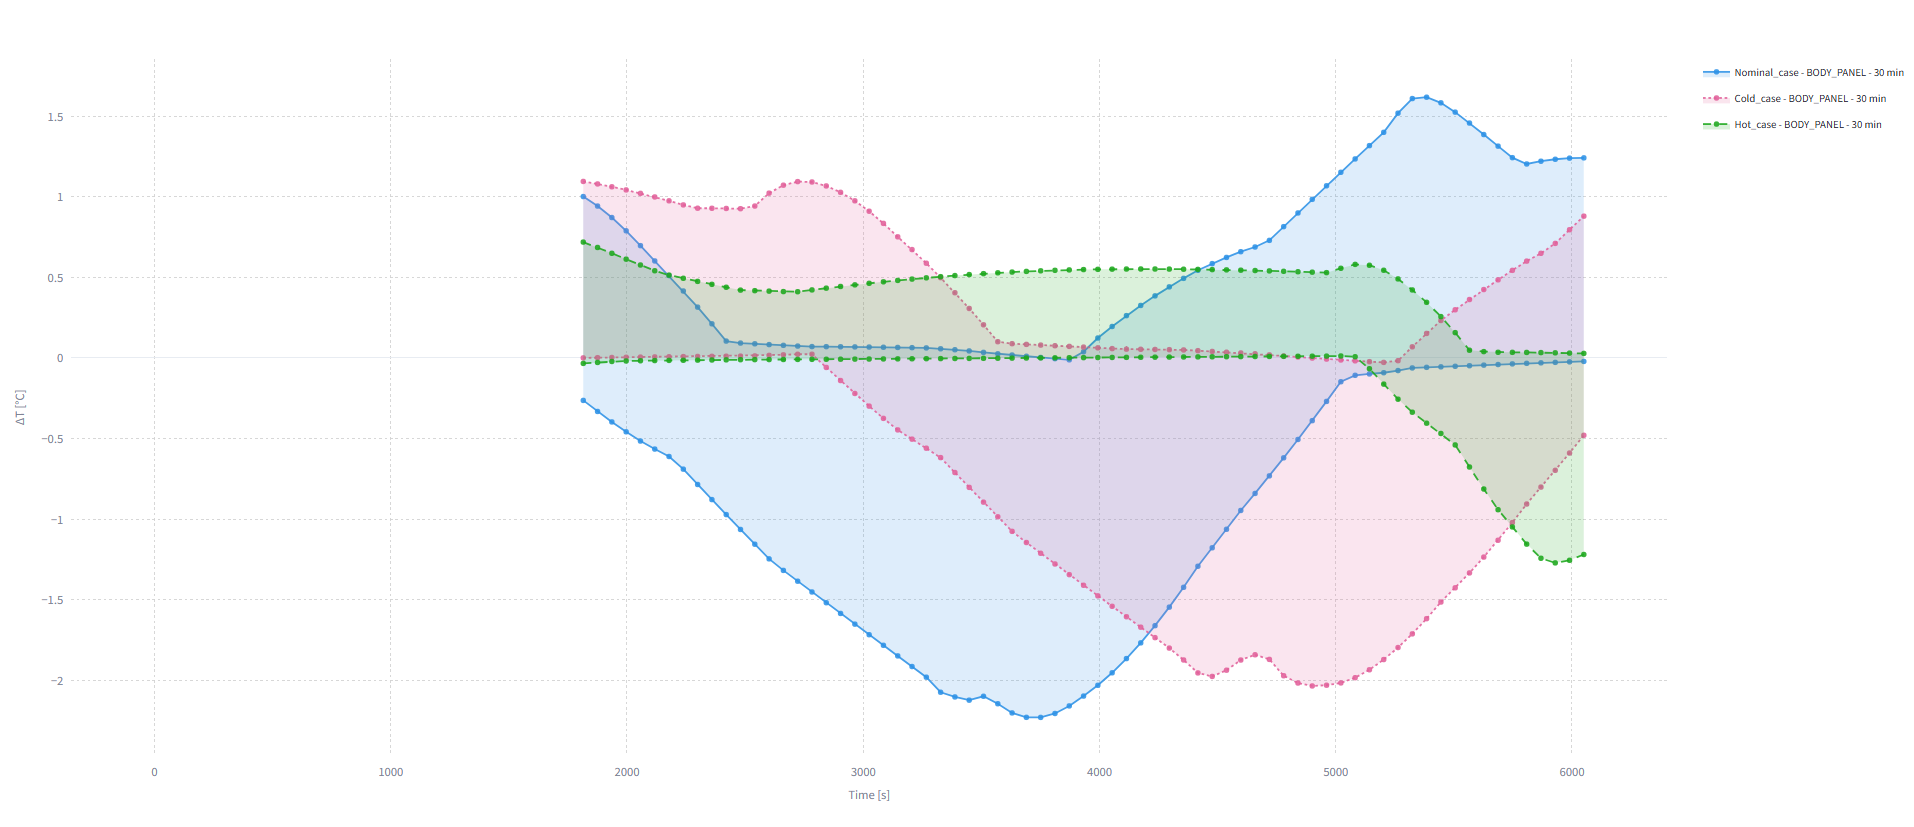
\includegraphics[
        width=0.9\textwidth,
        keepaspectratio
    ]{Figures/09/body_panel_deltaT_comparison.png}
    \caption{Temperature-change envelopes of \texttt{BODY\_PANEL} over a
    $30\,\mathrm{min}$ window.}
    \label{fig:body_panel_deltaT_comparison}
\end{figure}

The largest absolute variation occurs in the nominal case, with a decrease of
$2.23\,^{\circ}\mathrm{C}$ at $62.52\,\mathrm{min}$. The cold case reaches
$2.03\,^{\circ}\mathrm{C}$ at $81.68\,\mathrm{min}$, while the hot case
remains below $1.28\,^{\circ}\mathrm{C}$. The highest absolute temperature
case is therefore not the one with the fastest change over this interval. The
nominal and cold envelopes widen after their respective eclipse transitions,
whereas the shorter hot eclipse limits the magnitude of the delayed cooling
and reheating response.

The connected-node differences between \texttt{OBC\_BOX} and
\texttt{RADIATOR} are shown in
Figure~\ref{fig:obc_radiator_interface_comparison}. At each instant, the upper
and lower curves correspond to the connected pair that produces the largest
absolute difference for that case. The pair can change during the simulation,
so the figure is interpreted together with the maximum-value summary in
Table~\ref{tab:multicase_interface_summary}.

\begin{figure}[H]
    \centering
    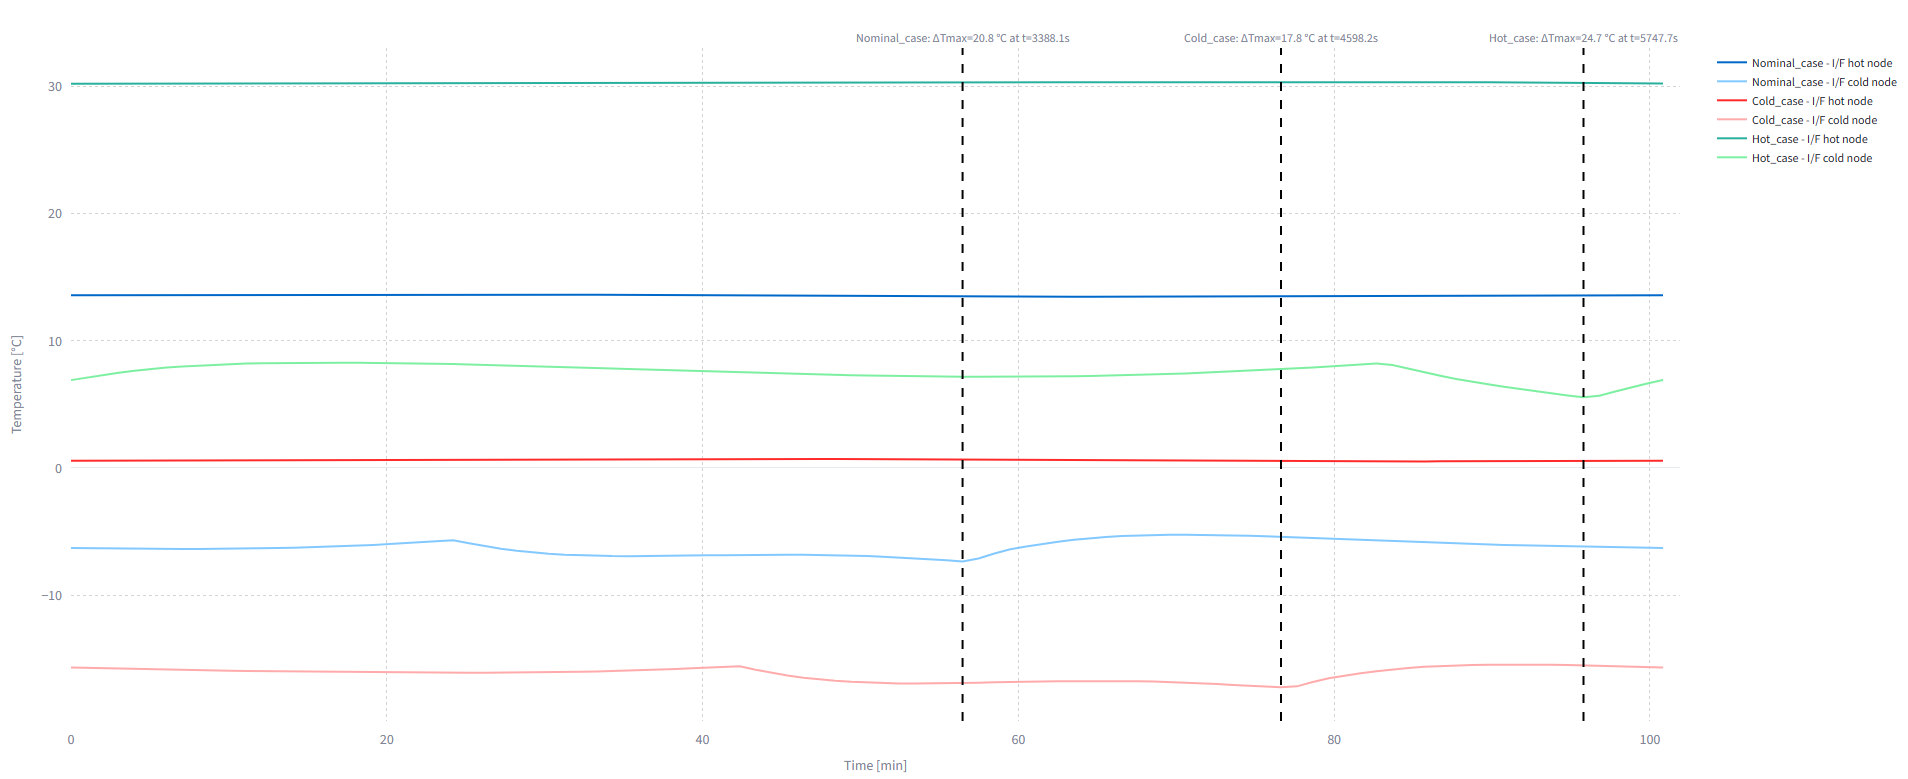
\includegraphics[
        width=0.8\textwidth,
        keepaspectratio
    ]{Figures/09/obc_radiator_interface_comparison.png}
    \caption{Critical connected-node temperatures between
    \texttt{OBC\_BOX} and \texttt{RADIATOR}.}
    \label{fig:obc_radiator_interface_comparison}
\end{figure}

% File: Tables/table_multicase_interface_summary.tex
% Usage: \MultiCaseInterfaceSummaryTable[0.98\textwidth]
% Values obtained from the OBC_BOX--RADIATOR interface exports.

\newcommand{\MultiCaseInterfaceSummaryTable}[1][0.98\textwidth]{%
\begin{table}[H]
    \centering
    \caption{Maximum connected-node temperature difference between
    \texttt{OBC\_BOX} and \texttt{RADIATOR} in the three transient cases.}
    \label{tab:multicase_interface_summary}
    \footnotesize
    \renewcommand{\arraystretch}{1.18}
    \setlength{\tabcolsep}{3.6pt}
    \resizebox{#1}{!}{%
    \begin{tabular}{|l|c|c|c|c|c|c|}
        \hline
        \textbf{Case} &
        \textbf{$|\Delta T|_{\max}$ [$^\circ$C]} &
        \textbf{Time [min]} &
        \textbf{$T_{\mathrm{hot}}$ [$^\circ$C]} &
        \textbf{$T_{\mathrm{cold}}$ [$^\circ$C]} &
        \textbf{Hot--cold nodes} &
        \textbf{Coupling} \\ \hline
        Nominal & 20.81 & 56.47 & 13.44 & -7.37  & 31023--35506 & GR \\ \hline
        Hot     & 24.67 & 95.80 & 30.22 & 5.56   & 31023--35506 & GR \\ \hline
        Cold    & 17.78 & 76.64 & 0.52  & -17.25 & 31017--35502 & GR \\ \hline
    \end{tabular}%
    }
\end{table}%
}

\MultiCaseInterfaceSummaryTable[0.98\textwidth]

The maximum interface difference increases from
$17.78\,^{\circ}\mathrm{C}$ in the cold case to
$20.81\,^{\circ}\mathrm{C}$ in the nominal case and
$24.67\,^{\circ}\mathrm{C}$ in the hot case. The nominal and hot maxima are
formed by nodes 31023 and 35506, while the cold maximum involves nodes 31017
and 35502. Both conductive and radiative couplings are present in every
critical pair. The hot environment therefore not only shifts both components
to higher temperatures, but also produces the largest separation between the
selected OBC and radiator nodes.


\subsection{Heat Flows and Net Energy Transfer}
\label{subsec:heat_flow_energy_comparison}

The total heat flow for the source--target selection \texttt{BATTERY}--
\texttt{BODY\_PLATE\_INF} follows the convention established in
Section~\ref{sec:heat_flow_evolution}. Positive values indicate heat entering
the battery from the plate, whereas negative values indicate heat leaving the
battery. Figure~\ref{fig:battery_body_plate_heat_flow_comparison} compares
$Q_{\mathrm{GT}}$ for the three cases.

\begin{figure}[H]
    \centering
    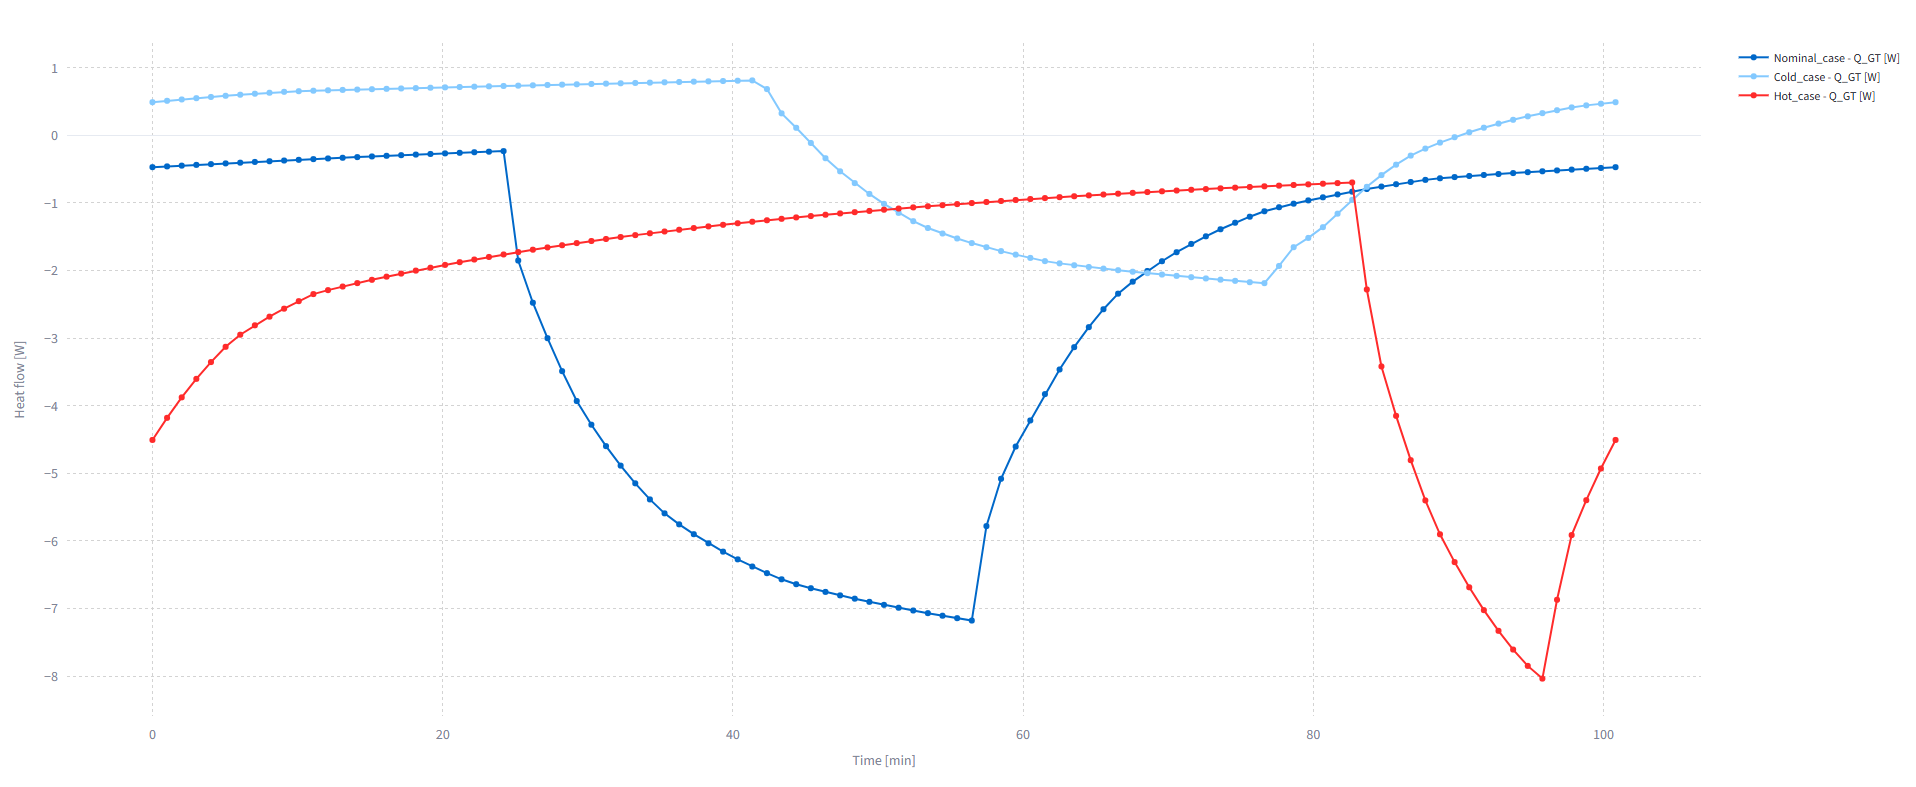
\includegraphics[
        width=0.9\textwidth,
        keepaspectratio
    ]{Figures/09/battery_body_plate_total_heat_flow_comparison.png}
    \caption{Total heat flow between \texttt{BATTERY} and
    \texttt{BODY\_PLATE\_INF}. Negative values indicate heat leaving the
    battery.}
    \label{fig:battery_body_plate_heat_flow_comparison}
\end{figure}

The nominal and hot flows remain negative throughout the interval. Their most
negative values are $-7.18\,\mathrm{W}$ and $-8.04\,\mathrm{W}$,
respectively, showing that the hotter battery continuously rejects heat to its
supporting plate. The cold case ranges from $0.81\,\mathrm{W}$ to
$-2.19\,\mathrm{W}$ and changes direction. During part of the orbit the plate
warms the battery, while the sign reverses when the battery becomes the warmer
side of the connection. In all three cases, the conductive contribution is
dominant and the radiative term only modifies the total magnitude.

The corresponding \textit{Case difference} curves are represented in
Figure~\ref{fig:battery_body_plate_heat_flow_difference}. Nominal minus hot
ranges from $-6.17$ to $7.50\,\mathrm{W}$, while nominal minus cold ranges
from $-7.19$ to $1.06\,\mathrm{W}$. The sign changes show that a single
constant offset cannot describe the effect of the environmental cases. The
relative heat transfer depends on the different eclipse intervals and on the
case-dependent battery dissipation.

\begin{figure}[H]
    \centering
    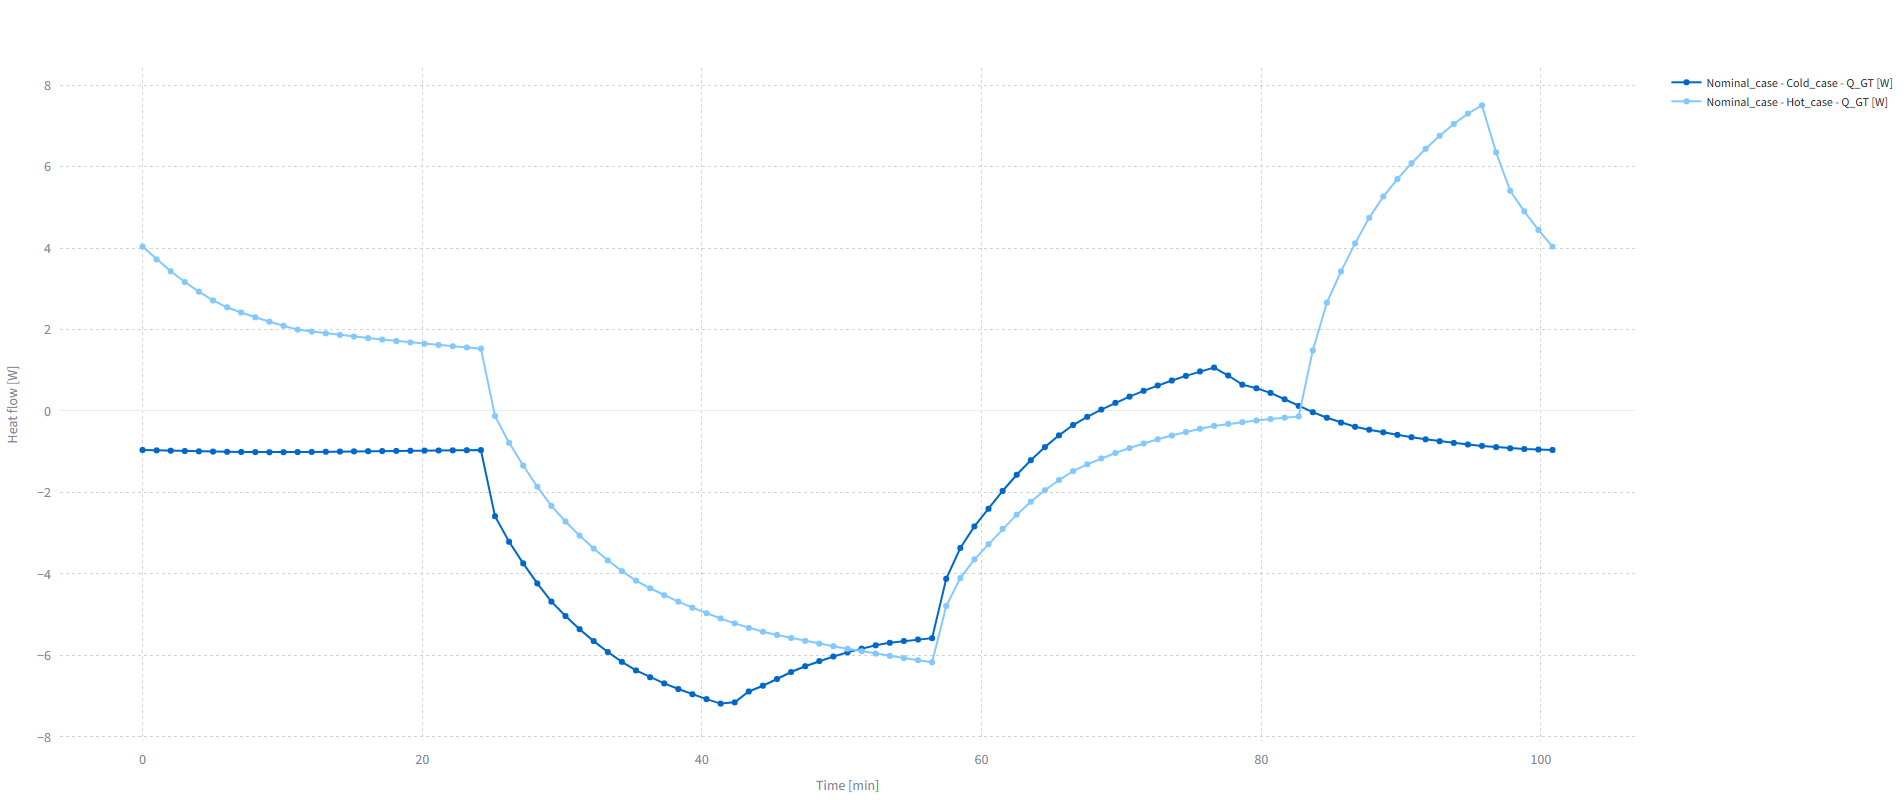
\includegraphics[
        width=0.9\textwidth,
        keepaspectratio
    ]{Figures/09/battery_body_plate_heat_flow_difference.png}
    \caption{Nominal-minus-hot and nominal-minus-cold differences in total
    battery-to-plate heat flow.}
    \label{fig:battery_body_plate_heat_flow_difference}
\end{figure}

The complete battery thermal balance and its time integral are compared in
Figure~\ref{fig:battery_net_energy_comparison}. The integral starts from zero
for each case and represents the net thermal-energy change relative to the
initial instant. It can increase or decrease according to the sign of
$Q_{\mathrm{balance}}$ and must not be interpreted as the absolute energy
stored in the battery.

\begin{figure}[H]
    \centering
    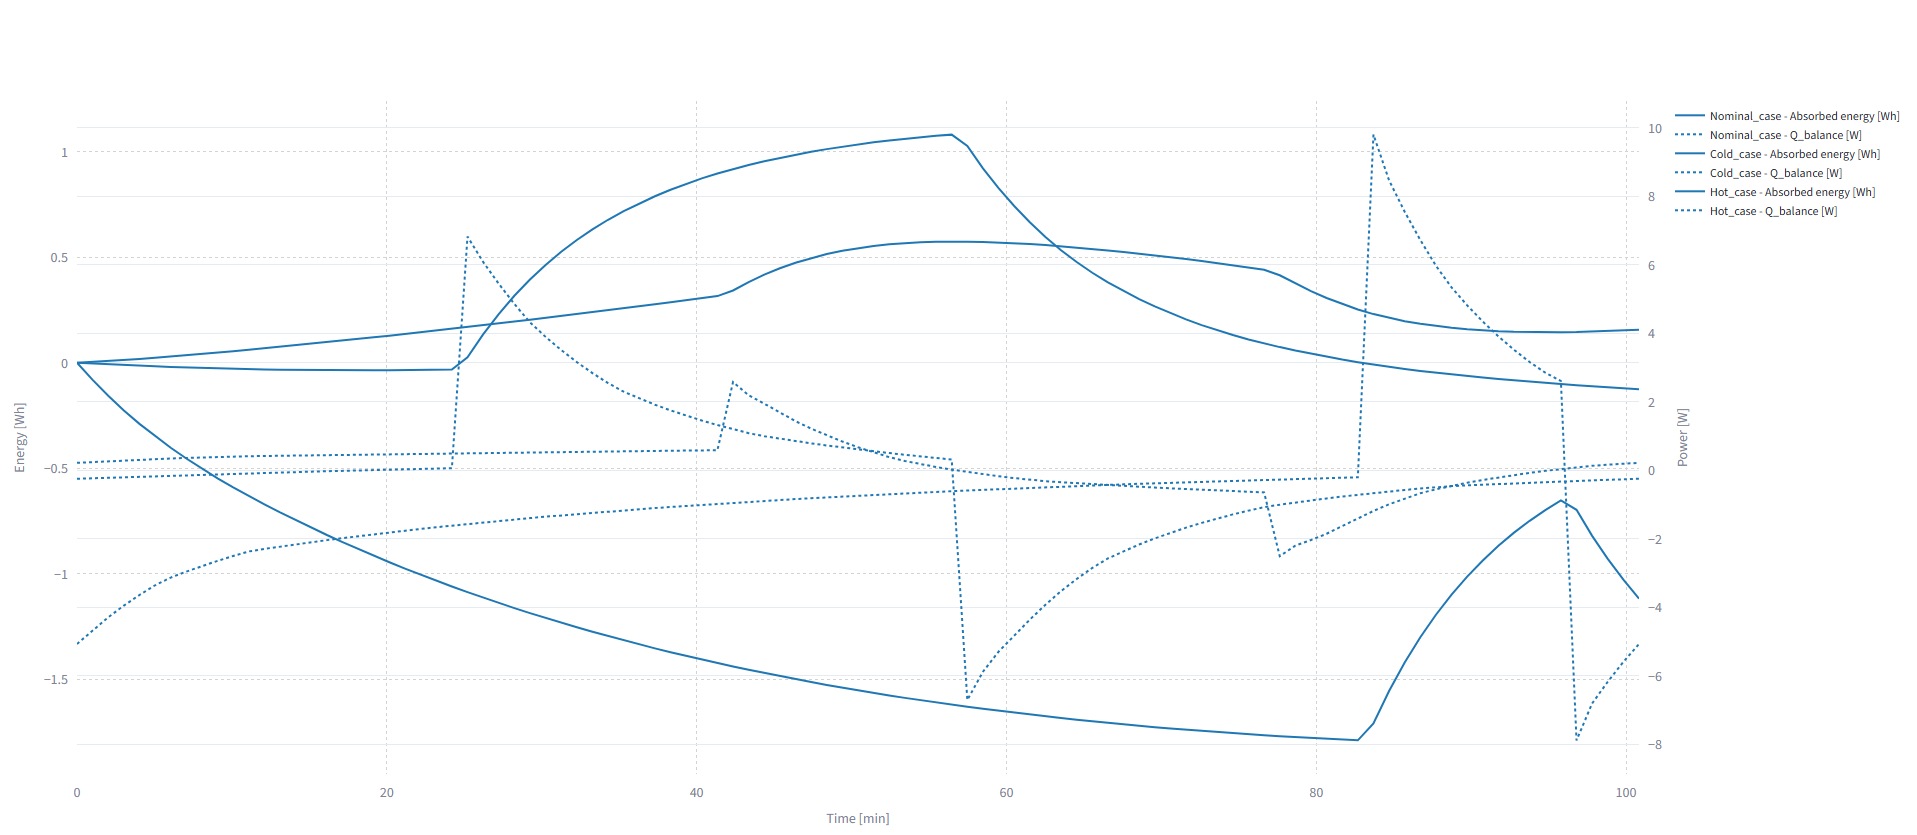
\includegraphics[
        width=0.9\textwidth,
        keepaspectratio
    ]{Figures/09/battery_net_thermal_energy_comparison.png}
    \caption{Battery thermal balance and net thermal-energy change relative to
    the initial instant.}
    \label{fig:battery_net_energy_comparison}
\end{figure}

The nominal curve initially rises to $1.08\,\mathrm{Wh}$ and subsequently
falls to $-0.13\,\mathrm{Wh}$ at the end of the simulation. The cold case
reaches $0.57\,\mathrm{Wh}$ and ends at $0.16\,\mathrm{Wh}$, indicating a
small positive net change over the analysed interval. The hot case presents a
predominantly negative integral, reaches $-1.79\,\mathrm{Wh}$ before its late
eclipse transition and finishes at $-1.12\,\mathrm{Wh}$. These values describe
the balance of all selected thermal contributions and are independent of the
electrical energy stored by the battery model.

Figure~\ref{fig:battery_thermal_balance_energy_difference} provides an
additional \textit{Case difference} example for nominal minus cold. The power
difference ranges from approximately $-6.65$ to $6.32\,\mathrm{W}$, while the
difference between their integrated thermal-energy changes remains between
$-0.35$ and $0.58\,\mathrm{Wh}$ and ends at $-0.28\,\mathrm{Wh}$. The energy
difference follows the accumulated effect of the signed power difference and
therefore varies more gradually than the instantaneous curve.

\begin{figure}[H]
    \centering
    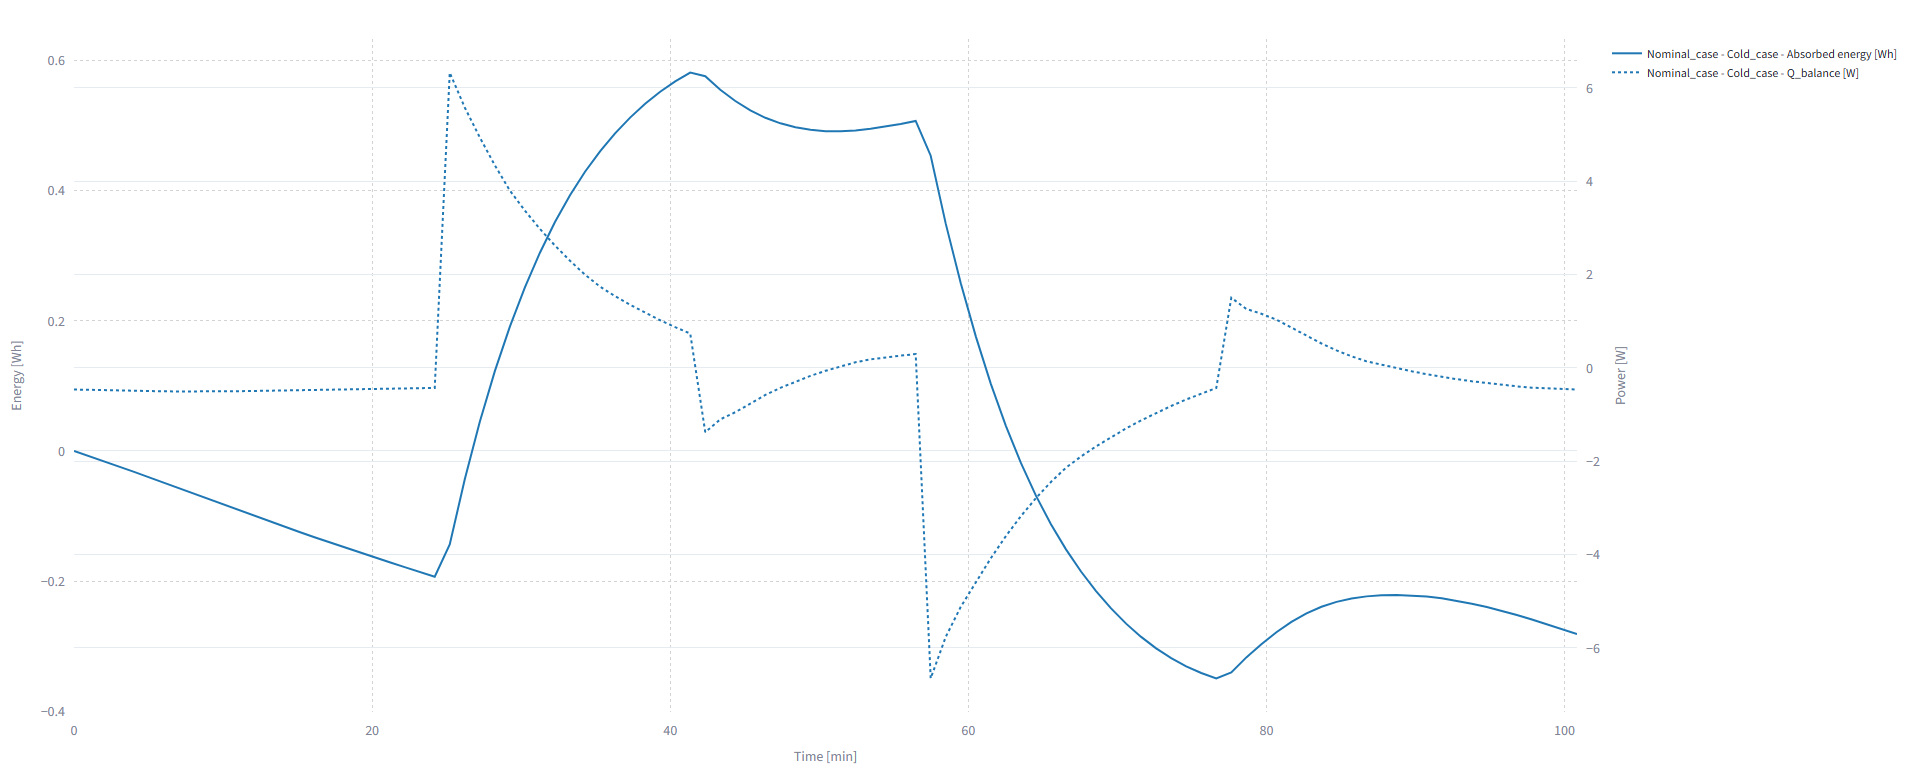
\includegraphics[
        width=0.98\textwidth,
        keepaspectratio
    ]{Figures/09/battery_thermal_balance_energy_difference.png}
    \caption{Nominal-minus-cold difference in battery thermal balance and net
    thermal-energy change.}
    \label{fig:battery_thermal_balance_energy_difference}
\end{figure}


\section{Electrical and Battery Response}
\label{sec:electrical_battery_comparison}

The same solar group, load groups, thermo-optical definition, efficiency
expression and battery parameters are used for all three cases. The electrical
comparison therefore reflects the case-dependent absorbed solar load, panel
temperature, internal dissipations and battery temperature.


\subsection{Solar Generation and Load Demand}
\label{subsec:solar_load_comparison}

Figure~\ref{fig:solar_electrical_balance_comparison} compares the estimated
solar electrical generation $Q_{S,\mathrm{elec}}$ with the demand formed by
the selected equipment groups. Generation becomes zero during the eclipse of
each case, while the load changes according to the dissipations defined in
Table~\ref{tab:internal_heat_loads}. The hot case therefore combines the
largest load with the shortest generation interruption; the cold case combines
the smallest load with the longest eclipse.

\begin{figure}[H]
    \centering
    
\includegraphics[
        width=0.9\textwidth,
        keepaspectratio
    ]{Figures/09/solar_electrical_balance_comparison.png}
    \caption{Estimated solar electrical generation and selected load demand
    in the three cases.}
    \label{fig:solar_electrical_balance_comparison}
\end{figure}

The maximum instantaneous electrical generation is
$326.25\,\mathrm{W}$ in the nominal case, $316.03\,\mathrm{W}$ in the hot
case and $317.53\,\mathrm{W}$ in the cold case. The hot case receives the
largest absorbed solar load, but its higher panel temperature reduces the
conversion efficiency and prevents it from producing the largest instantaneous
value. The total generated energy is nevertheless highest in the hot case
because of its much longer illuminated interval.

The difference curves in
Figure~\ref{fig:solar_electrical_generation_difference} are dominated by the
non-coincident eclipse intervals. Nominal minus hot falls to approximately
$-289\,\mathrm{W}$ when the nominal case enters eclipse while the hot case
remains illuminated, and later rises to about $285\,\mathrm{W}$ when the hot
case enters its late eclipse. Nominal minus cold reaches
$326\,\mathrm{W}$ after nominal illumination resumes while the cold case
remains in eclipse. When both cases share the same illumination state, the
remaining separation is associated with the different incident loads and
panel-temperature-dependent efficiencies.

\begin{figure}[H]
    \centering
    
\includegraphics[
        width=0.9\textwidth,
        keepaspectratio
    ]{Figures/09/solar_electrical_generation_difference.png}
    \caption{Nominal-minus-hot and nominal-minus-cold differences in estimated
    solar electrical generation.}
    \label{fig:solar_electrical_generation_difference}
\end{figure}

The integrated results are collected in
Table~\ref{tab:multicase_electrical_summary}. The hot case generates
$421.60\,\mathrm{Wh}$ and demands $33.75\,\mathrm{Wh}$, whereas the nominal
case generates $328.07\,\mathrm{Wh}$ and demands $25.58\,\mathrm{Wh}$. The
cold case has the lowest generation, $306.41\,\mathrm{Wh}$, but its reduced
internal loads limit the demand to $6.92\,\mathrm{Wh}$. All three direct net
balances remain positive over the complete interval. The direct deficits are
restricted to eclipse and equal $11.29\,\mathrm{Wh}$, $6.61\,\mathrm{Wh}$
and $3.24\,\mathrm{Wh}$ for the nominal, hot and cold cases, respectively.
These values are evaluated before the battery restrictions are applied.

% File: Tables/table_multicase_electrical_summary.tex
% Usage: \MultiCaseElectricalSummaryTable[0.94\textwidth]
% Energies are obtained by trapezoidal integration of the exported power
% profiles over the complete simulated interval.

\newcommand{\MultiCaseElectricalSummaryTable}[1][0.94\textwidth]{%
\begin{table}[H]
    \centering
    \caption{Integrated solar generation and selected load demand for the
    nominal, hot and cold transient cases.}
    \label{tab:multicase_electrical_summary}
    \footnotesize
    \renewcommand{\arraystretch}{1.18}
    \setlength{\tabcolsep}{4.2pt}
    \resizebox{#1}{!}{%
    \begin{tabular}{|l|c|c|c|c|c|}
        \hline
        \textbf{Case} &
        \textbf{Generated energy [Wh]} &
        \textbf{Load energy [Wh]} &
        \textbf{Direct surplus [Wh]} &
        \textbf{Direct deficit [Wh]} &
        \textbf{Net balance [Wh]} \\ \hline
        Nominal & 328.07 & 25.58 & 313.78 & 11.29 & 302.49 \\ \hline
        Hot     & 421.60 & 33.75 & 394.46 & 6.61  & 387.85 \\ \hline
        Cold    & 306.41 & 6.92  & 302.73 & 3.24  & 299.49 \\ \hline
    \end{tabular}%
    }
    \par\vspace{0.3em}
    \begin{minipage}{#1}
        \footnotesize
        \textit{Note:} Direct surplus and deficit are the time integrals of
        the positive and negative parts, respectively, of
        \(Q_{S,\mathrm{elec}}-Q_{\mathrm{load}}\), before applying the battery
        operating limits.
    \end{minipage}
\end{table}%
}

\MultiCaseElectricalSummaryTable[0.85\textwidth]


\subsection{Battery State and Operating Limits}
\label{subsec:battery_comparison}

Battery operation is calculated independently for each physical case. Direct
subtraction is not used for SOC, voltage or current because the difference
between two battery states does not describe an independent operating state.
The absolute SOC curves in Figure~\ref{fig:battery_soc_comparison} provide the
main comparison.

\begin{figure}[H]
    \centering
    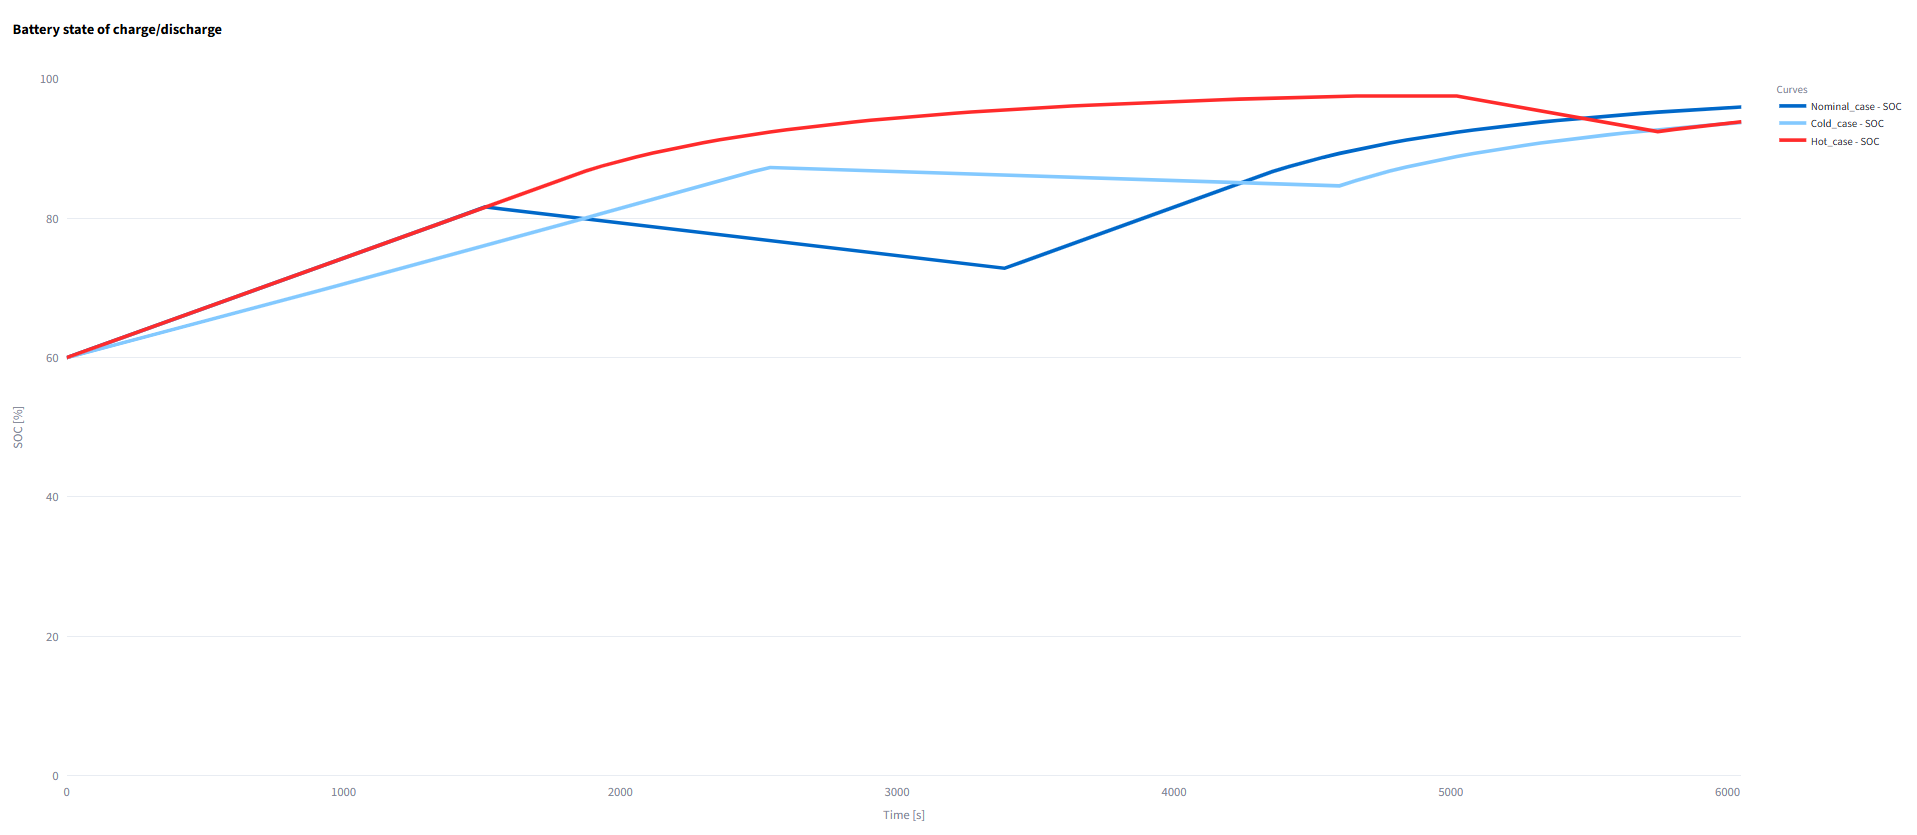
\includegraphics[
        width=0.82\textwidth,
        keepaspectratio
    ]{Figures/09/battery_soc_comparison.png}
    \caption{Battery state of charge obtained with the common battery
    configuration.}
    \label{fig:battery_soc_comparison}
\end{figure}

All cases begin at $60\%$ SOC. The nominal battery charges before eclipse,
discharges while solar generation is absent and subsequently recovers to a
final value of $94.43\%$. The cold battery follows the same sequence with a
longer discharge interval but a substantially lower demand, ending at
$93.08\%$. The hot battery reaches the largest maximum SOC,
$97.56\%$, before its late eclipse. Its higher eclipse load then causes the
strongest discharge and the remaining illuminated interval only restores the
SOC to $90.84\%$. Final SOC therefore depends on the timing of generation and
demand as well as on their total integrated values.

The battery temperatures and thermal charging restrictions are compared in
Figure~\ref{fig:battery_temperature_derating_comparison}. Charge and discharge
efficiencies remain fixed at $0.98$ in all cases. The nominal and hot battery
temperatures remain inside the unrestricted charging interval, so their
charge-derating factors stay equal to one. The cold battery remains between
$3.66$ and $4.46\,^{\circ}\mathrm{C}$, inside the lower $5\,^{\circ}\mathrm{C}$
derating ramp. Its factor varies from $0.733$ to $0.892$ and restricts charging
throughout the complete $100.84\,\mathrm{min}$ simulation.

\begin{figure}[H]
    \centering
    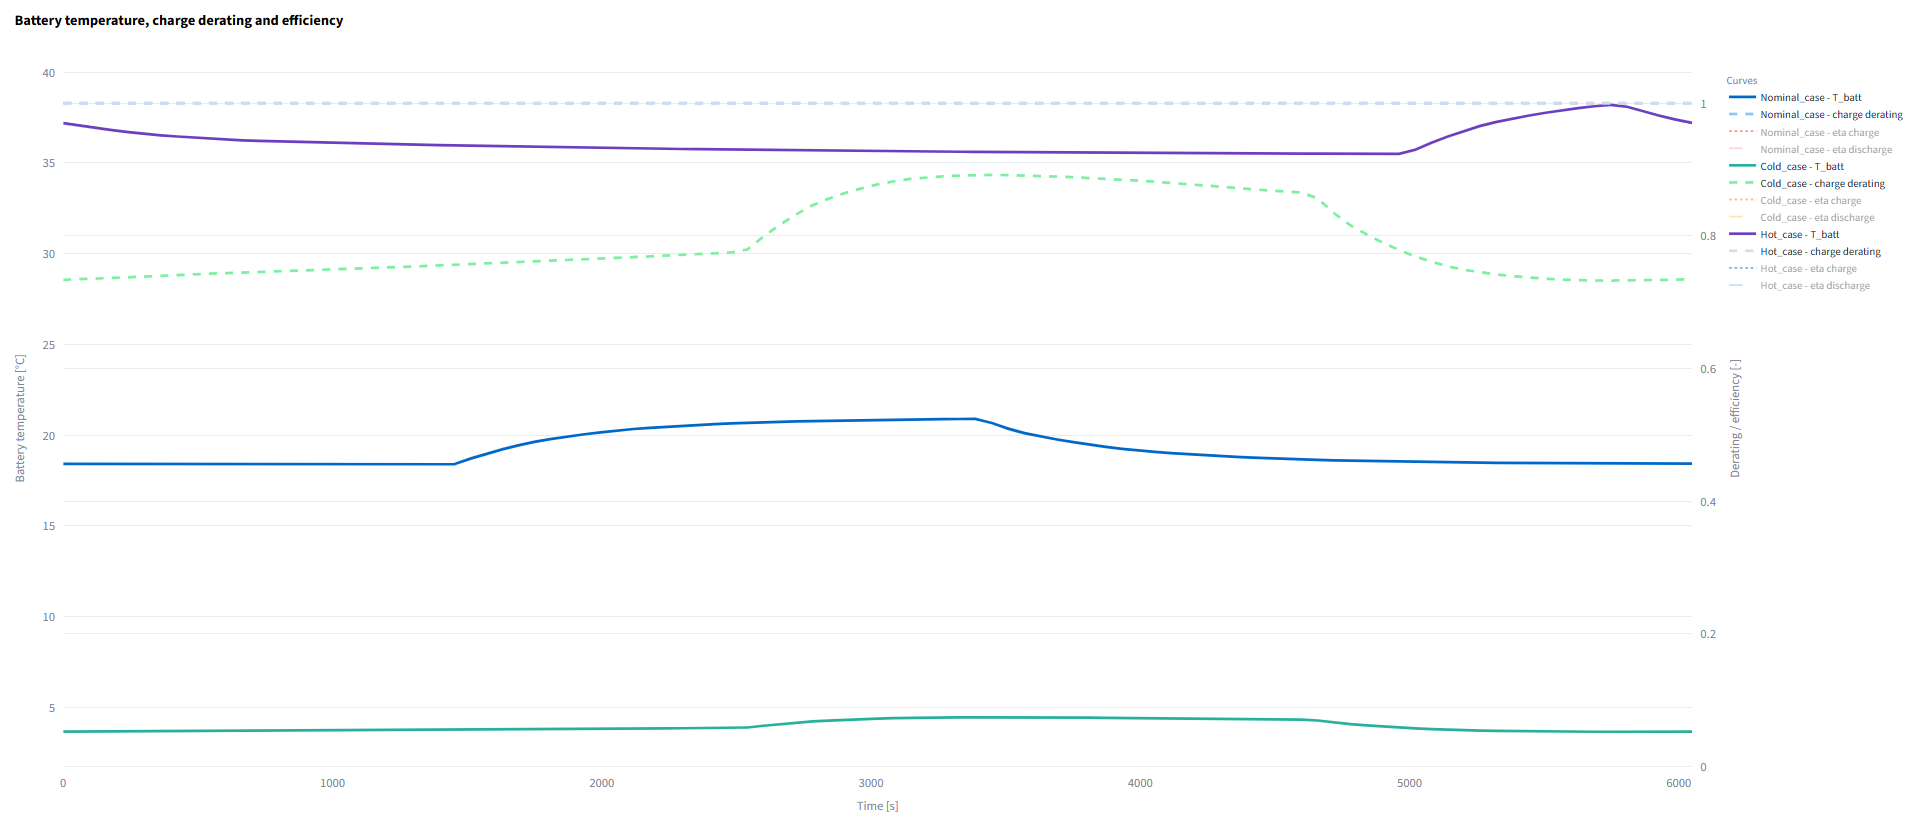
\includegraphics[
        width=0.85\textwidth,
        keepaspectratio
    ]{Figures/09/battery_temperature_derating_comparison.png}
    \caption{Battery temperature, charge-derating factor and electrical
    efficiencies in the three cases.}
    \label{fig:battery_temperature_derating_comparison}
\end{figure}

The lower accepted charge current limits the cold-case maximum charge power to
$30.24\,\mathrm{W}$, compared with approximately $35.4\,\mathrm{W}$ in the
nominal and hot cases. Despite this restriction, the available generation and
stored energy remain sufficient to supply the complete selected load. The
unserved-load energy is negligible in every simulation.

Terminal voltage and charge/discharge currents are shown separately in
Figure~\ref{fig:battery_voltage_current_comparison} to avoid overlapping nine
curves in a single graph. The same battery parameters and axis definitions are
retained in the three subfigures.

\begin{figure}[H]
    \centering

    \begin{subfigure}[t]{0.85\textwidth}
        \centering
        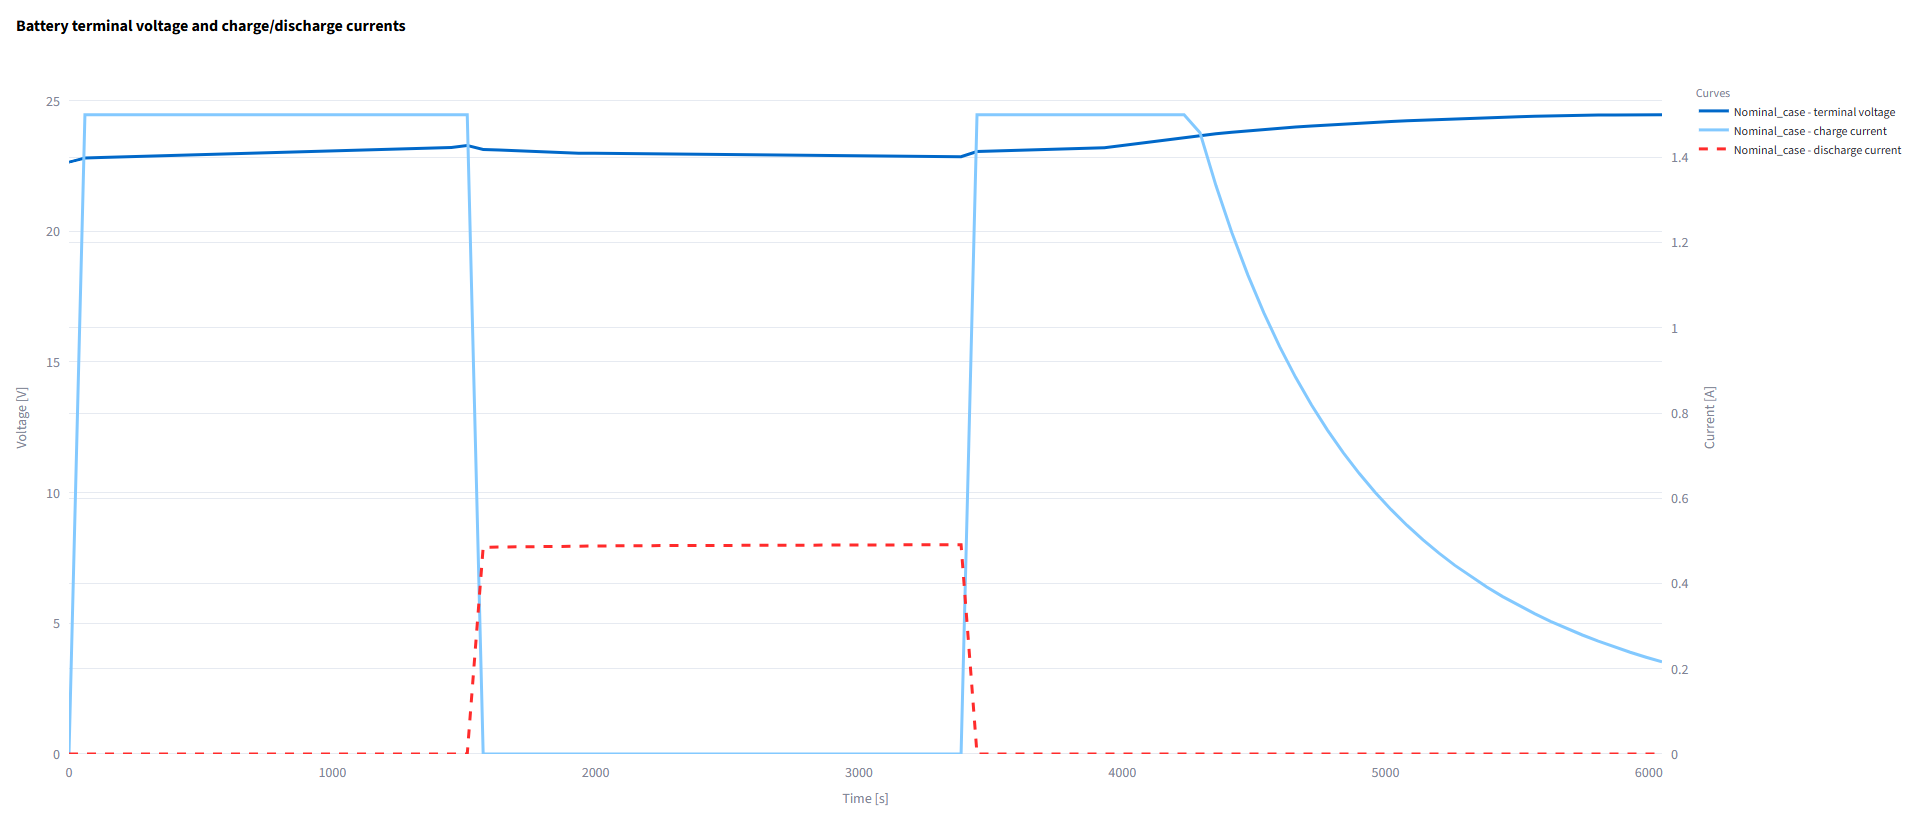
\includegraphics[
            width=\textwidth,
            keepaspectratio
        ]{Figures/09/nominal_battery_voltage_current.png}
        \caption{Nominal case.}
        \label{fig:nominal_battery_voltage_current_ch9}
    \end{subfigure}
\end{figure}

\begin{figure}[H]
    \ContinuedFloat
    \centering

    \begin{subfigure}[t]{0.8\textwidth}
        \centering
        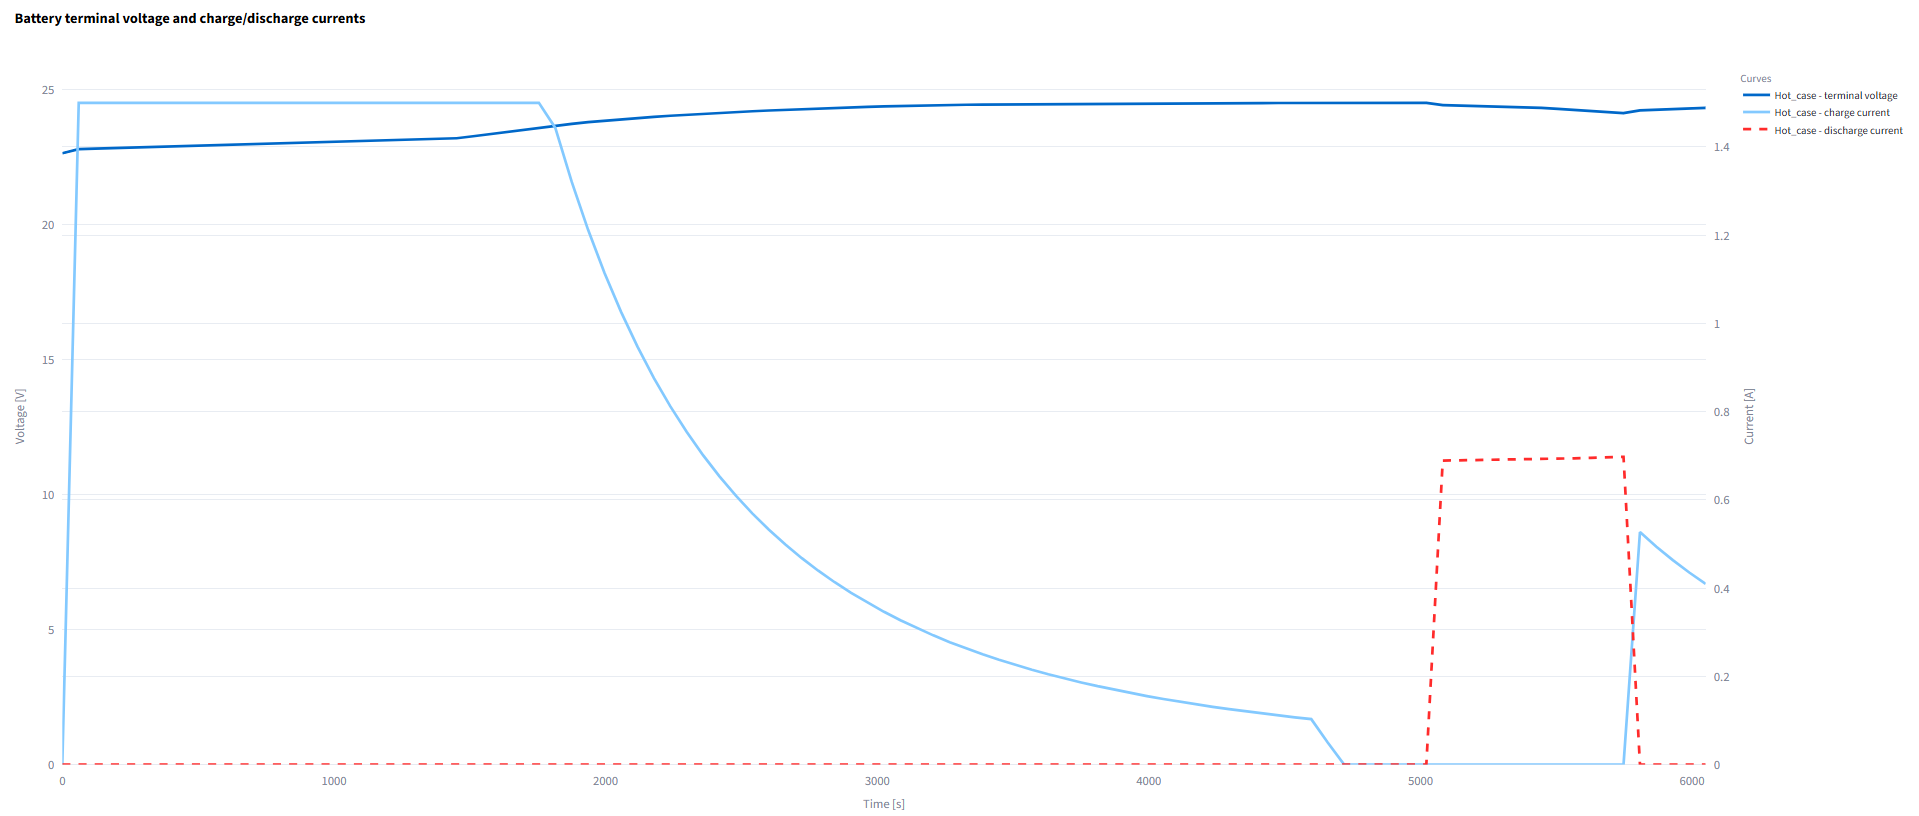
\includegraphics[
            width=\textwidth,
            keepaspectratio
        ]{Figures/09/hot_battery_voltage_current.png}
        \caption{Hot case.}
        \label{fig:hot_battery_voltage_current_ch9}
    \end{subfigure}

\end{figure}

\begin{figure}[H]
    \ContinuedFloat
    \centering

    \begin{subfigure}[t]{0.74\textwidth}
        \centering
        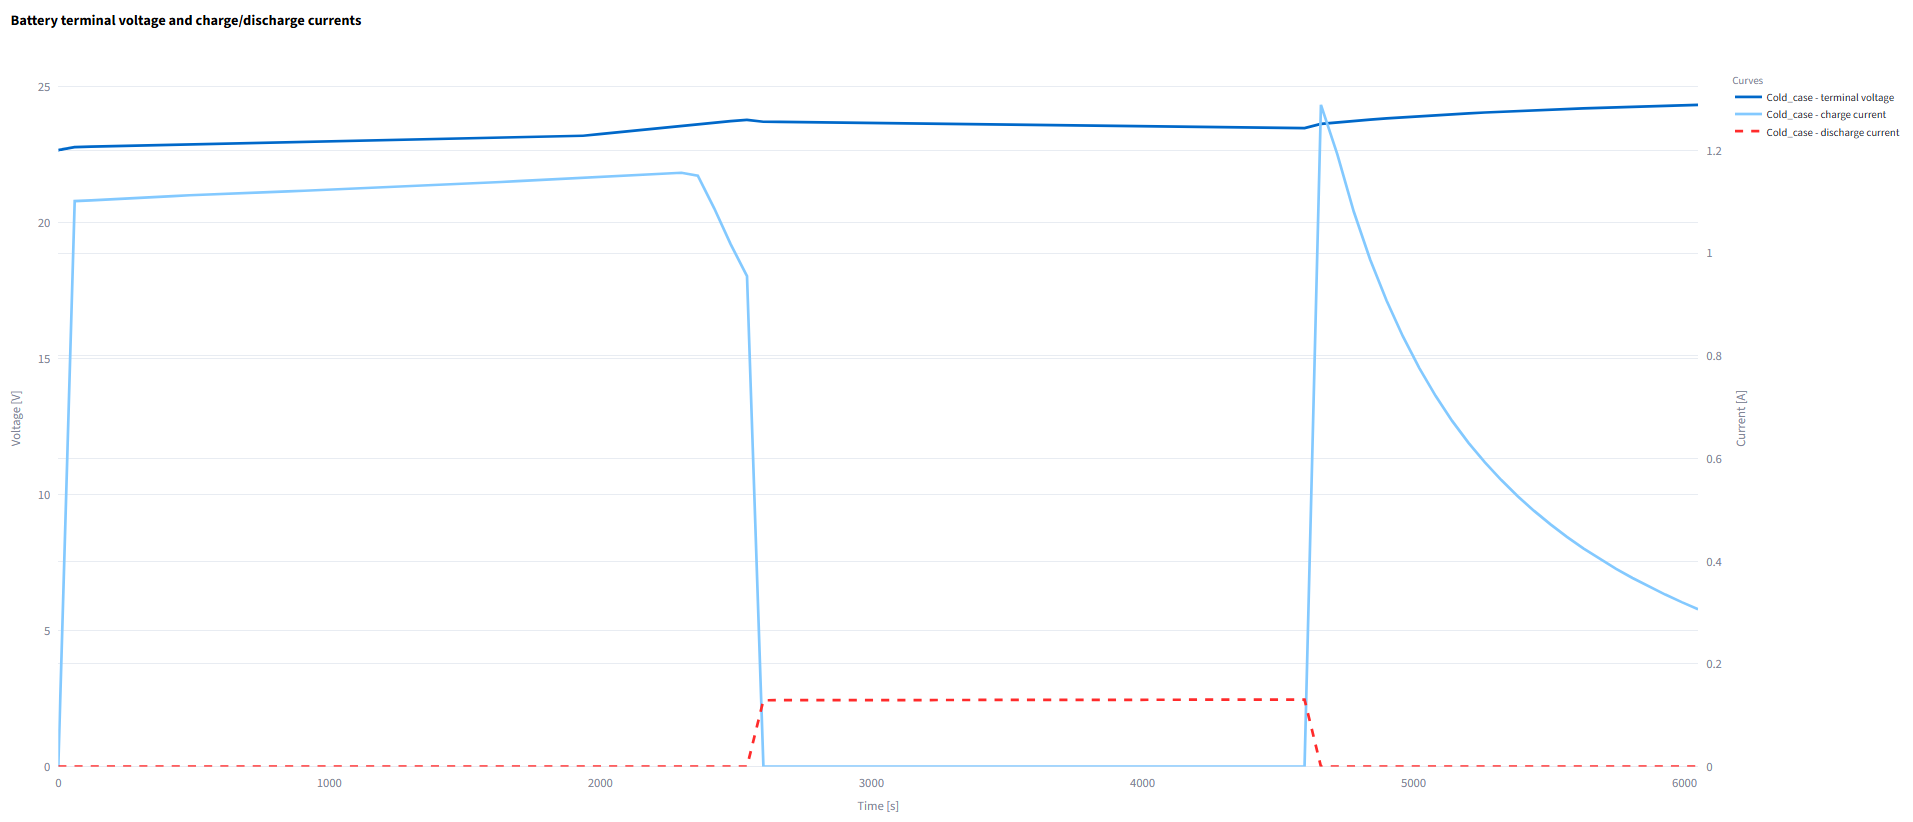
\includegraphics[
            width=\textwidth,
            keepaspectratio
        ]{Figures/09/cold_battery_voltage_current.png}
        \caption{Cold case.}
        \label{fig:cold_battery_voltage_current_ch9}
    \end{subfigure}

    \caption{Battery terminal voltage and charge/discharge currents for the
    nominal, hot and cold transient cases.}
    \label{fig:battery_voltage_current_comparison}    
\end{figure}

\FloatBarrier

% File: Tables/table_multicase_battery_summary.tex
% Usage: \MultiCaseBatterySummaryTable[0.86\textwidth]
% Values obtained from the joint battery-summary export.

\newcommand{\MultiCaseBatterySummaryTable}[1][0.86\textwidth]{%
\begin{table}[H]
    \centering
    \caption{Main battery results for the nominal, hot and cold transient
    cases using the common battery configuration.}
    \label{tab:multicase_battery_summary}
    \footnotesize
    \renewcommand{\arraystretch}{1.30}
    \setlength{\tabcolsep}{4.8pt}
    \begin{tabularx}{#1}{
        |>{\raggedright\arraybackslash}X
        |>{\centering\arraybackslash}c
        |>{\centering\arraybackslash}c
        |>{\centering\arraybackslash}c
        |>{\centering\arraybackslash}c|
    }
        \hline
        \textbf{Result} &
        \textbf{Nominal} &
        \textbf{Hot} &
        \textbf{Cold} &
        \textbf{Unit} \\ \hline
        Final state of charge
        & 95.98 & 93.87 & 93.75 & \% \\ \hline
        Minimum state of charge
        & 60.00 & 60.00 & 60.00 & \% \\ \hline
        Maximum state of charge
        & 95.98 & 97.56 & 93.75 & \% \\ \hline
        Maximum charge power
        & 35.39 & 35.40 & 30.42 & W \\ \hline
        Maximum discharge power
        & 11.22 & 16.84 & 3.06 & W \\ \hline
        Battery-temperature range
        & 18.40--20.90 & 35.50--38.20 & 3.66--4.46 & $^\circ$C \\ \hline
        Minimum charge-derating factor
        & 1.000 & 1.000 & 0.733 & -- \\ \hline
        Charge-derated duration
        & 0.00 & 0.00 & 100.84 & min \\ \hline
        Curtailed solar energy
        & 282.51 & 368.19 & 275.99 & Wh \\ \hline
        Unserved-load energy
        & $\approx 0$ & $\approx 0$ & $\approx 0$ & Wh \\ \hline
    \end{tabularx}
\end{table}%
}
\MultiCaseBatterySummaryTable[0.7\textwidth]

The nominal voltage ranges from $22.65$ to $24.38\,\mathrm{V}$, with maximum
charge and discharge currents of $1.50$ and $0.95\,\mathrm{A}$. The hot case
reaches $24.52\,\mathrm{V}$ and the largest discharge current,
$1.30\,\mathrm{A}$, consistently with its $30.87\,\mathrm{W}$ maximum
discharge power. The cold case reaches $24.25\,\mathrm{V}$, while its maximum
charge and discharge currents remain at $1.29$ and $0.24\,\mathrm{A}$. The
reduced cold-case current is consistent with both the lower selected load and
the active charge derating.

The summary confirms that no case reaches the lower SOC limit or leaves
electrical demand unserved. The hot case produces the largest curtailed solar
energy, $364.18\,\mathrm{Wh}$, because its high generation frequently exceeds
the power and current accepted by the battery. The nominal and cold values are
similar, $276.23$ and $274.51\,\mathrm{Wh}$, although the physical causes
differ: the nominal battery is unrestricted thermally, while the cold battery
rejects additional surplus because of its reduced charge capability.


\section{Overall Comparison}
\label{sec:overall_comparison}

The selected cases provide the expected upper and lower thermal environments
without changing the common model architecture. The hot case produces the
highest equipment temperatures and the largest OBC--radiator interface
difference, while the cold case produces the lowest temperatures and activates
the battery charge derating. The nominal solution generally remains between
both limits, although differences in eclipse timing can temporarily reverse
the ordering of solar-panel temperatures, loads and heat flows.

The transient comparisons also show that absolute temperature, temporal
variation and spatial non-uniformity are separate results. The hot case has the
highest temperatures but the smallest $30\,\mathrm{min}$ variation of
\texttt{BODY\_PANEL}; the cold battery has the lowest temperature but also the
smallest internal battery range. Interface and flow results similarly depend
on the local connection and can change node pair, magnitude or direction
between cases.

The electrical response is governed by both illumination and temperature.
Higher panel temperature reduces instantaneous conversion efficiency, whereas
eclipse duration controls the total generated energy and the discharge
interval. The hot case consequently generates the most energy but ends with
the lowest final SOC because its high load and late eclipse produce the
strongest discharge near the end of the simulation. The cold case receives
the least solar energy and remains thermally derated, but its reduced demand
prevents unserved load and allows the battery to finish above $93\%$ SOC.

The combined results confirm the value of retaining both superposed curves and
\textit{Case difference}. Absolute representations preserve the operating
levels required to assess temperatures, flows and battery limits, while the
difference mode quantifies the separation from the nominal solution and makes
the influence of non-coincident orbital events directly visible.

\FloatBarrier

\cleardoublepage

\chapter{Conclusions and Future Work}
\label{ch:conclusions_future_work}

\section{Conclusions}
\label{sec:conclusions}

The developed application meets the main objective of processing, analysing
and comparing several transient cases associated with the same
\acrshort{esatan-tms} thermal model. The initial steady-state tool has been
extended without removing its previous inspection capabilities, providing a
common environment for examining complete time series and results at selected
instants.

A representative spacecraft thermal model has been developed to support the
implementation and evaluation of these functions. The nominal, hot and cold
cases retain the same geometry, node hierarchy, materials and thermal
connections, while the environmental conditions and internal dissipations are
modified. This common basis allows equivalent groups, nodes and exported
result fields to be compared directly throughout the simulated interval.

The application can load several compatible result files, preserve their case
identity and apply the same selection to all of them. Transient temperatures,
thermal loads, conductive and radiative heat flows, interface temperature
differences and time-integrated energy transfers can be represented using
superposed curves. The \textit{Case difference} option complements these
absolute results by calculating the separation between a reference case and
one or more comparison cases. Together, both representations preserve the
physical operating levels and make smaller differences or non-coincident
orbital events easier to identify.

Additional calculations extend the imported \acrshort{esatan-tms} results.
Temperature changes can be evaluated over selected time windows, critical
interfaces are identified from explicit thermal connections and summary tables
condense the main extrema and their occurrence times. Analyses and their
configurations can also be saved, restored and exported, reducing the need to
repeat the complete selection process when the same result must be examined
again.

The thermal post-processing is complemented by an electrical analysis based on
the selected solar-panel and internal-load results. The absorbed solar load is
used to estimate incident and converted electrical power, while the selected
internal dissipations provide an approximation of the electrical load demand.
These profiles supply a separate battery model that calculates state of charge,
terminal voltage, current, accepted and curtailed power, conversion and
resistive losses, and temperature-dependent operating restrictions. All these
results are obtained during post-processing and do not modify the original
thermal solution.

The comparison of the three cases confirms that the highest absolute
temperature does not necessarily coincide with the largest temporal variation
or the greatest local gradient. The hot case produces the highest equipment
temperatures and the largest OBC--radiator interface difference, whereas the
cold case produces the lowest battery temperature and activates the charging
derating. Differences in eclipse timing also affect solar generation, load
support and the final battery state.

The hot case generates the greatest electrical energy but finishes with the
lowest state of charge because its late eclipse and higher demand produce the
strongest final discharge. The cold case receives less solar energy and
remains thermally restricted, although its lower load prevents unserved
demand. These results show that battery operation cannot be determined from
the generated or demanded energy alone, since their temporal distribution and
the active operating limits are also relevant.

The resulting tool therefore connects transient thermal inspection,
multi-case comparison and a simplified electrical interpretation within the
same workflow. It does not replace the thermal solver or constitute a complete
spacecraft electrical-power-system model. Its purpose is to organise the
exported results, reproduce consistent analyses and reveal the relations
between environmental conditions, thermal response, electrical generation and
battery operation. The modular structure also provides a suitable basis for
further extensions without requiring the existing analysis areas to be
redesigned.


\section{Future Work}
\label{sec:future_work}


The following lines extend the current physical models, analysis capabilities
and software architecture without changing the scope of the completed
implementation.

\begin{itemize}[
    leftmargin=*,
    itemsep=0.9em,
    topsep=0.5em,
    parsep=0pt
]
    \item \textbf{Battery-model extension.}
    The current implementation is a configurable post-processing approximation
    based on a generic piecewise voltage curve, separate charge and discharge
    resistances and a simplified CC--CV strategy. Greater physical fidelity
    would require voltage--SOC curves calibrated for a specific cell, different
    charge and discharge characteristics, temperature-dependent resistance and
    usable capacity, hysteresis and dynamic RC branches. Ageing,
    cycle-dependent capacity loss and validation against experimental or
    manufacturer data would also allow the calculated voltage, current and
    state of charge to be evaluated for a defined battery technology.

    \item \textbf{Bidirectional thermal--electrical coupling.}
    The thermal and electrical calculations currently follow a one-directional
    sequence: thermal results determine solar generation, load demand and
    battery operation, but the calculated electrical losses are not returned
    to the thermal model. A bidirectional procedure could convert battery
    resistive losses, conversion losses and operating-mode changes into
    time-dependent heat loads for a subsequent \acrshort{esatan-tms} solution.
    An iterative exchange between both models would provide a more consistent
    thermo-electrical response without requiring the post-processing
    application to replace the thermal solver.

    \item \textbf{Comparison between different thermal-model architectures.}
    Multi-case comparison is presently restricted to result files that share a
    common node hierarchy. A further extension could compare successive
    versions or different architectures of the same thermal model by defining
    correspondences between equivalent groups and components. The comparison
    would then identify common elements, warn about unmatched regions and
    normalise selected results by properties such as area, mass or thermal
    capacitance when a direct nodal subtraction is not meaningful.

    \item \textbf{Alignment by orbital events.}
    Temporal alignment by eclipse entry, eclipse exit or orbital phase would
    permit comparisons between simulations with different starting instants or
    output-time vectors. This option would separate the effect of the physical
    event from a displacement in the simulation timeline and facilitate the
    comparison of cases with different eclipse durations.

    \item \textbf{Sensitivity and uncertainty analysis.}
    The existing multi-case framework provides a basis for sensitivity and
    uncertainty studies. Sets of cases could be generated by varying contact
    conductances, thermo-optical properties, internal dissipations, orbital
    conditions or electrical parameters. Automated envelopes, uncertainty
    bands and rankings would identify the inputs with the greatest influence on
    each component.

    \item \textbf{Automatic critical-event detection.}
    The same process could detect temperature-limit violations, maximum case
    differences, rapid thermal variations, changes in heat-flow direction,
    minimum state of charge, active derating and periods of unserved load. A
    common event table could then identify the affected case, element, time and
    result without requiring every curve to be inspected individually.

    \item \textbf{Performance and scalability.}
    Larger thermal models and broader collections of transient cases would
    benefit from selective loading of required result fields, deferred
    processing, reuse of intermediate calculations and parallel execution
    between cases. These improvements could reduce memory use and response time
    when processing long simulations, finer temporal discretisations or a
    large number of result files.

    \item \textbf{Batch processing and automatic report generation.}
    A batch mode could apply a saved analysis configuration to an entire folder
    of cases and export the corresponding plots, tables and numerical
    summaries. Report templates for LaTeX, PDF or spreadsheet formats would
    extend this process towards reproducible and partially automated result
    documentation.

    \item \textbf{Persistent-storage improvements.}
    Metadata, widget configurations and generated files are currently
    coordinated between a local database and output folders. A unified
    transactional layer could prevent incomplete records, detect orphaned
    files and avoid unnecessary duplication. Portable analysis packages would
    allow complete configurations to be exported, transferred and restored on
    another installation. Version information and migration rules would
    preserve compatibility when the application structure or available
    controls change.

    \item \textbf{Dedicated web architecture.}
    The interface may evolve from Streamlit towards a separate frontend based
    on HTML, CSS and JavaScript, connected to a Python backend through an
    application programming interface. This architecture would offer greater
    control over layout, asynchronous calculations, user sessions and remote
    deployment while retaining the calculation modules as an independent
    backend.

    \item \textbf{Automated testing and validation.}
    Unit, integration and regression tests could check file loading, sign
    conventions, numerical integration, multi-case differences, battery
    calculations and saved-analysis restoration after each software change.
    These tests would also provide a stable basis for introducing new result
    formats, analysis modules and physical models.
\end{itemize}

\cleardoublepage

%   ---   BIBLIOGRAFÍA/REFERENCIAS   ---   %
%\nocite{*}
\chapter*{References}
\addcontentsline{toc}{chapter}{References}
\bibliographystyle{elsarticle-num}
\bibliography{references.bib}
\cleardoublepage
%\chapter{References}
%\phantomsection % Para que el capítulo aparezca en el índice
% comando para eliminar el número de sección del capítulo de referencias
%\addcontentsline{toc}{section}{Referencias}
%\renewcommand{\refname}{Referencias}
%\bibliographystyle{elsarticle-num}
%\bibliography{references.bib}
%\cleardoublepage

%   ---   ANEXOS   ---   %

\appendix
\hiddenappendixchapter
    {Application Launch and Interface Overview}
    {app:application_interface_overview}

\section{Inspection and Conductor Modules}
\label{appsec:inspection_modules}

The model-inspection and conductor-analysis tabs follow the general interface
organisation described in Chapter~6. The following views show each area
separately so that its main selectors, controls and output regions can be
identified clearly.

\begin{figure}[p]
    \centering
    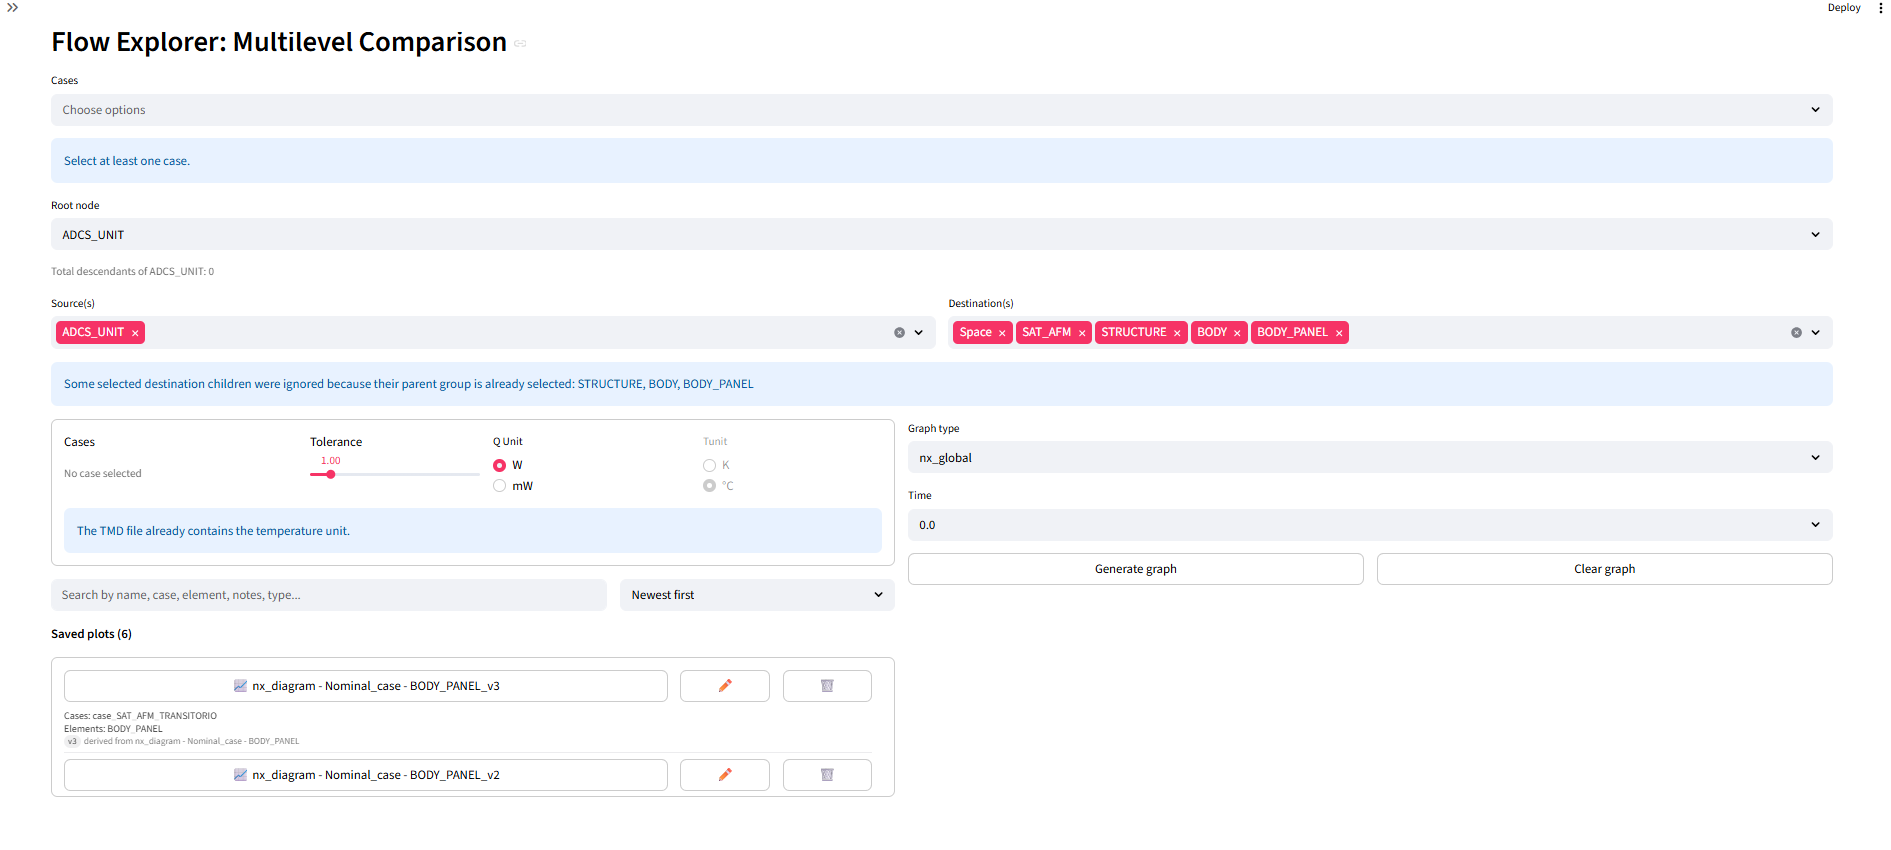
\includegraphics[
        width=\textwidth,
        height=0.76\textheight,
        keepaspectratio
    ]{Figures/Anexo_01/display01.png}
    \caption{Flow Explorer interface for hierarchical heat-flow inspection
    and multi-case representation.}
    \label{fig:appendix_flow_explorer}
\end{figure}

\clearpage

\begin{figure}[p]
    \centering
    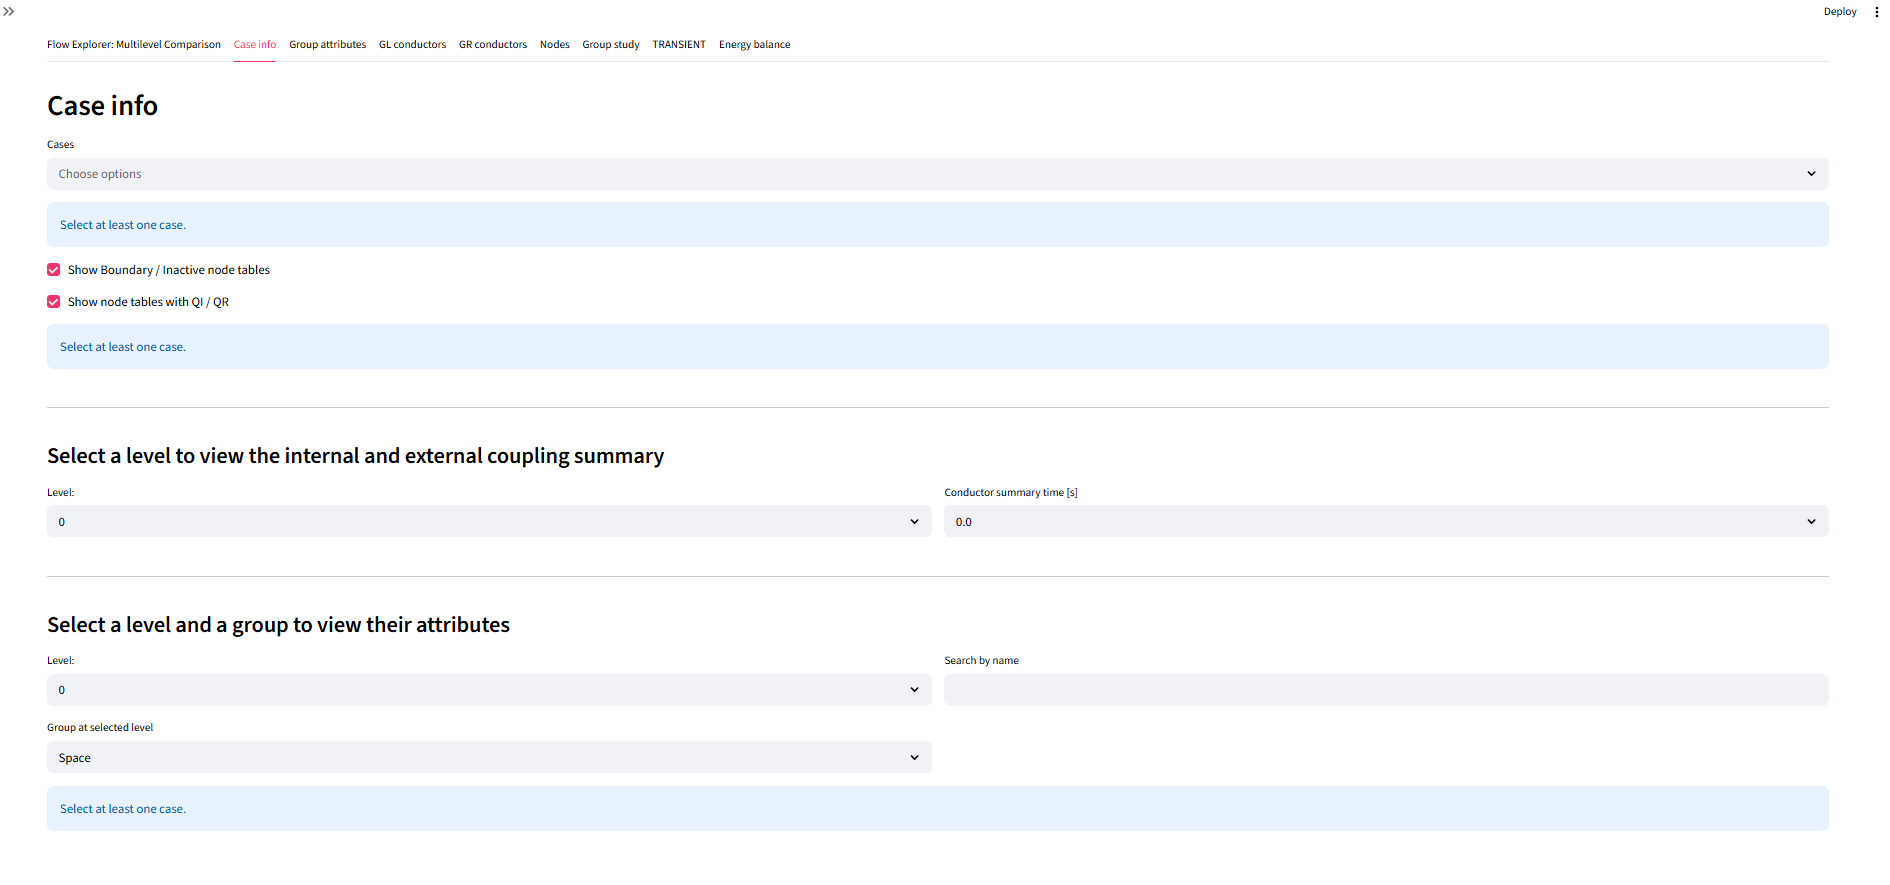
\includegraphics[
        width=\textwidth,
        height=0.76\textheight,
        keepaspectratio
    ]{Figures/Anexo_01/display02.png}
    \caption{Case-information interface showing the datasets, groups and
    couplings available in the loaded simulation.}
    \label{fig:appendix_case_information}
\end{figure}

\clearpage

\begin{figure}[p]
    \centering
    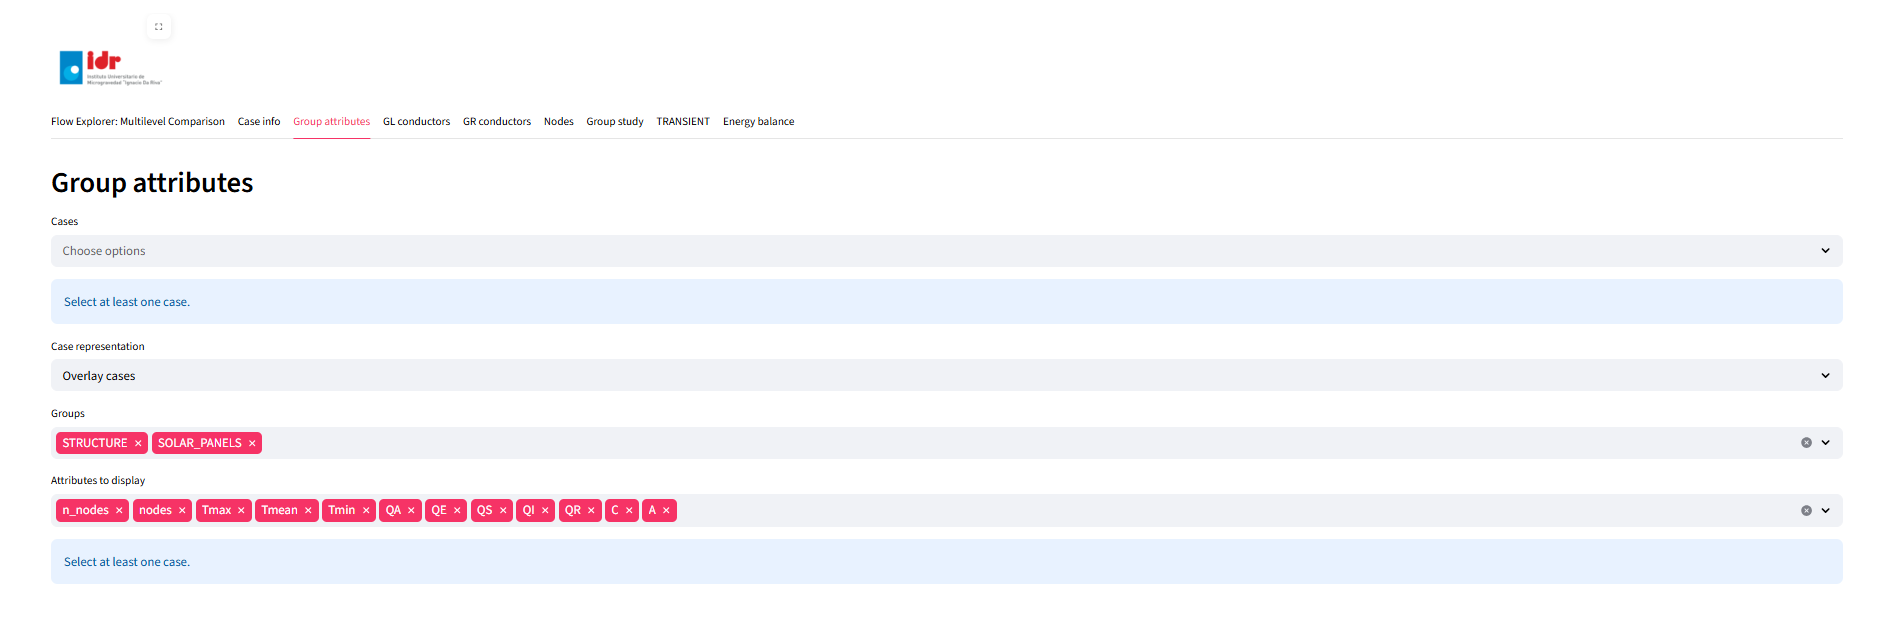
\includegraphics[
        width=\textwidth,
        height=0.76\textheight,
        keepaspectratio
    ]{Figures/Anexo_01/display03.png}
    \caption{Group-attribute interface for inspecting the selected model
    elements at a specified output instant.}
    \label{fig:appendix_group_attributes}
\end{figure}

\clearpage

\begin{figure}[p]
    \centering
    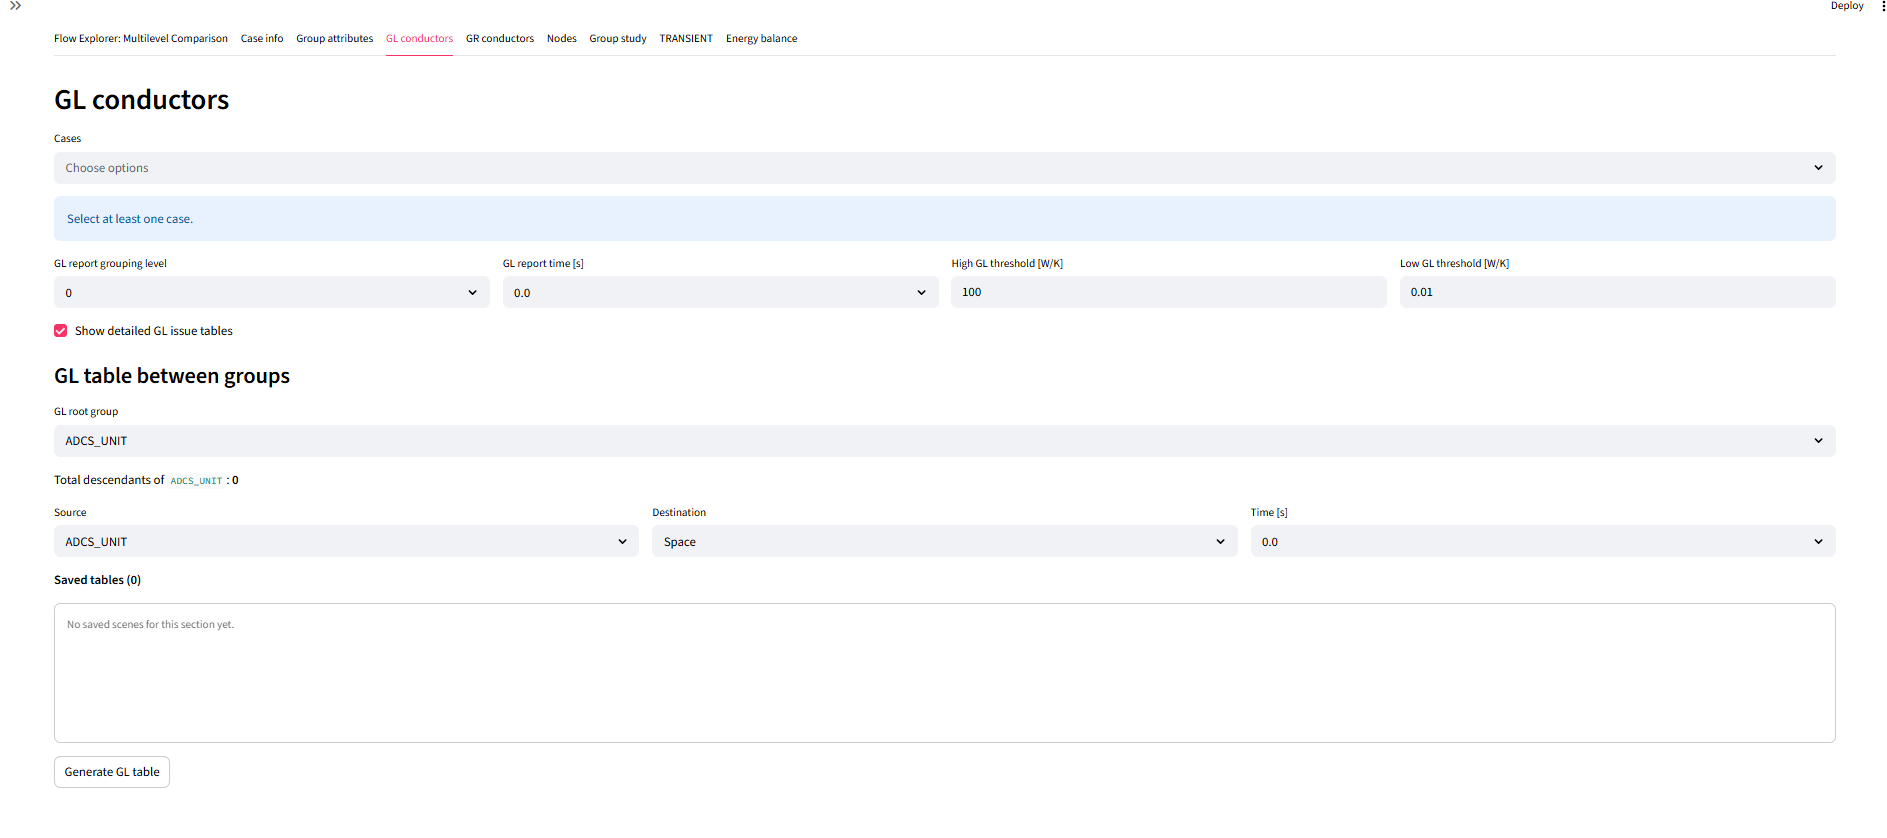
\includegraphics[
        width=\textwidth,
        height=0.76\textheight,
        keepaspectratio
    ]{Figures/Anexo_01/display04.png}
    \caption{Linear-conductor interface with case, group and output-time
    controls.}
    \label{fig:appendix_gl_conductors}
\end{figure}

\clearpage

\begin{figure}[p]
    \centering
    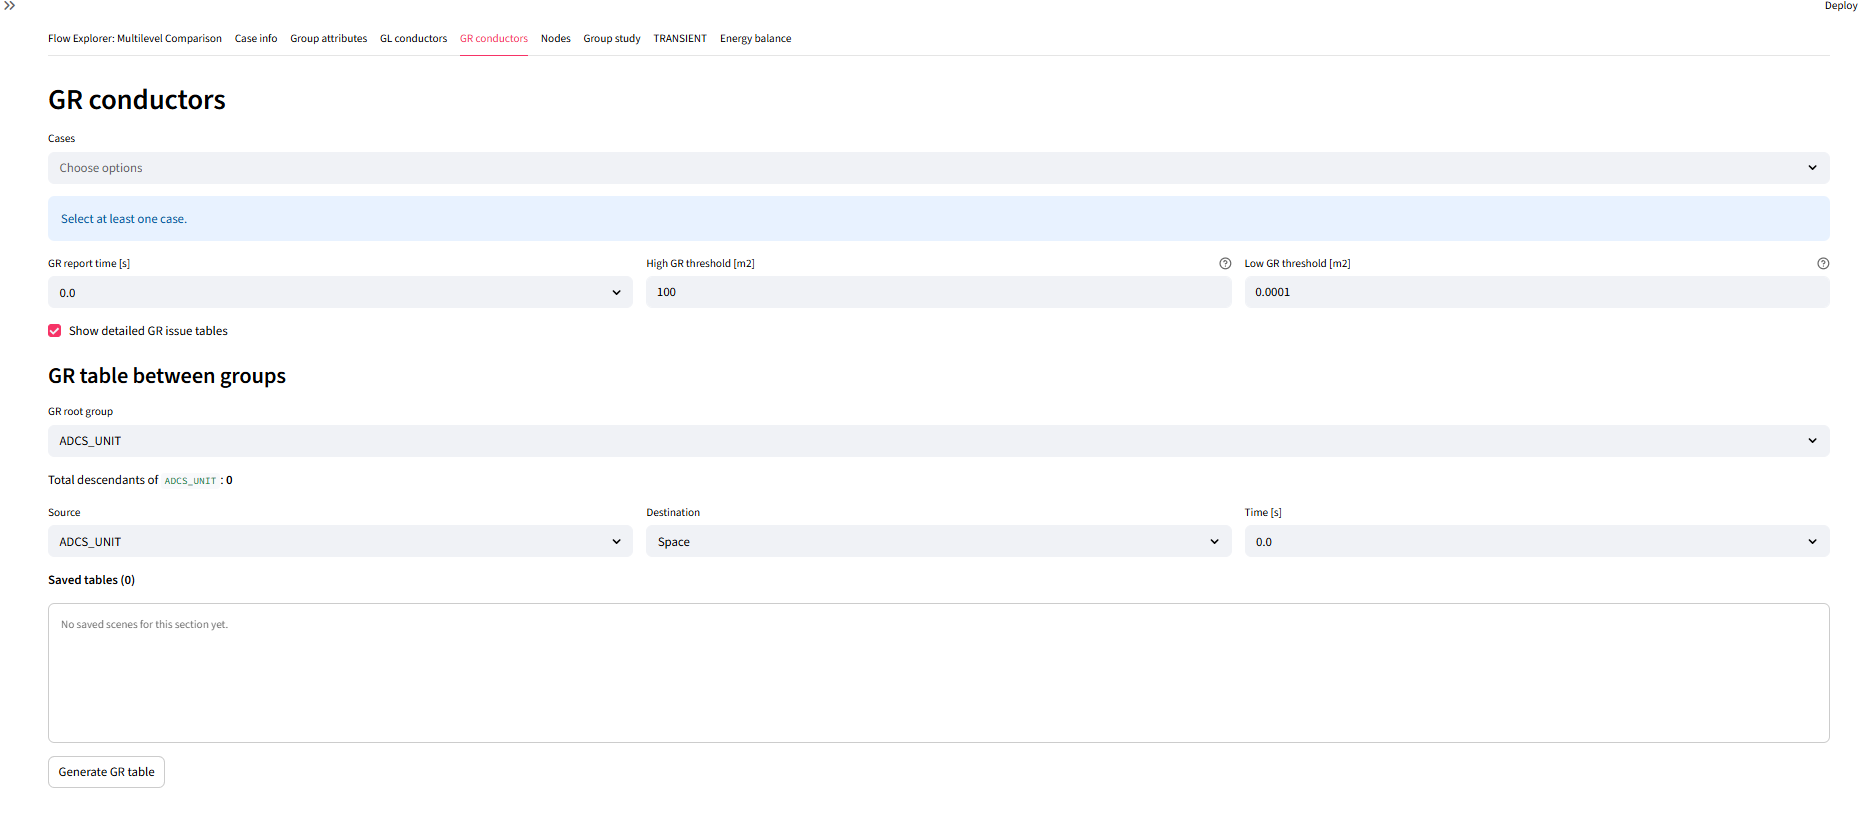
\includegraphics[
        width=\textwidth,
        height=0.76\textheight,
        keepaspectratio
    ]{Figures/Anexo_01/display05.png}
    \caption{Radiative-conductor interface with case, group and output-time
    controls.}
    \label{fig:appendix_gr_conductors}
\end{figure}

\clearpage

\begin{figure}[p]
    \centering
    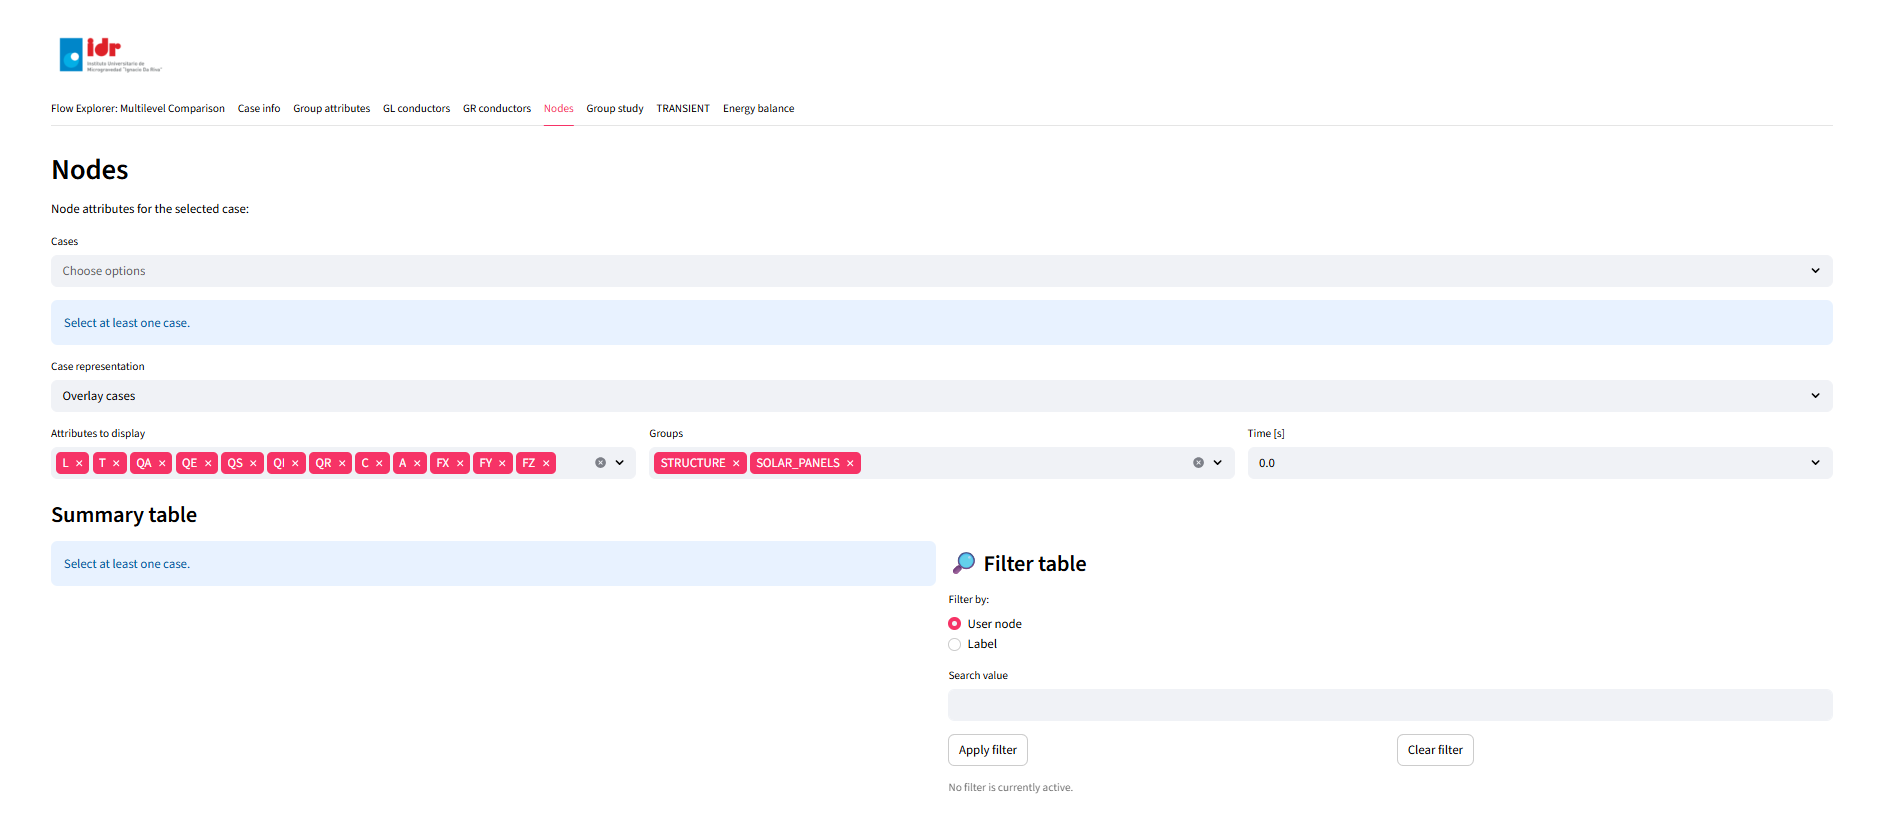
\includegraphics[
        width=\textwidth,
        height=0.76\textheight,
        keepaspectratio
    ]{Figures/Anexo_01/display06.png}
    \caption{Nodal-information interface for the selected hierarchy
    elements.}
    \label{fig:appendix_nodes}
\end{figure}

\clearpage

\begin{figure}[p]
    \centering
    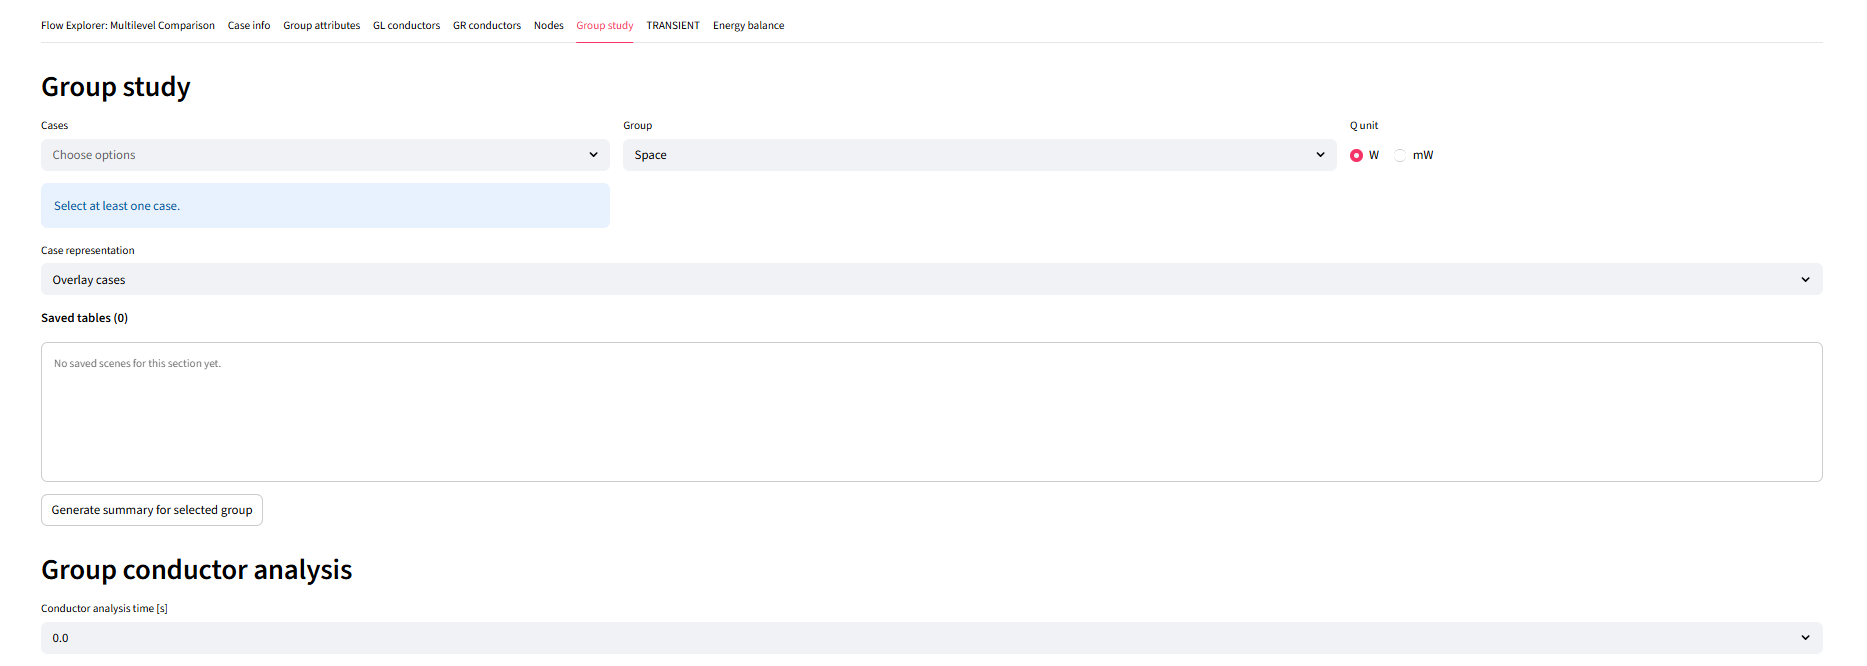
\includegraphics[
        width=\textwidth,
        height=0.76\textheight,
        keepaspectratio
    ]{Figures/Anexo_01/display07.png}
    \caption{Group-study interface for the inspection of selected components
    and their thermal connections.}
    \label{fig:appendix_group_study}
\end{figure}

\clearpage
\cleardoublepage

\hiddenappendixchapter
    {Secondary Implementation Improvements}
    {app:secondary_implementation_improvements}

\providecommand{\appBimage}[1]{%
    \IfFileExists{#1}{%
        \includegraphics[
            width=\linewidth,
            keepaspectratio
        ]{#1}%
    }{%
        \fbox{%
            \parbox[c][0.13\textheight][c]{0.92\linewidth}{%
                \centering
                \textbf{Capture pending}\\[0.6em]
                \texttt{\detokenize{#1}}
            }%
        }%
    }%
}

Several adaptations introduced during the development are secondary to the
transient and electrical methods described in the main chapters. They improve
selection consistency, temporal evaluation, conductor inspection, user
feedback, persistent storage and code organisation. The following sections
compare the relevant behaviour of the initial and final implementations and
document only functions present in the final application.

\section{Comparison of Initial and Final Behaviour}
\label{appsec:secondary_behaviour_comparison}

Table~\ref{tab:appendix_secondary_improvements} summarises the selected
adaptations. The comparison is based on the operation of both application
versions and on the final source-code organisation. It is not intended as a
complete change log, since the transient and electrical developments are
already described in Chapters~\ref{ch:multicase_tool},
\ref{ch:transient_analysis} and~\ref{ch:electrical_battery_analysis}.

% File: Tables/table_appendix_secondary_improvements.tex
\begingroup
\small
\renewcommand{\arraystretch}{1.12}
\setlength{\tabcolsep}{3pt}
\begin{longtable}{|>{\raggedright\arraybackslash}p{0.25\textwidth}|>{\raggedright\arraybackslash}p{0.35\textwidth}|>{\raggedright\arraybackslash}p{0.27\textwidth}|}
    \caption{Comparison of selected secondary implementation improvements.}
    \label{tab:appendix_secondary_improvements}\\
    \hline
    \textbf{Initial behaviour} & \textbf{Final behaviour} & \textbf{Main location} \\
    \hline
    \endfirsthead

    \multicolumn{3}{c}{\tablename\ \thetable\ -- continued}\\
    \hline
    \textbf{Initial behaviour} & \textbf{Final behaviour} & \textbf{Main location} \\
    \hline
    \endhead

    \hline
    \endfoot

    Group selectors were not consistently ordered according to the model
    structure. &
    Available groups follow the parent--child order defined by the Excel
    hierarchy, with fallback ordering for malformed or disconnected branches. &
    Common hierarchy-selection helpers and inherited group selectors. \\
    \hline
    Parent and descendant groups could be selected together and counted twice
    in aggregated results. &
    Descendants already included in a selected parent are removed and a visible
    message identifies the corrected selection. &
    Flow Explorer and compatible hierarchical selectors. \\
    \hline
    Several inherited modules evaluated only the active or first stored output
    state. &
    The selected value from the result-file time vector is applied to each
    compatible calculation and retained when the analysis is restored. &
    Flow Explorer, Group Attributes, GL/GR Conductors, Nodes and Group Study. \\
    \hline
    GL and GR inspection focused on individual source--target tables. &
    The final tabs also provide matrix-quality summaries, configurable high and
    low thresholds and detailed issue tables. &
    GL Conductors and GR Conductors. \\
    \hline
    Nodal filtering was applied while the filter text was being entered. &
    Separate \textit{Apply filter} and \textit{Clear filter} controls preserve
    an explicit active-filter state. &
    Nodes. \\
    \hline
    Interface candidates could be selected from hierarchy groups without
    confirming an explicit thermal connection. &
    GL and GR definitions are scanned to identify connected target groups and
    node pairs before the interface calculation. &
    Transient interface analysis. \\
    \hline
    Temperature changes over prescribed time intervals were not available as a
    complete analysis area. &
    Maximum and minimum temperature changes are calculated over selectable
    10-, 15-, 30- and 60-minute windows and summarised by group. &
    Transient temperature-variation analysis. \\
    \hline
    Validation and feedback differed between individual interface blocks. &
    Missing cases, empty selections and unavailable data produce visible
    messages before the calculation continues. &
    All final analysis modules. \\
    \hline
    Saving logic was distributed among individual output areas. &
    Saved analyses share a common database, file store, restoration recipe and
    editing workflow. &
    Scene-management and restoration modules. \\
    \hline
    Most interface areas were concentrated in the main application script. &
    The launcher, analysis tabs, shared helpers and persistence functions are
    separated into dedicated modules. &
    Application architecture. \\
    \hline
\end{longtable}
\endgroup


\section{Hierarchy Safeguards and Time-Dependent Inspection}
\label{appsec:hierarchy_time_safeguards}

Hierarchy-aware selection prevents the same physical branch from being
included more than once in an aggregated result. Figure~
\ref{fig:appendix_hierarchy_warning} shows the message produced when a parent
group and one or more of its descendants are selected simultaneously. The
descendants are removed because their nodes are already contained in the
parent selection.

\begin{figure}[!htbp]
    \centering
    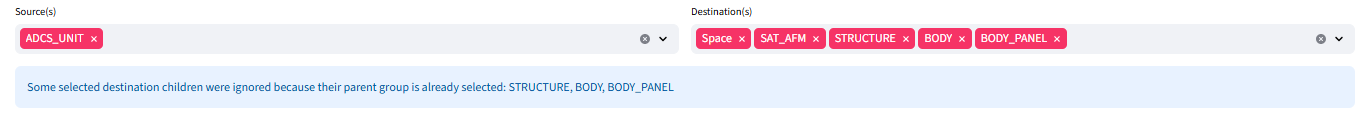
\includegraphics[
        width=0.94\textwidth,
        keepaspectratio
    ]{Figures/Anexo_02/hierarchy_selection_warning.png}
    \caption{Automatic removal of redundant descendant groups.}
    \label{fig:appendix_hierarchy_warning}
\end{figure}

The inherited modules use the output-time vector stored in each transient
result file. The selected instant is evaluated independently in each tab so
that its configuration can be saved and restored together with the remaining
controls. Table~\ref{tab:appendix_time_dependent_modules} identifies the
result evaluated at that instant.

% File: Tables/table_appendix_time_dependent_modules.tex
\begin{table}[H]
    \centering
    \caption{Use of the selected output time in the inherited modules.}
    \label{tab:appendix_time_dependent_modules}
    \small
    \renewcommand{\arraystretch}{1.13}
    \setlength{\tabcolsep}{3pt}
    \begin{tabularx}{\textwidth}{|>{\raggedright\arraybackslash}p{0.18\textwidth}|>{\raggedright\arraybackslash}X|>{\raggedright\arraybackslash}X|}
        \hline
        \textbf{Module} & \textbf{Time-dependent output} & \textbf{Stored setting} \\
        \hline
        Flow Explorer &
        Instantaneous source--target heat flows used by the selected graph. &
        Output time, groups, units, tolerance and graph type. \\
        \hline
        Group Attributes &
        Group temperatures, thermal loads and selected metadata. &
        Output time, cases, groups, attributes and representation mode. \\
        \hline
        GL Conductors &
        Linear-conductor values between the selected source and target. &
        Output time, groups and case selection. \\
        \hline
        GR Conductors &
        Radiative-conductor values between the selected source and target. &
        Output time, groups and case selection. \\
        \hline
        Nodes &
        Nodal temperatures, loads and selected node attributes. &
        Output time, cases, groups, attributes and active filter. \\
        \hline
        Group Study &
        Group summary and internal or external conductor values. &
        Output time, case, group, conductor type and units. \\
        \hline
    \end{tabularx}
\end{table}


Figure~\ref{fig:appendix_time_controls} provides two representative examples.
The Group Attributes selector is populated from the transient result vector,
whereas the GL tab uses the chosen time when generating the conductor table.
Equivalent controls are used by the remaining compatible modules.

\begin{figure}[H]
    \centering

    \begin{subfigure}[t]{0.48\textwidth}
        \centering
        \appBimage{Figures/Anexo_02/time_control_group_attributes.png}
        \caption{Group Attributes.}
        \label{fig:appendix_time_group_attributes}
    \end{subfigure}
    \hfill
    \begin{subfigure}[t]{0.48\textwidth}
        \centering
        \appBimage{Figures/Anexo_02/time_control_gl_conductors.png}
        \caption{GL Conductors.}
        \label{fig:appendix_time_gl_conductors}
    \end{subfigure}

    \caption{Representative output-time controls in inherited modules.}
    \label{fig:appendix_time_controls}
\end{figure}

\FloatBarrier

\section{Conductor Inspection and Interface Detection}
\label{appsec:conductor_interface_detection}

The GL and GR tabs include matrix-level diagnostics in addition to the
source--target tables described in Appendix~
\ref{app:inherited_interface_evolution}. The summaries report the number of
couplings and classify values according to configurable high and low
thresholds. Detailed issue tables can then isolate the affected pairs and be
saved independently.

\begin{figure}[!htbp]
    \centering

    \begin{subfigure}[t]{0.48\textwidth}
        \centering
        \appBimage{Figures/Anexo_02/gl_matrix_quality_summary.png}
        \caption{GL matrix summary.}
        \label{fig:appendix_gl_matrix_summary}
    \end{subfigure}
    \hfill
    \begin{subfigure}[t]{0.48\textwidth}
        \centering
        \appBimage{Figures/Anexo_02/gr_matrix_quality_summary.png}
        \caption{GR matrix summary.}
        \label{fig:appendix_gr_matrix_summary}
    \end{subfigure}

    \caption{Matrix-quality summaries available in the conductor tabs.}
    \label{fig:appendix_conductor_matrix_summaries}
\end{figure}

The transient interface analysis uses the same explicit connection data to
restrict the destination selector when the conductor filter is active. Only
node pairs connected through GL or GR definitions are evaluated. The
hierarchy remains available as a fallback when no explicit target is detected.

\begin{figure}[!htbp]
    \centering
    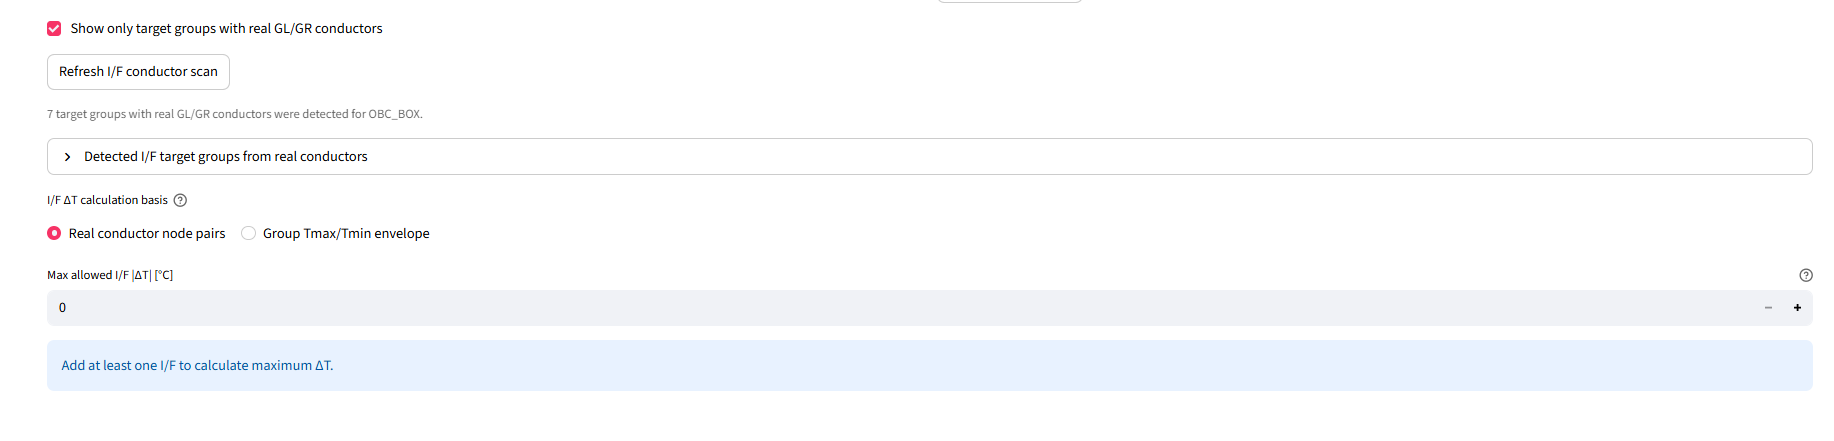
\includegraphics[
        width=0.94\textwidth,
        keepaspectratio
    ]{Figures/Anexo_02/interface_conductor_filter.png}
    \caption{Conductor-based filtering of candidate interface groups.}
    \label{fig:appendix_interface_conductor_filter}
\end{figure}

Table~\ref{tab:appendix_obc_detected_targets} provides a numerical example for
\texttt{OBC\_BOX}. The target groups and pair counts are obtained from the
same connection scan used to populate the interface selector. The table
documents the connection basis applied before the temperature differences are
calculated.

% File: Tables/table_appendix_obc_detected_targets.tex
% Usage: \AppendixOBCDetectedTargetsTable[0.94\textwidth]

\newcommand{\AppendixOBCDetectedTargetsTable}[1][0.94\textwidth]{%
\begin{table}[!htbp]
    \centering
    \caption{Target groups detected from the explicit GL and GR connections
    to \texttt{OBC\_BOX} in the nominal case.}
    \label{tab:appendix_obc_detected_targets}
    \renewcommand{\arraystretch}{1.16}
    \setlength{\tabcolsep}{4pt}
    \resizebox{#1}{!}{%
    \begin{tabular}{@{}lrrrrr@{}}
        \toprule
        \textbf{Target group} &
        \textbf{GL pairs} &
        \textbf{$\sum |GL|$ [W/K]} &
        \textbf{GR pairs} &
        \textbf{$\sum |GR|$ [m$^2$]} &
        \textbf{Total pairs} \\
        \midrule
        \texttt{BODY} & 4 & 22.68 & 559 & 0.355732 & 563 \\
        \texttt{RADIATOR} & 4 & 0.40 & 181 & 0.020584 & 185 \\
        \texttt{BODY\_PLATE\_MED} & 4 & 22.68 & 96 & 0.115546 & 100 \\
        \texttt{BODY\_PANEL} & 0 & 0.00 & 364 & 0.147134 & 364 \\
        \texttt{BODY\_PLATE\_SUP} & 0 & 0.00 & 91 & 0.092968 & 91 \\
        \texttt{Space} & 0 & 0.00 & 24 & 0.001042 & 24 \\
        \texttt{BODY\_PLATE\_INF} & 0 & 0.00 & 8 & 0.000083 & 8 \\
        \bottomrule
    \end{tabular}%
    }
\end{table}%
}

\AppendixOBCDetectedTargetsTable[0.94\textwidth]

\FloatBarrier

\section{Input Validation and User Feedback}
\label{appsec:validation_feedback}

The final interface checks the information required by each calculation before
processing begins. Missing cases, empty group selections, unsupported
combinations and unavailable conductor data produce visible messages instead
of incomplete outputs or uncaught errors. Figure~
\ref{fig:appendix_validation_no_case} shows the response when no case has been
selected. Equivalent checks are applied locally by the remaining modules.

\begin{figure}[!htbp]
    \centering
    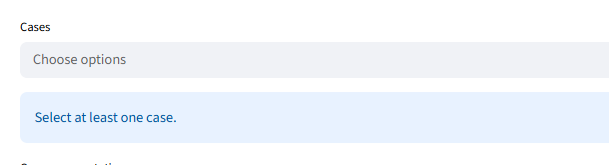
\includegraphics[
        width=0.72\textwidth,
        keepaspectratio
    ]{Figures/Anexo_02/validation_no_case.png}
    \caption{Validation message displayed when no case is selected.}
    \label{fig:appendix_validation_no_case}
\end{figure}

\section{Persistent Analysis Storage}
\label{appsec:persistent_analysis_storage}

The saving workflow described in Section~\ref{sec:analysis_saving_export}
uses an SQLite database together with a structured file store. The database
relates each saved analysis to its model, cases, source tab, model element and
stored recipe. The file directory contains the generated representations and
a JSON description of the settings required for restoration.

A saved entry follows the general structure below. The exact intermediate
folders depend on whether the output belongs to one case, several cases or a
case-difference comparison.

\begin{lstlisting}[basicstyle=\ttfamily\small, frame=single]
scene_store/
+-- <model>/
    +-- <scope_and_cases>/
        +-- <element_type>_<element>/
            +-- scene_<timestamp>_<tab>_<name>/
                +-- scene.json
                +-- figure.plotly.json
                +-- figure.html
                +-- table.csv
                +-- table.xlsx
                +-- figure.png
                +-- figure.svg
\end{lstlisting}

Only the files associated with the generated output are created. Plotly
figures produce JSON and HTML files, data tables produce CSV and spreadsheet
files, and Matplotlib figures produce PNG and SVG images. The metadata file is
always written.

% File: Tables/table_appendix_saved_analysis_artifacts.tex
\begin{table}[!htbp]
    \centering
    \caption{Files and records associated with a saved analysis.}
    \label{tab:appendix_saved_analysis_artifacts}
    \small
    \renewcommand{\arraystretch}{1.14}
    \setlength{\tabcolsep}{4pt}
    \begin{tabularx}{\textwidth}{|>{\raggedright\arraybackslash}p{0.26\textwidth}|>{\raggedright\arraybackslash}X|}
        \hline
        \textbf{Stored item} & \textbf{Purpose} \\
        \hline
        SQLite model, case and analysis records &
        Relate the saved output to its source files, visible case names,
        element, tab and creation metadata. \\
        \hline
        Recipe JSON in the database &
        Stores widget values required to restore the analysis configuration. \\
        \hline
        \texttt{scene.json} &
        Provides a readable file copy of the saved metadata and recipe. \\
        \hline
        \texttt{figure.plotly.json} and \texttt{figure.html} &
        Preserve an interactive Plotly figure and provide an independent
        browser representation. \\
        \hline
        \texttt{table.csv} and \texttt{table.xlsx} &
        Preserve a generated numerical table in two conventional formats. \\
        \hline
        \texttt{figure.png} and \texttt{figure.svg} &
        Preserve a Matplotlib figure for reports and scalable editing. \\
        \hline
    \end{tabularx}
\end{table}


Consistency checks remove database entries whose folders no longer exist and
scene folders that are no longer referenced by the database. An auxiliary
cleanup script creates backups before removing saved analyses unrelated to a
defined set of retained model files. These functions reduce stale references
without changing the original \texttt{.TMD} or hierarchy files.

\section{Source-Code Reorganisation}
\label{appsec:source_code_reorganisation}

The initial interface concentrates the inherited tabs in a single application
script. The final organisation separates each analysis area from the launcher
and isolates saving and restoration functions in dedicated modules. This
structure allows one tab to be modified without rewriting the complete
interface and supports the addition of the transient and electrical modules.

% File: Tables/table_appendix_code_reorganisation.tex
\begingroup
\footnotesize
\renewcommand{\arraystretch}{1.06}
\setlength{\tabcolsep}{3pt}
\begin{longtable}{|>{\raggedright\arraybackslash}p{0.32\textwidth}|>{\raggedright\arraybackslash}p{0.58\textwidth}|}
    \caption{Correspondence between the initial interface blocks and the final modules.}
    \label{tab:appendix_code_reorganisation}\\
    \hline
    \textbf{Initial block} & \textbf{Final module} \\
    \hline
    \endfirsthead

    \multicolumn{2}{c}{\tablename\ \thetable\ -- continued}\\
    \hline
    \textbf{Initial block} & \textbf{Final module} \\
    \hline
    \endhead

    \hline
    \endfoot

    Flow Explorer block in \texttt{app\_interactiva.py} &
    \texttt{tabs/tab\_flow\_explorer.py} \\
    \hline
    Model-information block &
    \texttt{tabs/tab\_case\_info.py} \\
    \hline
    Group-attribute block &
    \texttt{tabs/tab\_group\_attributes.py} \\
    \hline
    GL and GR blocks &
    \texttt{tabs/tab\_gl\_conductors.py} and
    \texttt{tabs/tab\_gr\_conductors.py} \\
    \hline
    Nodes and group-study blocks &
    \texttt{tabs/tab\_nodes.py} and
    \texttt{tabs/tab\_group\_study.py} \\
    \hline
    Initial transient prototype &
    \texttt{tabs/tab\_transient.py} \\
    \hline
    Solar and battery calculations &
    \texttt{tabs/tab\_sp.py} \\
    \hline
    Saving and restoration functions &
    \texttt{app\_thermalviewer/scene\_manager.py},
    \texttt{scene\_ui.py}, \texttt{restored\_scenes.py} and
    \texttt{scene\_editor.py} \\
    \hline
    Common widget, hierarchy and export routines &
    \texttt{app\_thermalviewer/app\_helpers.py} and
    \texttt{viewer\_utils.py} \\
    \hline
\end{longtable}
\endgroup


The reorganisation changes only the software structure; all modules continue
to share the same imported case and hierarchy objects.

\FloatBarrier

\cleardoublepage

\end{document}